\documentclass[9pt]{report}

\usepackage[a4paper,left=1.3cm,right=1.5cm,top=3cm,bottom=2.5cm,bindingoffset=5mm]{geometry}
\usepackage[ngerman,english]{babel}
\usepackage[utf8]{inputenc}
\usepackage[T1]{fontenc}
\usepackage{lmodern}
\usepackage{amsmath}
\usepackage{amssymb}
\usepackage{bbm}
\usepackage{tabularx}
\usepackage{graphicx}
\usepackage{siunitx}
\usepackage{array}
\usepackage{ragged2e}
\usepackage{hyperref}
\usepackage{float}
\usepackage{listings}
\usepackage{color}
\usepackage{subcaption}
\usepackage[dvipsnames]{xcolor}
\usepackage[theorems]{tcolorbox}
\usepackage{fancyhdr}
\usepackage{autobreak}
%\usepackage{picins}


\pagestyle{fancy}

\fancyhf{}

\lhead{\rightmark}
\chead{}
\rhead{\thepage}

\lfoot{}
\cfoot{}
\rfoot{}




\lstset{language=Python, 
        columns=flexible, 
        numbers=left, 
        xleftmargin=1.3em, 
        basicstyle=\footnotesize\ttfamily, 
        keywordstyle=\color{blue}, 
        morekeywords={as}, 
        stringstyle=\color{green}}


%\tcbset{defstyle/.style={
%		fonttitle=\sffamily\bfseries,
%		arc=0mm,
%		colback=blue!10,
%		colframe=green,
%		separator sign none}}




\title{\Huge\textbf{Quantum Chemistry}}
\date{}
\author{}





\begin{document}

\maketitle


\tableofcontents

\newpage
\chapter{Quantum Chemistry}
$"$Dem Anwenden muss das Erkennen vorausgehen.$"$ (Max Planck)\\
$"$Jeder Versuch mathematische Methoden zur Untersuchung chemischer Fragestellungen zu benutzen muß als völlig irrational und gegen den Geist der Chemie gerichtet angesehen werden. Falls die Mathematik jemals einen prominenten Platz in der Chemie einnehmen sollte - eine Verirrung, die glücklicherweise fast unmöglich ist - würde diese zum schnellen und irreversiblen Niedergang dieser Wissenschaft führen.$"$ (Isidor Marie Auguste Francois Xavier Comte, 1836)\\
$"$Die grundlegenden physikalischen Gesetze zur mathematischen Behandlung großer Teile der Physik und der gesamten Chemie sind vollständig bekannt. Die Schwierigkeit besteht nur darin, dass die exakte Anwendung dieser Gesetze zu Gleichungen führt, die viel zu kompliziert sind, als dass man sie lösen könnte.$"$ (Paul Dirac, 1929)\\
$"$Eine neue Theorie ist etwas woran keiner glaubt, außer demjenigen, der sie gemacht hat. Ein neues Experiment ist etwas, woran alle glauben, außer demjenigen, der es gemacht hat.$"$ (Albert Einstein)\\
$"$Ein empirisch-wissenschaftliches System muss an der Erfahrung scheitern können.$"$ (Karl Raimund Popper, 1973)\\
$"$Experimente sind die einzige Quelle des Wissens, die uns zur Verfügung steht. Der Rest ist Poesie und Imagination.$"$ (Max Planck)\\
$"$Computers don't solve problems. People do.$"$ (Ernest R. Davidson)\\
$"$It is nice to know that the computer understands the problem. But I would like to understand it too.$"$ (Eugene Paul Wigner)\\
$"$Erstens kann man mit Recht sagen, dass wir nicht mit einzelnen Partikeln experimentieren, genauso wenig wie wir Ichthyosaurus im Zoo aufziehen können. Dies ist die offensichtliche Tatsache, dass wir niemals mit nur einem Elektron, Atom oder (kleinen) Molekül experimentieren. In Gedankenexperimenten nehmen wir manchmal an, dass wir es tun. Dies hat immer lächerliche Konsequenzen.$"$ (Erwin Schrödinger)\\
$"$...wir werden später noch lächerlicher sein und Bits betrachten, die auf ein Atom geschrieben werden, anstatt auf die gegenwärtig 10$^{11}$ Atome. Ein solcher Unsinn ist für Professoren wie mich sehr unterhaltsam. Ich hoffe, Sie werden es auch interessant und unterhaltsam finden.$"$ (Richard Feynman, 1986)




\newpage
\section{Mathematischer Formalismus}

\subsection{Vektorräume, Skalarprodukte und Normen}
\subsection{Hilberträume}
In quantum mechanics, the state of a physical system is described by the specification of a complex state vector $|\Psi\rangle$. The state space of a physical system is a Hilbert space $\mathcal{H}$. The most important Hilbert space considered in quantum mechanics is the infinite-dimensional space of square-integrable functions $L^2(\mathbb{R}^n)$, which is defined as
\begin{equation}
L^2(\mathbb{R}^n)\equiv\bigg\{\psi:\mathbb{R}^{n}\to\mathbb{C}\,;\int|\psi(x)|^2\mathrm{d}^{n}x\;<\infty\bigg\}
\end{equation}
In this space an inner product can be defined by
\begin{equation}
\langle\psi,\phi\rangle=\int\psi^{*}(x)\phi(x)\,\mathrm{d}^{n}x
\end{equation}
which induces the $L^2$-norm
\begin{equation}
\Vert\psi\Vert_{L^2}=\bigg(\int|\psi(x)|^2\mathrm{d}^{n}x\bigg)^{1/2}
\end{equation}


\subsection{Tensorprodukte}


\subsection{Orthonormalbasen}
Let $V$ be an inner product space. Then a set $(e_i)_{i\in I}$ of vectors $e_1,e_n,...\in V$ is called orthonormal if the following conditions are fulfilled for all $e_i\in V$:
\begin{itemize}
\item $\langle e_i,e_j\rangle =0\quad\forall\;e_i,e_j\in V$\quad (pairwise orthogonality)
\item $\Vert e_i\Vert =\sqrt{\langle e_i,e_i\rangle}=1\quad\forall\;e_i\in V$\quad (normalization)
\end{itemize}
These conditions for a set of orthonormal vectors can be compactly represented by the Kronecker delta: 
\begin{equation}
\langle e_i,e_j\rangle =\delta_{ij}=\left\{\begin{array}{cc} 1 & \textrm{if}\;\; i=j\\
0 & \textrm{if}\;\; i\neq j\\ \end{array}\right.
\end{equation}
When a set of orthonormal vectors simultaneously fulfills the conditions for a basis, it is called a complete orthonormal system or orthonormal basis (ONB). A big advantage of orthonormal bases compared to conventional bases lies in the simplifying of calculations.


\subsubsection{Endlichdimensionale Räume}
Sei $V$ ein endlichdimensionaler Prähilbertraum und sei $\langle U\rangle=\mathrm{span}(e_1,...,e_n)$, wobei die $e_j$ ein VONS bilden. Dann lassen sich die Komponenten eines Vektors $v\in \langle U\rangle$ bezüglich dieser Basis besonders leicht über das Skalarprodukt berechnen:
\begin{equation}
v=\sum_{j=1}^{n}\langle v,e_j\rangle e_j
\end{equation}
Diese Aussage lässt sich leicht beweisen: Da $U$ ein Erzeugendensystem bildet, hat jeder Vektor $v$ eine Darstellung $v=\sum_{j=1}^{n}\lambda_{j}e_{j}$ mit eindeutig bestimmten $\lambda_j\in\mathbb{K}$. Genau diese Darstellung ergibt sich durch Einsetzen der Linearkombination in das Skalarprodukt:
\begin{equation}
\langle v,e_i\rangle =\Bigg\langle\sum_{j=1}^{n}\lambda_{j}e_{j},e_{i}\Bigg\rangle =\sum_{j=1}^{n}\lambda_{j}\langle e_j,e_i\rangle =\sum_{j=1}^{n}\lambda_{j}\delta_{ji}=\lambda_j\notag
\end{equation}

Das Skalarprodukt zwischen zwei Vektoren nimmt in einem VONS eine besonders einfache Komponentendarstellung an. Seien $V$ ein endlichdimensionaler unitärer Vektorraum, $u,v\in V$ und $\alpha,\beta\in\mathbb{C}$, dann gilt für das Skalarprodukt:
\begin{equation}
\langle u,v\rangle =\Bigg\langle\sum_{j=1}^{n}\alpha_j e_j,\sum_{k=1}^{n}\beta_k e_k\Bigg\rangle =\sum_{j=1}^{n}\alpha_{j}^{*}\sum_{k=1}^{n}\beta_{k}\langle e_j,e_k\rangle =\sum_{j=1}^{n}\sum_{k=1}^{n}\alpha_{j}^{*}\beta_{k}\delta_{jk}=\sum_{j=1}^{n}\alpha_{j}^{*}\beta_{j}\notag
\end{equation}
Mit $v\in V$ und $\lambda\in\mathbb{C}$ ergibt sich in einem VONS für die durch das Skalarprodukt induzierte Norm die Darstellung
\begin{equation}
\Vert v\Vert =\sqrt{\langle v,v\rangle}=\sqrt{\Bigg\langle\sum_{j=1}^{n}\lambda_j e_j,\sum_{k=1}^{n}\lambda_{k}e_k\Bigg\rangle}=\sqrt{\sum_{j=1}^{n}\sum_{k=1}^{n}\lambda_{j}^{*}\lambda_{k}\delta_{jk}}=\sqrt{\sum_{j=1}^{n}\vert\lambda_j\vert^{2}}\notag
\end{equation}

Mit Hilfe des \textsc{Gram-Schmidt}schen Orthonormalisierungsverfahrens kann aus jeder endlichen oder unendlichen Familie linear unabhängiger Vektoren $(v_1,...,v_n)$ aus einem Prähilbertraum ein Orthonormalsystem erzeugt werden, das denselben Unterraum erzeugt. Verwendet man ein System von Basisvektoren, so berechnet der Algorithmus ein VONS.
Die einzelnen Vektoren $e_1,...,e_n$ des Orthonormalsystems erhält man nach folgender Vorschrift:
\begin{align}
e_1 & :=\frac{v_1}{\Vert v_1\Vert}\notag\\
e_i & :=\frac{e_1'}{\Vert e_i'\Vert}\quad\mathrm{mit}\quad e_i'=v_i -\sum_{j=1}^{i-1}\langle v_i,e_j\rangle e_j\qquad\forall\;i\geq 2\notag
\end{align}

Als Beispiel für die Komponentendarstellung von Skalarprodukt und Norm in einem VONS wird  zunächst der Koordinatenraum $\mathbb{C}^n$ mit der Standard-ONB
\begin{equation}
\{e_1,e_2,...,e_n\}=\{(1,0,...,0),(0,1,...,0),...,(0,...,0,1)\}
\end{equation}
betrachtet. Nach der obigen Vorschrift für die Komponentendarstellung von Skalarprodukten in VONS lässt sich dann das Standardskalarprodukt zweier komplexer Vektoren $x,y\in\mathbb{C}^n$ auf folgende Weise definieren:
\begin{equation}
\langle x,y\rangle =\sum_{i=1}^{n}x_{i}^{*}y_i =x^{\dagger}y
\end{equation}
Die durch das Standardskalarprodukt induzierte Norm wird euklidische Norm genannt. Ihre Darstellung in einem VONS ergibt sich ebenfalls nach der obigen Vorschrift:
\begin{equation}
\Vert x\Vert_{2}=\Bigg(\sum_{i=1}^{n}\vert x_i\vert^{2}\Bigg)^{1/2}
\end{equation}

Auf einem Matrizenraum, z.B. dem $\mathbb{C}^{m\times n}$, lässt sich ebenfalls ein Skalarprodukt definieren. Damit wird auch der Matrizenraum zu einem Prähilbertraum. Die Standard-ONB eines Matrizenraumes bilden die Standard-Einheitsmatrizen. Eine Standard-Einheitsmatrix $E_{kl}=(a_{ij})\in\mathbb{C}^{m\times n}$ ist die Matrix mit den Einträgen
\begin{equation}
a_{ij}=\left\{\begin{array}{ccc} 1 & \textrm{für} & \; k=i\;\mathrm{und}\;l=j\\
0 & \textrm{für} & \;\mathrm{sonst}\\ \end{array}\right.
\end{equation}
für $i=1,...,m$ und $j=1,...,n$. Bei der Standard-Einheitsmatrix $E_{kl}$ ist demnach der Eintrag an der Stelle $(k,l)$ gleich eins und alle anderen Einträge gleich null. Jede Matrix $A\in \mathbb{C}^{m\times n}$ lässt sich somit als Linearkombination von Standard-Einheitsmatrizen durch
\begin{equation}
A=\sum_{i=1}^{m}\sum_{j=1}^{n}a_{ij}E_{ij}
\end{equation}
mit $a_{ij}\in\mathbb{C}$ darstellen. Für das Skalarprodukt zwischen zwei Matrizen ergibt sich damit:
\begin{align}
\langle A,B\rangle &=\Bigg\langle\sum_{i=1}^{m}\sum_{j=1}^{n}\alpha_{ij}E_{ij},\sum_{k=1}^{m}\sum_{l=1}^{n}\beta_{kl}E_{kl}\Bigg\rangle =\sum_{i=1}^{m}\sum_{j=1}^{n}\alpha_{ij}^{*}\sum_{k=1}^{m}\sum_{l=1}^{n}\beta_{kl}\langle E_{ij},E_{kl}\rangle\\
&=\sum_{i=1}^{m}\sum_{j=1}^{n}\sum_{k=1}^{m}\sum_{l=1}^{n}\alpha_{ij}^{*}\beta_{kl} =\sum_{i=1}^{m}\sum_{j=1}^{n}\alpha_{ij}^{*}\beta_{ij}=\mathrm{spur}(A^{\dagger}B)
\end{align}
Dieses Skalarprodukt wird als Frobenius-Skalarprodukt bezeichnet. Die durch das Frobenius-Skalarprodukt induzierte Matrixnorm wird als Frobeniusnorm bezeichnet:
\begin{equation}
\Vert A\Vert_{F}=\Bigg(\sum_{i=1}^{m}\sum_{j=1}^{n}\vert \alpha_{ij}\vert^{2}\Bigg)^{1/2}
\end{equation}










\subsubsection{Unendlichdimensionale Räume}
Im folgenden sei $V$ ein unendlichdimensionaler Prähilbertraum über $\mathbb{K}$ und $(e_i)_{i\in I}$ ein Orthonormalsystem. Es gilt der Satz, dass eine Reihenentwicklung
\begin{equation}
v=\sum_{j=1}^{\infty}\lambda_{j}e_{j}
\end{equation}
nur existieren kann, wenn
\begin{equation}
\lambda_{j}=\langle v, e_j\rangle\quad\forall\;j
\end{equation}
Dies ergibt sich aus
\begin{equation}
\langle v,e_i\rangle =\bigg\langle\sum_{j=1}^{\infty}\lambda_{j}e_{j},e_{i}\bigg\rangle =\sum_{j=1}^{\infty}\lambda_{j}\langle e_j,e_i\rangle =\sum_{j=1}^{\infty}\lambda_{j}\delta_{ji}=\lambda_j
\end{equation}
Wenn die Koeffizienten der Reihe so bestimmt werden, wird der Vektor $v$ auf bestmögliche Art approximiert, unabhängig davon, ob die Reihe den Vektor $v$ exakt wiedergibt oder ob die Reihe überhaupt gegen ein Element des Prähilbertraumes konvergiert. Daher gilt im Allgemeinen folgende Beziehung für die Bestapproximation eines Vektors im quadratischen Mittel:
\begin{equation}
\lim_{n\to\infty}\bigg\Vert v-\sum_{j=1}^{n}\langle v,e_j\rangle e_j\bigg\Vert^{2}\geq 0
\end{equation}
Eine aussagekräftigere Form dieser Beziehung erhält man, wenn folgende Umformungen durchgeführt werden:
\begin{align}
0&\leq\bigg\Vert v-\sum_{j=1}^{n}\langle v,e_j\rangle e_j\bigg\Vert^{2}\\
&=\bigg\langle v-\sum_{j=1}^{n}\langle v,e_j\rangle e_j,v-\sum_{i=1}^{n}\langle v,e_{i}\rangle e_i\bigg\rangle\\
&=\langle v,v\rangle-\bigg\langle v,\sum_{j=1}^{n}\langle v,e_j\rangle e_j\bigg\rangle-\bigg\langle\sum_{j=1}^{n}\langle v,e_j\rangle e_j,v\bigg\rangle+\bigg\langle\sum_{j=1}^{n}\langle v,e_j\rangle e_j,\sum_{i=1}^{n}\langle v,e_i\rangle e_i\bigg\rangle\\
&=\langle v,v\rangle-\sum_{j=1}^{n}\langle v,e_j\rangle\langle v,e_j\rangle-\sum_{j=1}^{n}\langle v,e_j\rangle\langle v,e_j\rangle+\sum_{j=1}^{n}\sum_{i=1}^{n}\langle v,e_j\rangle^{*}\langle v,e_i\rangle\delta_{ji}\\
&=\langle v,v\rangle-2\sum_{j=1}^{n}|\langle v,e_j\rangle|^{2}+\sum_{j=1}^{n}|\langle v,e_j\rangle|^{2}\\
&=\Vert v\Vert^2-\sum_{j=1}^{n}|\langle v,e_j\rangle|^{2}
\end{align}
Damit erhält man für $n\to\infty$ direkt die sogenannte Besselsche Ungleichung:
\begin{equation}
\sum_{j=1}^{\infty}|\langle v,e_j\rangle|^{2}\geq\Vert v\Vert^2
\end{equation}




\subsection{Selbstadjungierte Operatoren}




\subsection{Darstellungstheorie}
Wie oben beschrieben, werden in der Quantenmechanik alle Sätze von Eigenfunktionen von hermiteschen Operatoren als gleichberechtigt betrachtet, zum Beispiel
\begin{alignat*}{2}
\hat{H}|n\rangle&=E|n\rangle\qquad&(\mathrm{Hamiltonoperator})\\
\hat{x}|x\rangle&=x|x\rangle\qquad&(\mathrm{Ortsoperator})\\
\hat{p}|p\rangle&=p|p\rangle\qquad&(\mathrm{Impulsoperator})
\end{alignat*}
Wie im obigen Abschnitt $"$Selbstadjungierte und hermitesche Operatoren$"$ beschrieben wurde, bilden die Eigenfunktionen des Hamiltonoperators $\{|n\rangle,n=1,2,...\}$ eine Orthonormalbasis im Hilbertraum $L^2(\mathbb{R}^{n})$. Daher kann ein beliebiger Zustand $|\psi\rangle$ nach dieser ONB als verallgemeinerte Fourierreihe entwickelt werden:
\begin{equation}
|\psi\rangle=\sum_{n=1}^{\infty}a_{n}|n\rangle=\sum_{n=1}^{\infty}|n\rangle\langle n|\psi\rangle
\end{equation}
Der Ausdruck für die Entwicklungskoeffizienten $a_{n}$ ergibt sich durch Multiplikation mit den adjungierten Basisvektoren $\langle n'|$:
\begin{equation}
\langle n'|\psi\rangle=\sum_{n=1}^{\infty}a_{n}\langle n'|n\rangle=\sum_{n=1}^{\infty}a_{n}\delta_{n'n}=a_{n}
\end{equation}
Der Ausdruck
\begin{equation}
\mathbbm{1}=\sum_{n=1}^{\infty}|n\rangle\langle n|
\end{equation}
wird als 1-Operator bezeichnet. Ein beliebiger quantenmechanischer Zustand $|\psi\rangle$ kann auch nach den Eigenfunktionen des Orts- oder Impulsoperators entwickelt werden. Im Gegensatz zur Entwicklung nach Eigenfunktionen des Hamiltonoperators handelt es sich hierbei aber nicht um eine diskrete, sondern um eine kontinuierliche Basisentwicklung, da Orts- und Impulsoperator kein diskretes Spektrum besitzen. Da es aber in den zugrundeliegenden separablen Hilberträumen kein Kontinuum von paarweise orthogonalen Vektoren geben kann, handelt es sich nicht um eine Entwicklung nach Basisvektoren des Hilbertraums. Denn die Orts- und Impulseigenfunktionen sind keine Elemente des Raums $L^2(\mathbb{R}^{n})$. Trotzdem lässt man diese kontinuierlichen Basisentwicklungen, die auf verallgemeinerte Fouriertransformationen führen, zu, da die Fouriertransformation nichts an der Quadratintegrabilität des physikalisch relevanten Zustandsvektors $|\psi\rangle$ ändert. Im Gegensatz zur diskreten Basis wird die unendliche Summe durch ein Integral ersetzt, was im Falle der Ortseigenfunktionen auf folgende Entwicklung führt:
\begin{equation}
|\psi\rangle=\int\mathrm{d}^{n}x\,\psi(x)|x\rangle=\int\mathrm{d}^{n}x\,|x\rangle\langle x|\psi\rangle
\end{equation}
Wie für den diskreten Fall ergibt sich auch hier der Ausdruck für die $"$Entwicklungskoeffizienten$"$ $\psi(x)$ durch Multiplikation mit dem adjungierten Basisvektor $\langle x'|$:
\begin{equation}
\langle x'|\psi\rangle=\int\mathrm{d}^{n}x\,\psi(x)\langle x'|x\rangle=\int\mathrm{d}^{n}x\,\psi(x)\delta(x'-x)=\psi(x)
\end{equation}
Der 1-Operator hat die Form
\begin{equation}
\mathbbm{1}=\int\mathrm{d}^{n}x\,|x\rangle\langle x|
\end{equation}
In der untenstehenden Tabelle sind die sich aus einer bestimmten Basisdarstellung ergebenden mathematischen Ausdrücke zusammenfassend dargestellt.

\begin{table}[h]
\textbf{\caption{Vergleich der mathematischen Struktur einer diskreten und einer kontinuierlichen Basis in einem unendlichdimensionalen Hilbertraum}}
\begin{center}
\renewcommand{\arraystretch}{2.6}
\begin{tabular}{ccc}
\hline
Eigenschaft &  Diskrete Basis &  Kontinuierliche Basis
\\ \hline\hline
Orthonormierung   &   $\langle n|n'\rangle=\delta_{nn'}$  &   $\langle\xi|\xi'\rangle=\delta(\xi-\xi')$
\\
Vollständigkeit   &  $\displaystyle\mathbbm{1}=\sum_{n=1}^{\infty}|n\rangle\langle n|$   &  $\mathbbm{1}=\displaystyle\int\mathrm{d}^{n}\xi\,|\xi\rangle\langle \xi|$
\\
Basisentwicklung  &  $|\psi\rangle = \displaystyle\sum_{n=1}^{\infty}|n\rangle\langle n|\psi\rangle$   &  $|\psi\rangle = \displaystyle\int\mathrm{d}^{n}\xi\,|\xi\rangle\langle\xi|\psi\rangle$
\\
Skalarprodukt   &  $\langle\phi|\psi\rangle = \displaystyle\sum_{n=1}^{\infty}\langle\phi|n\rangle\langle n|\psi\rangle$  &  $\langle\phi|\psi\rangle=\displaystyle\int\mathrm{d}^{n}\xi\,\langle\phi|\xi\rangle\langle\xi|\psi\rangle$
\\
Normierung   &  $\displaystyle\sum_{n=1}^{\infty}|\langle n|\psi\rangle|^{2}=1$   &  $\displaystyle\int\mathrm{d}^{n}\xi\,|\langle\xi|\psi\rangle|^{2}=1$  \\
Matrixelemente   &  $\langle n|\hat{O}|n'\rangle=O\,\delta_{nn'}$   &  $\langle\xi|\hat{O}|\xi'\rangle=O\,\delta(\xi-\xi')$
\\\hline
\end{tabular}
\end{center}
\end{table}
Nicht nur die Zustandsvektoren, sondern auch die Operatoren des Hilbertraums können in einer beliebigen Basis dargestellt werden. Zuerst führen wir einen hermiteschen Operator $\hat{O}$ ein, der noch in keiner bestimmten Darstellung vorliegt. Dieser Operator $\hat{O}$, der eine Observable repräsentiert, überführt einen Zustand $|\phi\rangle$ in einen anderen Zustand $|\psi\rangle$:
\begin{equation}
|\psi\rangle=\hat{O}|\phi\rangle
\end{equation}
Zuerst soll der Operator in der diskreten Energiedarstellung aufgeschrieben werden, indem der jeweilige 1-Operator eingeschoben und auf $\langle n|$ projiziert wird:
\begin{equation}
\langle n|\psi\rangle=\langle n|\hat{O}\mathbbm{1}|\phi\rangle=\langle n|\hat{O}\sum_{n'=1}^{\infty}|n'\rangle\langle n'|\phi\rangle=\sum_{n'=1}^{\infty}\langle n|\hat{O}|n'\rangle\langle n'|\phi\rangle
\end{equation}
Bei genauerer Betrachtung erkennt man eine zu (1.23) äquivalente Matrizengleichung:
\begin{equation}
\underbrace{\langle n|\psi\rangle}_{b_n}=\sum_{n'=1}^{\infty}\underbrace{\langle n|\hat{O}|n'\rangle}_{O_{nn'}}\underbrace{\langle n'|\phi\rangle}_{a_{n'}}\qquad\Leftrightarrow\qquad b=O\,a
\end{equation}
Explizit ausgeschrieben erhält man:
\begin{equation}
\renewcommand{\arraystretch}{1.4}
\left(\begin{array}{c}\big\langle 1\big|\psi\big\rangle \\ \big\langle 2\big|\psi\big\rangle \\ \big\langle 3\big|\psi\big\rangle \\ \vdots \\\end{array}\right)=
\left(\begin{array}{cccc}
\big\langle 1\big|\hat{O}\big|1\big\rangle &
\big\langle 1\big|\hat{O}\big|2\big\rangle &
\big\langle 1\big|\hat{O}\big|3\big\rangle &
\cdots\\
\big\langle 2\big|\hat{O}\big|1\big\rangle & 
\big\langle 2\big|\hat{O}\big|2\big\rangle & 
\big\langle 2\big|\hat{O}\big|3\big\rangle &
\cdots\\
\big\langle 3\big|\hat{O}\big|1\big\rangle & 
\big\langle 3\big|\hat{O}\big|2\big\rangle & 
\big\langle 3\big|\hat{O}\big|3\big\rangle &
\cdots\\
\vdots &
\vdots &
\vdots  &
\ddots \\\end{array}\right)
\left(\begin{array}{c} \big\langle 1\big|\phi\big\rangle \\ \big\langle 2\big|\phi\big\rangle \\ \big\langle 3\big|\phi\big\rangle \\ \vdots \\\end{array}\right)
\end{equation}
Als nächstes soll der Operator $\hat{O}$ in der Ortsdarstellung als Beispiel für eine kontinuierliche Basis aufgeschrieben werden. Dazu geht man analog vor, indem der 1-Operator eingeschoben und auf $\langle x|$ projiziert wird:
\begin{equation}
\langle x|\psi\rangle=\langle x|\hat{O}\mathbbm{1}|\phi\rangle=\langle x|\hat{O}\int\mathrm{d}^{n}x'\,|x'\rangle\langle x'|\phi\rangle=\int\mathrm{d}^{n}x'\,\langle x|\hat{O}|x'\rangle\langle x'|\phi\rangle
\end{equation}
Zusammengefasst lautet die zu (1.23) äquivalente Ortsdarstellung:
\begin{equation}
\underbrace{\langle x|\psi\rangle}_{\psi(x)}=\int\mathrm{d}^{n}x'\underbrace{\langle x|\hat{O}|x'\rangle}_{\hat{O}(x)}\underbrace{\langle x'|\phi\rangle}_{\phi(x')}
\end{equation}
Explizit ausgeschrieben lautet sie:
\begin{equation}
\psi(x)=\hat{O}(x)\,\phi(x)
\end{equation}



\subsection{Unitäre Operatoren}
\begin{equation}
|\psi_k\rangle=\sum_{i=1}^{\infty}|\phi_i\rangle\langle\phi_{i}|\psi_{k}\rangle=\sum_{i=1}^{\infty}U_{ik}|\phi_i\rangle
\end{equation}
\begin{equation}
\renewcommand{\arraystretch}{1.7}
U = \left(\begin{array}{cccc}
\big\langle\phi_1\big|\psi_{1}\big\rangle &
\big\langle\phi_1\big|\psi_{2}\big\rangle &
\cdots\\
\big\langle\phi_2\big|\psi_{1}\big\rangle & 
\big\langle\phi_2\big|\psi_{2}\big\rangle & 
\cdots\\
\vdots & 
\vdots & 
\ddots\\\end{array}\right)
\end{equation}
\begin{equation}
\renewcommand{\arraystretch}{1.7}
U = \left(\begin{array}{ccc}
\vdots &
\vdots &
        \\
\big\langle\chi\big|\psi_{1}\big\rangle & 
\big\langle\chi\big|\psi_{2}\big\rangle & 
\cdots \\
\vdots & 
\vdots & 
\ddots \\\end{array}\right)
\qquad\mathrm{und}\qquad
U^{\dagger}= \left(\begin{array}{ccc}
\cdots &
\big\langle\psi_{1}\big|\chi\big\rangle &
\cdots \\
\cdots & 
\big\langle\psi_{2}\big|\chi\big\rangle & 
\cdots \\
       & 
\vdots & 
\ddots \\\end{array}\right)
\end{equation}



\subsection{Kommutatoren}
Um ein quantenmechanisches Problem zu lösen, werden in der Regel Orthonormalbasen des zugehörigen Zustandsraumes (Hilbertraum) gesucht, die der jeweiligen Problemstellung angepasst sind. Das führt auf die Suche nach Eigenwerten und Eigenvektoren selbstadjungierter Operatoren:
\begin{equation}
\hat{A}|j\rangle = a_{j}|j\rangle
\end{equation}
Existiert zu jedem Eigenwert $a_{j}$ genau ein Eigenvektor $|j\rangle$, so bildet die Menge aller Eigenvektoren die gesuchte Orthonormalbasis von Eigenzuständen. Häufig kommt es allerdings vor, dass zu einem Eigenwert mehrere Eigenvektoren existieren. Solche Zustände nennt man $"$entartet$"$. In diesem Fall bilden die Eigenvektoren keine Orthonormalbasis des Zustandsraumes, da das System weitere Freiheitsgrade besitzt, die durch einen einzelnen Operator $\hat{A}$ nicht berücksichtigt werden. Man sucht dann einen weiteren Operator $\hat{B}$ mit
\begin{equation}
\hat{B}|l\rangle = b_{l}|l\rangle,
\end{equation}
der zusätzliche Informationen über das physikalische System enthält und der mit $\hat{A}$ kommutiert:
\begin{equation}
[\hat{A},\hat{B}]=0
\end{equation}
Es lassen sich dann Eigenvektoren von $\hat{B}$ finden, die gleichzeitig Eigenvektoren von $\hat{A}$ sind:
\begin{equation}
\hat{A}|j,l\rangle = a_{j}|j,l\rangle\qquad\mathrm{und}\qquad\hat{B}|j,l\rangle = b_{j,l}|j,l\rangle
\end{equation}
Da die Eigenbasen $\{|j\rangle\}$ und $\{|l\rangle\}$ Orthonormalbasen von Hilberträumen aufspannen, kann die Eigenbasis $\{|j,l\rangle\}$ aus simultanen Eigenvektoren durch Tensorprodukt-Bildung erhalten werden:
\begin{equation}
|j,l\rangle = |j\rangle\otimes|l\rangle
\end{equation}
Da in der Regel zu einem Eigenwert $a_{j}$ mehrere Eigenwerte $b_{j,l}$ gehören, wird die Entartung reduziert. Das Hinzunehmen weiterer Observablen wird solange wiederholt, bis man einen Satz $\{\hat{A},\hat{B},...\}$ selbstadjungierter Operatoren erhält, dessen simultane Eigenvektoren $|j,l,...\rangle$ eindeutig durch einen Satz $\{a_{j},b_{j,l}\}$ von Eigenwerten bestimmt sind.

\url{https://en.wikipedia.org/wiki/Complete_set_of_commuting_observables}\\
\url{https://physics.stackexchange.com/questions/137165/commuting-operators-and-direct-product-spaces}




Sind vollständige Sätze kommutierender Observablen und Produktzustände als Folge einer Summe von Operatoren, die auf unterschiedliche Freiheitsgrade wirken, qualitativ dasselbe Phänomen?

Separable Zustände

Beispiel einer Tensorproduktbildung im endlichdimensionalen Fall durchführen(zwei kommutierende Matrizen suchen).

Quantenverschränkung

Wie hängt Variablenseparation partieller Differentialgleichungen mit Tensorprodukten und Produktzuständen zusammen?

Ergibt der Kommutator der Teilsummanden eines Hamiltonoperators 0? Besitzen die Summanden also gemeinsame Eigenfunktionen?

\url{https://de.wikipedia.org/wiki/Separabilit%C3%A4t_(Quantenmechanik)}\\
\url{https://de.wikipedia.org/wiki/Hilbertraum-Tensorprodukt}






\subsection{Dirac-Notation}
A fundamental principle in the mathematical formalism of quantum mechanics is that both states and observables can be represented in the basis of eigenfunctions of hermitean operators. This leads to many possible representations, which are all mathematically equivalent and can be transformed into each other by unitary transformations. In order to integrate representation independency into the formalism of quantum mechanics, the Dirac notation, also called bra-ket notation, is being introduced. In Dirac notation, the states of a quantum mechanical system, interpreted as elements of a Hilbert space $\mathcal{H}$, are written as ket vectors $|\psi\rangle$. The ket vectors are assigned the so called bra vectors $\langle\phi|$, which belong to the dual space $\mathcal{H}^{*}$. They represent linear maps from $\mathcal{H}$ onto the underlying field of complex numbers $\mathbb{C}$:
\begin{equation}
\langle\phi|:\mathcal{H}\to\mathbb{C},\quad|\psi\rangle\mapsto\langle\phi|\psi\rangle
\end{equation}
womit der Zusammenhang zur konventionellen Notation des Skalarprodukts hergestellt ist.

















\newpage
\section{Bahndrehimpuls}
\subsection{Lie-Gruppen and Lie-Algebren}
\url{https://de.wikipedia.org/wiki/Wigner-Eckart-Theorem}\\
\url{https://en.wikipedia.org/wiki/Wigner%E2%80%93Eckart_theorem}\\
\url{https://en.wikipedia.org/wiki/Tensor_operator}
\subsection{Drehimpulsoperatoren}
\subsection{Leiteroperatormethode}
Allgemein gilt, dass jeder Vektoroperator, der die Kommutatorrelationen
\begin{equation}
[\hat{J}_x,\hat{J}_y]=\mathrm{i}\hbar\hat{J}_z\;,\qquad\quad[\hat{J}_y,\hat{J}_z]=\mathrm{i}\hbar\hat{J}_x\;,\qquad\quad[\hat{J}_z,\hat{J}_x]=\mathrm{i}\hbar\hat{J}_y
\end{equation}
sowie
\begin{equation}
[\hat{\vec{J}}^{\;2},\hat{J}_x]=0\;,\qquad\quad[\hat{\vec{J}}^{\;2},\hat{J}_y]=0\;,\qquad\quad[\hat{\vec{J}}^{\;2},\hat{J}_z]=0\label{commutator}
\end{equation}
erfüllt und dessen Komponenten hermitesch sind,
\begin{equation}
\big(\hat{\vec{J}}^{\;2}\big)^{\dagger}=\hat{\vec{J}}^{\;2}\;,\qquad\hat{J}^{\dagger}_{x}=\hat{J}_{x}\;,\qquad\hat{J}^{\dagger}_{y}=\hat{J}_{y}\;,\qquad\hat{J}^{\dagger}_{z}=\hat{J}_{z}\;,
\end{equation}
als Drehimpuls bezeichnet wird. Im Folgenden sollen aus den fundamentalen Kommutatorrelationen des Drehimpulsoperators und der Hermitezität seine Eigenwerte und Eigenfunktionen bestimmt werden. \eqref{commutator} sagt aus, dass $\hat{\vec{J}}^{\;2}$ und die drei Komponenten von $\hat{\vec{J}}$ kommutierende Observablen sind. Wenn wir als Komponente $\hat{J}_z$ wählen, dann besitzen die hermiteschen, kommutierenden Operatoren $\hat{\vec{J}}^{\;2}$ und $\hat{J}_z$ simultane Eigenzustände mit reellen, aber unterschiedlichen Eigenwerten, die wir mit $\lambda$ und $m$ bezeichnen:
\begin{align}
\hat{\vec{J}}^{\;2}|\lambda,m\rangle &= \lambda|\lambda,m\rangle\label{Eigenwert1}\\
\hat{J}_{z}|\lambda,m\rangle &= m|\lambda,m\rangle\label{Eigenwert2}
\end{align}
Für einen hermiteschen Operator gilt:
\begin{equation}
\langle\psi|\hat{O}^{2}|\psi\rangle\geq 0
\end{equation}
Daraus lassen sich Informationen über die Eigenwerte von $\hat{\vec{J}}^{\;2}$ und $\hat{J}_z$ extrahieren:
\begin{alignat*}{2}
&\qquad           & \hat{\vec{J}}^{\;2} &= \hat{J}_{x}^{2}+\hat{J}_{y}^{2}+\hat{J}_{z}^{2}         \\
&\Leftrightarrow     &  \hat{\vec{J}}^{\;2}-\hat{J}_{z}^{2}     &= \hat{J}_{x}^{2}+\hat{J}_{y}^{2}        \\
&\Leftrightarrow  & \hat{\vec{J}}^{\;2}-\hat{J}_{z}^{2} &=          \lambda -m^2\\
&\Leftrightarrow  & \big(\hat{\vec{J}}^{\;2}-\hat{J}_{z}^{2}\big)\big|\lambda,m\big\rangle &= \big(\lambda-m^2\big)\big|\lambda,m\big\rangle         \\
&\Leftrightarrow     &  \big\langle\lambda,m\big|\hat{\vec{J}}^{\;2}-\hat{J}_{z}^{2}\big|\lambda,m\big\rangle     &=  \big(\lambda-m^2\big)\langle\lambda,m|\lambda,m\rangle \\
&\Leftrightarrow     &  \big\langle\lambda,m\big|\hat{\vec{J}}^{\;2}-\hat{J}_{z}^{2}\big|\lambda,m\big\rangle    &=    \big(\lambda-m^2\big)
\end{alignat*}
Daraus folgt
\begin{equation}
\lambda\geq m^2\geq 0\label{Abbruchbedingung}
\end{equation}
Jetzt werden die Leiteroperatoren
\begin{equation}
\hat{J}_{+}=\hat{J}_{x}+\mathrm{i}\hat{J}_{y}\qquad\mathrm{und}\qquad\hat{J}_{-}=\hat{J}_{x}-\mathrm{i}\hat{J}_{y}
\end{equation}
eingeführt. Hierfür gelten die Kommutatorrelationen
\begin{equation}
[\hat{J}_{+},\hat{J}_{z}]=-\hat{J}_{+}\;,\qquad [\hat{J}_{-},\hat{J}_{z}]=\hat{J}_{-}\;,\qquad [\hat{J}_{+},\hat{J}_{-}]=2\hat{J}_{z}\;,\qquad [\hat{\vec{J}}^{\;2},\hat{J}_{\pm}]=0
\end{equation}
Ähnlich wie bei der Behandlung des harmonischen Oszillators werden die Leiteroperatoren in die Eigenwertgleichungen \eqref{Eigenwert1} und \eqref{Eigenwert2} eingeschoben:
\begin{equation}
\hat{\vec{J}}^{\;2}\hat{J}_{\pm}\big|\lambda,m\big\rangle = \hat{J}_{\pm}\hat{\vec{J}}^{\;2}\big|\lambda,m\big\rangle = \lambda\hat{J}_{\pm}\big|\lambda,m\big\rangle
\end{equation}
und
\begin{align}
\hat{J}_{z}\hat{J}_{\pm}\big|\lambda,m\big\rangle &= \big(\hat{J}_{\pm}\hat{J}_{z}-[\hat{J}_{\pm},\hat{J}_{z}]\big)\big|\lambda,m\rangle\\
&= \big(\hat{J}_{\pm}\hat{J}_{z}\pm\hat{J}_{\pm}\big)\big|\lambda,m\rangle\\
&= \hat{J}_{\pm}\hat{J}_{z}\big|\lambda,m\big\rangle\pm\hat{J}_{\pm}\big|\lambda,m\big\rangle\\
&= (m\pm 1)\hat{J}_{\pm}\big|\lambda,m\big\rangle
\end{align}
Ein Einschieben des Operators $\hat{J}_{\pm}$ in die Eigenwertgleichung für $\hat{J}_{z}$ führt also zur Erhöhung oder Erniedrigung des Eigenwertes um 1. Einschieben von $\hat{J}_{\pm}$ in die Eigenwertgleichung für $\hat{\vec{J}}^{\;2}$ führt dagegen zu einer Beibehaltung des Eigenwertes. Zusammenfassend erhält man:
\begin{equation}
\hat{J}_{\pm}\big|\lambda,m\big\rangle = c_{\pm}\big|\lambda,m\pm 1\big\rangle\label{Zustandsentwicklung}
\end{equation}
Die Faktoren $c_{\pm}$ erhält man wie beim harmonischen Oszillator über die Normierung. Dafür wird noch die Beziehung
\begin{equation}
\hat{\vec{J}}^{\;2}=\hat{J}_{x}^{2}+\hat{J}_{y}^{2}+\hat{J}_{z}^{2}=\hat{J}_{+}\hat{J}_{-}+\hat{J}_{z}^{2}-\hat{J}_{z}
\end{equation}
benötigt. Für den Absteigeoperator ergibt das
\begin{align}
|c_{-}|^{2} &= \big\langle\lambda,m\big|\hat{J}_{+}\hat{J}_{-}\big|\lambda,m\big\rangle\\
&= \big\langle\lambda,m\big|\hat{\vec{J}}^{\;2}-\hat{J}_{z}^{2}+\hat{J}_{z}\big|\lambda,m\big\rangle\\
&= \lambda-m^{2}+m
\end{align}
Für den Aufsteigeoperator erhält man
\begin{align}
|c_{+}|^{2} &= \big\langle\lambda,m\big|\hat{J}_{-}\hat{J}_{+}\big|\lambda,m\big\rangle\\
&= \big\langle\lambda,m\big|\hat{\vec{J}}^{\;2}-\hat{J}_{z}^{2}-\hat{J}_{z}\big|\lambda,m\big\rangle\\
&= \lambda-m^{2}-m
\end{align}
und damit insgesamt
\begin{equation}
c_{-}=\sqrt{\lambda-m(m-1)}\;,\qquad\quad c_{+}=\sqrt{\lambda-m(m+1)}
\end{equation}
Aus \eqref{Zustandsentwicklung} erhält man durch Anwenden von $\hat{J}_{\pm}$ sukzessive die Zustände mit anderen $m$-Werten,
\begin{equation}
|\lambda,m\rangle,\qquad|\lambda,m\pm 1\rangle,\qquad|\lambda,m\pm 2\rangle,\qquad ...\label{Zustandsfolge}
\end{equation}
Wegen \eqref{Abbruchbedingung} muss diese Zustandsfolge abbrechen. Das geschieht nur, wenn die Faktoren $c_{\pm}$ gleich 0 werden. Es müssen also $m_{\mathrm{max}}$ und $m_{\mathrm{min}}$ existieren, sodass gilt:
\begin{equation}
\lambda=m_{\mathrm{max}}(m_{\mathrm{max}}+1)\qquad\mathrm{und}\qquad\lambda=m_{\mathrm{min}}(m_{\mathrm{min}}-1)\label{m-Werte}
\end{equation}
Durch Einführen eines Zusatzterms und Umformung erhält man
\begin{equation}
(m_{\mathrm{max}}+m_{\mathrm{min}})(m_{\mathrm{max}}-m_{\mathrm{min}}+1)=0
\end{equation}
Es gilt natürlich $m_{\mathrm{max}}\geq m_{\mathrm{min}}$, sodass die zweite Klammer immer ungleich null ist. Daher muss die erste Klammer null ergeben. Daraus folgt direkt
\begin{equation}
m_{\mathrm{max}}=-m_{\mathrm{min}}=j,\qquad j\geq 0
\end{equation}
Für den Eigenwert $\lambda$ folgt aus \eqref{m-Werte}, dass nur bestimmte Werte
\begin{equation}
\lambda = j(j+1)
\end{equation}
möglich sind. Da die Folge \eqref{Zustandsfolge} abbricht, muss der Aufsteigeoperator $\hat{J}_{+}$ von $m_{\mathrm{min}}=-j$ zu $m_{\mathrm{max}}=j$ führen. Daher sind für gegebenes $j$ die folgenden $m$-Werte möglich:
\begin{equation}
m=-j,\;-j+1,\;-j+2,\;...\;,\;j-2,\;j-1,\;j\label{Drehimpulsquantenzahlen}
\end{equation}
Aus dieser Folge möglicher $m$-Werte ergibt sich, dass sich die Strecke von $-j$ bis $j$ in Schritte der Größe $\Delta m=1$ aufteilen lassen muss. Das funktioniert nur für ganz- oder halbzahlige $j$-Werte. Damit sind auch die $m$-Werte ganz- oder halbzahlig. Der Eigenwert $\lambda$ wird im Ket-Vektor $|\lambda,m\rangle$ üblicherweise durch die Drehimpulsquantenzahl $j$ ersetzt, da die Angabe aller Quantenzahlen eines Systems seine Zustände vollständig beschreibt:
\begin{equation}
|\lambda,m\rangle\quad\Rightarrow\quad|j,m\rangle
\end{equation}
Die Eigenwertprobleme für den Drehimpuls lauten damit
\begin{align}
\hat{\vec{J}}^{\;2}|j,m\rangle &= j(j+1)|j,m\rangle\label{Eigenwertergebnis 1}\\
\hat{J}_{z}|j,m\rangle &= m|j,m\rangle\label{Eigenwertergebnis 2}
\end{align}
Ähnlich wie beim Harmonischen Oszillator können jetzt durch $n$-fache Anwendung von $\hat{J}_{+}$ bzw. $\hat{J}_{-}$ bei gegebenem $j$ die Zustände $|j,-j\rangle$ bis $|j,j\rangle$ sowie die zugehörigen Koeffizienten bestimmt werden:
\begin{align}
\hat{J}_{-}^{\;n}|j,j\rangle = c_{-}(j,j)|j,j-n\rangle\qquad &\Rightarrow\qquad\langle j,j|\hat{J}_{+}^{\;n} = \langle j,j-n|c_{-}^{*}(j,j)\\
\hat{J}_{+}^{\;n}|j,-j\rangle = c_{+}(j,j)|j,-j+n\rangle\qquad &\Rightarrow\qquad\langle j,-j|\hat{J}_{-}^{\;n} = \langle j,-j+n|c_{+}^{*}(j,j)
\end{align}
Die Werte für die Koeffizienten erhält man wie gewohnt über die Normierungsbedingung:
\begin{align}
1=\langle j,j-n|j,j-n\rangle &= \frac{1}{|c_{-}(j,j)|^2}\big\langle j,j\big|\hat{J}_{+}^{\;n}\hat{J}_{-}^{\;n}\big|j,j\big\rangle\\
\mathrm{oder}\qquad 1=\langle j,-j+n|-j+n\rangle &= \frac{1}{|c_{+}(j,j)|^2}\big\langle j,-j\big|\hat{J}_{-}^{\;n}\hat{J}_{+}^{\;n}\big|j,-j\big\rangle
\end{align}



\subsection{Bahndrehimpuls-Lösungen}
\subsubsection{Ortsdarstellung}
Eine mögliche Darstellung des Drehimpulsoperators $\hat{\vec{J}}$ ist durch den Bahndrehimpuls
\begin{equation}
\hat{\vec{L}}=\hat{\vec{r}}\times\hat{\vec{p}}\label{Angular momentum}
\end{equation}
gegeben. Über kanonische Quantisierung erhält man die Ortsdarstellung
\begin{equation}
\hat{\vec{r}}\times\hat{\vec{p}}=-\mathrm{i}\hbar\big(\vec{r}\times\nabla\big)=-\mathrm{i}\hbar\renewcommand{\arraystretch}{1.3}\left(\begin{array}{c}x\\y\\z\\\end{array}\right)\times\renewcommand{\arraystretch}{1.3}\left(\begin{array}{c}\frac{\partial}{\partial x}\\\frac{\partial}{\partial y}\\\frac{\partial}{\partial z}\\\end{array}\right)=\renewcommand{\arraystretch}{1.3}\left(\begin{array}{c}-\mathrm{i}\hbar\big(y\frac{\partial}{\partial z}-z\frac{\partial}{\partial y}\big)\\-\mathrm{i}\hbar\big(z\frac{\partial}{\partial x}-x\frac{\partial}{\partial z}\big)\\-\mathrm{i}\hbar\big(x\frac{\partial}{\partial y}-y\frac{\partial}{\partial x}\big)\\\end{array}\right)=\renewcommand{\arraystretch}{1.3}\left(\begin{array}{c}\hat{L}_x\\\hat{L}_y\\\hat{L}_z\\\end{array}\right)
\end{equation}
Da der Bahndrehimpuls häufig bei kugelsymmetrischen Problemen auftritt, ist ein Übergang zu Kugelkoordinaten sinnvoll. Der Nabla-Operator lautet in Kugelkoordinaten
\begin{equation}
\nabla=\vec{e}_{r}\frac{\partial}{\partial r}+\vec{e}_{\vartheta}\frac{1}{r}\frac{\partial}{\partial\vartheta}+\vec{e}_{\phi}\frac{1}{r\sin\vartheta}\frac{\partial}{\partial\phi}\label{Nabla-Operator}
\end{equation}
mit den Basisvektoren
\begin{equation}
\vec{e}_{r}=\renewcommand{\arraystretch}{1.2}\left(\begin{array}{c}\sin\vartheta\cos\phi \\ \sin\vartheta\sin\phi \\ \cos\vartheta \\\end{array}\right),
\qquad
\vec{e}_{\vartheta}=\renewcommand{\arraystretch}{1.2}\left(\begin{array}{c}\cos\vartheta\cos\phi \\ \cos\vartheta\sin\phi \\ -\sin\vartheta \\\end{array}\right),
\qquad
\vec{e}_{\phi}=\renewcommand{\arraystretch}{1.2}\left(\begin{array}{c} -\sin\phi \\ \cos\phi \\ 0 \\\end{array}\right)\label{Basisvektoren}
\end{equation}
Dabei gelten die Beziehungen
\begin{align}
\vec{e}_{r}\times\vec{e}_{r} &= 0\\
\vec{e}_{r}\times\vec{e}_{\vartheta} &= \vec{e}_{\phi}\\
\vec{e}_{r}\times\vec{e}_{\phi} &= -\vec{e}_{\vartheta}
\end{align}
Jetzt setzt man \eqref{Nabla-Operator} in den Bahndrehimpulsoperator \eqref{Angular momentum} ein und verwendet $\vec{r}=r\vec{e}_{r}$ sowie die Bilinearität des Vektorprodukts:
\begin{align}
-\mathrm{i}\hbar\big(\vec{r}\times\nabla\big) &= -\mathrm{i}\hbar\bigg(r\vec{e}_{r}\times\Big(\vec{e}_{r}\frac{\partial}{\partial r}+\vec{e}_{\vartheta}\frac{1}{r}\frac{\partial}{\partial\vartheta}+\vec{e}_{\phi}\frac{1}{r\sin\vartheta}\frac{\partial}{\partial\phi}\Big)\bigg)
\\
&= -\mathrm{i}\hbar\bigg(r(\vec{e}_{r}\times\vec{e}_{r})\frac{\partial}{\partial r}+r(\vec{e}_{r}\times\vec{e}_{\vartheta})\frac{1}{r}\frac{\partial}{\partial\vartheta}+r(\vec{e}_{r}\times\vec{e}_{\phi})\frac{1}{r\sin\vartheta}\frac{\partial}{\partial\phi}\bigg)
\\
&= -\mathrm{i}\hbar\bigg(\vec{e}_{\phi}\frac{\partial}{\partial\vartheta}-\vec{e}_{\vartheta}\frac{1}{\sin\vartheta}\frac{\partial}{\partial\phi}\bigg)\label{Bahndrehimpuls in Kugelkoordinaten}
\end{align}
Durch Einsetzen von \eqref{Basisvektoren} in \eqref{Bahndrehimpuls in Kugelkoordinaten} erhält man die kartesischen Komponenten des Bahndrehimpulsoperators in Kugelkoordinaten:
\begin{align}
\hat{L}_{x} &= -\mathrm{i}\hbar\Big(-\sin\phi\frac{\partial}{\partial\vartheta}-\cos\phi\cot\vartheta\frac{\partial}{\partial\phi}\Big)
\\
\hat{L}_{y} &= -\mathrm{i}\hbar\Big(\cos\phi\frac{\partial}{\partial\vartheta}-\sin\phi\cot\vartheta\frac{\partial}{\partial\phi}\Big)
\\
\hat{L}_{z} &= -\mathrm{i}\hbar\frac{\partial}{\partial\phi}
\end{align}
Weiterhin können auch die Auf- und Absteigeoperatoren für den Bahndrehimpuls in Kugelkoordinaten ausgeschrieben werden:
\begin{align}
\hat{L}_{\pm} &= \hat{L}_{x}\pm\mathrm{i}\hat{L}_{y}
\\
&= -\mathrm{i}\hbar\Big(-\sin\phi\frac{\partial}{\partial\vartheta}-\cos\phi\cot\vartheta\frac{\partial}{\partial\phi}\Big)\pm\hbar\Big(\cos\phi\frac{\partial}{\partial\vartheta}-\sin\phi\cot\vartheta\frac{\partial}{\partial\phi}\Big)
\\
&= \mathrm{i}\hbar\sin\phi\frac{\partial}{\partial\vartheta}+\mathrm{i}\hbar\cos\phi\cot\vartheta\frac{\partial}{\partial\phi}\pm\hbar\cos\phi\frac{\partial}{\partial\vartheta}\mp\hbar\sin\phi\cot\vartheta\frac{\partial}{\partial\phi}
\\
&= \hbar\big(\cos\phi\pm\mathrm{i}\sin\phi\big)\Big(\pm\frac{\partial}{\partial\vartheta}\Big)+\hbar\big(\cos\phi\pm\mathrm{i}\sin\phi\big)\Big(\cot\vartheta\frac{\partial}{\partial\phi}\Big)
\\
&= \hbar\,e^{\pm\mathrm{i}\phi}\Big(\pm\frac{\partial}{\partial\vartheta}+\mathrm{i}\cot\vartheta\frac{\partial}{\partial\phi}\Big)
\end{align}
Jetzt werden die Ortsdarstellungen der Zustände $|j,m\rangle$, die ab jetzt für den Bahndrehimpuls mit $|l,m\rangle$ bezeichnet werden, bestimmt. Zuerst wird die Eigenwertgleichung für $\hat{L}_{z}$ in der Ortsdarstellung aufgeschrie-ben:
\begin{equation}
\hat{L}_{z}|l,m\rangle=m\,|l,m\rangle\qquad\Rightarrow\qquad-\mathrm{i}\frac{\partial}{\partial\phi}Y_{l,m}(\vartheta,\phi)=m\,Y_{l,m}(\vartheta,\phi)
\end{equation}
Die Lösung dieser Eigenwertgleichung ergibt
\begin{equation}
Y_{l,m}(\vartheta,\phi)=\Theta_{l,m}(\vartheta)\,e^{\mathrm{i}m\phi}
\end{equation}
Aus dem vorherigen Abschnitt ist
\begin{equation}
\hat{L}_{-}|l,-l\rangle=0
\end{equation}
bekannt. In Ortsdarstellung ausgeschrieben ergibt das
\begin{equation}
\hbar\,e^{-\mathrm{i}\phi}\Big(-\frac{\partial}{\partial\vartheta}+\mathrm{i}\cot\vartheta\frac{\partial}{\partial\phi}\Big)\Theta_{l,-l}(\vartheta)\,e^{-\mathrm{i}l\phi}=0
\end{equation}
Nach Ausführen der $\phi$-Differentiation vereinfacht sich dies zu
\begin{equation}
\Big(-\frac{\mathrm{d}}{\mathrm{d}\vartheta}+l\cot\vartheta\Big)\Theta_{l,-l}(\vartheta)=0
\end{equation}
mit der Lösung
\begin{equation}
\Theta_{l,-l}(\vartheta)=C\sin^{l}\vartheta
\end{equation}




\subsubsection{Matrixdarstellung}
Durch die Eigenwertgleichungen \eqref{Eigenwertergebnis 1} und \eqref{Eigenwertergebnis 2} sowie die nachfolgend berechneten Koeffizienten $c_{-}(j,j)$ und $c_{+}(j,j)$ sind die folgenden Matrixelemente bereits festgelegt:
\begin{align}
\big\langle l,m'\big|\hat{\vec{L}}^{\;2}\big|l,m\big\rangle &= \hbar^{2}l(l+1)\delta_{mm'}\\
\big\langle l,m'\big|\hat{L}_{z}\big|l,m\big\rangle &= \hbar \,m\,\delta_{mm'}\\
\big\langle l,m'\big|\hat{L}_{+}\big|l,m\big\rangle &= \hbar\sqrt{(l-m)(l+m+1)}\,\delta_{m'm+1}\\
\big\langle l,m'\big|\hat{L}_{-}\big|l,m\big\rangle &= \hbar\sqrt{(l+m)(l-m+1)}\,\delta_{m'm-1}
\end{align}
Für den Bahndrehimpuls sind nur ganzzahlige $j$ zugelassen, die mit $l$ bezeichnet werden. Daher ergeben sich für die jeweiligen Operatoren in Matrixschreibweise $2l+1$-dimensionale Darstellungen. Im Fall $l=1$ führt das zu folgenden endlichdimensionalen Darstellungen:
\begin{equation}
\renewcommand{\arraystretch}{1.4}
\hat{L}_i:=
\left(\begin{array}{ccc}
\big\langle 1,1\big|\hat{L}_i\big|1,1\big\rangle 
&
\big\langle 1,1\big|\hat{L}_i\big|1,0\big\rangle
&
\big\langle 1,1\big|\hat{L}_i\big|1,-1\big\rangle
\\
\big\langle 1,0\big|\hat{L}_i\big|1,1\big\rangle
& 
\big\langle 1,0\big|\hat{L}_i\big|1,0\big\rangle
& 
\big\langle 1,0\big|\hat{L}_i\big|1,-1\big\rangle
\\
\big\langle 1,-1\big|\hat{L}_i\big|1,1\big\rangle
& 
\big\langle 1,-1\big|\hat{L}_i\big|1,0\big\rangle
& 
\big\langle 1,-1\big|\hat{L}_i\big|1,-1\big\rangle
\\\end{array}\right)
\end{equation}
Dabei steht $\hat{L}_i$ stellvertretend für die Operatoren $\hat{\vec{L}}^{\,2}$, $\hat{L}_{z}$, $\hat{L}_{+}$ und $\hat{L}_{-}$. Nach Berechnung der Matrixelemente erhält man folgende Matrizen:
\begin{align}
\renewcommand{\arraystretch}{1.1}
\hat{\vec{L}}^{\,2}:=
2\hbar^{2}\left(\begin{array}{ccc}
1
&
0
&
0
\\
0
& 
1
& 
0
\\
0
& 
0
& 
1
\\\end{array}\right) &\;;\qquad
\renewcommand{\arraystretch}{1.1}
\hat{L}_{z}:=
\left(\begin{array}{ccc}
1
&
0
&
0
\\
0
& 
0
& 
0
\\
0
& 
0
& 
-1
\\\end{array}\right) \\
\renewcommand{\arraystretch}{1.1}
\hat{L}_{+}:=
\hbar\left(\begin{array}{ccc}
0
&
\sqrt{2}
&
0
\\
0
& 
0
& 
\sqrt{2}
\\
0
& 
0
& 
0
\\\end{array}\right) &\;;\qquad
\renewcommand{\arraystretch}{1.1}
\hat{L}_{-}:=
\hbar\left(\begin{array}{ccc}
0
&
0
&
0
\\
\sqrt{2}
& 
0
& 
0
\\
0
& 
\sqrt{2}
& 
0
\\\end{array}\right)
\end{align}
Berechnet man die Eigenvektoren der Darstellungsmatrizen $\hat{\vec{L}}^{\,2}$ und $\hat{L}_{z}$, so erhält man als Basis des zugrundeliegenden Darstellungsraumes
\begin{equation}
\big|1,1\big\rangle := 
\renewcommand{\arraystretch}{1.2}
\left(\begin{array}{c} 1 \\ 0 \\ 0 \\\end{array}\right),
\qquad
\big|1,0\big\rangle :=
\renewcommand{\arraystretch}{1.2}
\left(\begin{array}{c} 0 \\ 1 \\ 0 \\\end{array}\right),
\qquad
\big|1,-1\big\rangle :=
\renewcommand{\arraystretch}{1.2}
\left(\begin{array}{c} 0 \\ 0 \\ 1 \\\end{array}\right)
\end{equation}



\subsection{Kugelflächenfunktionen und ihre Visualisierung}
Im Folgenden sollen die Kugelflächenfunktionen 
\begin{equation}
Y_{l,m}:\mathbb{R}^{2}\to\mathbb{C},\quad(\vartheta,\phi)\;\mapsto\;\; (-1)^{m}\sqrt{\frac{(2l+1)}{4\pi}\frac{(l-m)!}{(l+m)!}}P_{l,m}(\cos\vartheta)e^{\mathrm{i}m\phi}
\end{equation}
auf unterschiedliche Weise visualisiert werden. Eine Visualisierung wird dadurch erschwert, dass die Kugelflächenfunktionen jeder Kombination von Winkelkoordinaten eine komplexe und keine reelle Zahl zuordnen. Selbst wenn nur der Realteil betrachtet wird oder die imaginäre Einheit anderweitig eliminiert wird, können die Winkelkoordinaten $\vartheta$ und $\phi$ eine Position im dreidimensionalen Raum nur dann spezifizieren, wenn eine zusätzliche Radialkoordinate $r$ definiert wird.

Das Problem kann zum Beispiel dadurch gelöst werden, dass die Realteile der Funktionswerte $\Re(Y_{l,m}(\vartheta,\phi))$ als Radialkoordinate $r$ aufgefasst werden. Weil $r$ der Norm $\Vert\vec{r}\Vert$ eines Ortsvektors entspricht, die Realteile aber auch negative Werte annehmen können, müssen die Absolutbeträge der Realteile verwendet werden. Durch eine Transformation der resultierenden Kugelkoordinaten in kartesische Koordinaten können die Kugelflächenfunktionen dann geplottet werden:
\begin{align}
x &= |\Re(Y_{l,m}(\vartheta,\phi))|\cdot\sin\vartheta\cdot\cos\phi\\
y &= |\Re(Y_{l,m}(\vartheta,\phi))|\cdot\sin\vartheta\cdot\sin\phi\\
z &= |\Re(Y_{l,m}(\vartheta,\phi))|\cdot\cos\vartheta
\end{align}


\begin{tcolorbox}[colback=violet!3!white,colframe=violet!90!white,title={\textbf{Visualisierung der Kugelflächenfunktionen mit Mayavi}}]
\begin{small}
\begin{lstlisting}
import numpy as np
from scipy.special import sph_harm
from mayavi import mlab
	
theta = np.linspace(0, np.pi, 91)
phi = np.linspace(0, 2*np.pi, 181)
theta_2d, phi_2d = np.meshgrid(theta, phi)
xyz_2d = np.array([np.sin(theta_2d) * np.cos(phi_2d),
                     np.sin(theta_2d) * np.sin(phi_2d),
                     np.cos(theta_2d)])

mlab.figure(bgcolor=(1, 1, 1), size=(1000,1000))
for l in range(0, 4):
    for m in range(-l,l+1):
        Y_lm = sph_harm(m, l, phi_2d, theta_2d)
        if m is not 0:
            r = abs(Y_lm.real)
        else:
            r = abs(Y_lm.real)/1.45
        coord = r * xyz_2d
        mlab.mesh(coord[0] - m, coord[1] + 1.3, coord[2] - l, scalars=Y_lm.real, colormap="cool")
		
mlab.view(azimuth=90, elevation=90, distance=15)
mlab.show()
\end{lstlisting}
\end{small}
\end{tcolorbox}



\begin{figure}[h]
	\centering
	\includegraphics[width=16.3cm]{5-Kugelflaechenfunktionen.jpg}
	\caption{Die für den Aufbau des Periodensystems relevanten Kugelflächenfunktionen als Polarplots und als Farbwerte auf der Einheitskugel}
\end{figure}
































\newpage
\section{Wasserstoffatom}
\subsection{Zentralkräfteproblem}
Eines der Hauptziele der klassischen Mechanik besteht darin, die Bewegungsgleichung eines Systems zu finden, also eine Differentialgleichung oder ein Differentialgleichungssystem, deren Lösung die räumliche und zeitliche Entwicklung eines mechanischen Systems vollständig beschreibt. Im Lagrange-Formalismus ist diese Differentialgleichung durch die Lagrange-Gleichung
\begin{equation}
\frac{\mathrm{d}}{\mathrm{d}t}\frac{\partial\mathcal{L}}{\partial\dot{q}_i}-\frac{\partial\mathcal{L}}{\partial q_i}=0
\end{equation}
mit den generalisierten Koordinaten $q_i$, deren Zeitableitungen $\dot{q}_i$ sowie der Lagrangefunktion $\mathcal{L}=T-V$ gegeben. Die Lösungen der Lagrange-Gleichung sind die Trajektorien des Systems.

Eine bekannte Problemstellung der klassischen Mechanik ist das Zweikörperproblem. Seien zwei Teilchen mit den Massen $m_1$ und $m_2$, ihre Koordinaten $\vec{r}_1$ und $\vec{r}_2$ sowie ein beliebiges Potential $V$ mit dem Relativvektor $\vec{r}_1-\vec{r}_2$ gegeben. Dann lautet die zugehörige Lagrangefunktion:
\begin{equation}
\mathcal{L}(\dot{\vec{r}}_1,\dot{\vec{r}}_2,\vec{r}_1,\vec{r}_2)=\frac{1}{2}m_1\dot{\vec{r}}_{1}^{\;2}+\frac{1}{2}m_2\dot{\vec{r}}_{2}^{\;2}-V(\vec{r}_1-\vec{r}_2)
\end{equation}
Durch die zugehörigen Lagrange-Gleichungen wird ein System von sechs gekoppelten partiellen Differentialgleichungen 2. Ordnung definiert, das nicht analytisch gelöst werden kann. Um die Bahnkurven $\vec{r}_1(t)$ und $\vec{r}_2(t)$ zu berechnen, kann die hohe Symmetrie des Systems genutzt werden. Dazu werden die Schwerpunktkoordinate
\begin{equation}
\vec{R}=\frac{\sum_{i}m_i\vec{r}_i}{\sum_{i}m_i}=\frac{m_1\vec{r}_1+m_2\vec{r}_2}{m_1+m_2}
\end{equation}
und die Relativkoordinate
\begin{equation}
\vec{r}=\vec{r}_1-\vec{r}_2
\end{equation}
eingeführt. Nach einigen algebraischen Umformungen (einfügen!) lässt sich die Lagrangefunktion schreiben als
\begin{equation}
\mathcal{L}(\dot{\vec{R}},\dot{\vec{r}},\vec{r})=\frac{1}{2}M\dot{\vec{R}}^{\;2}+\frac{1}{2}\mu\dot{\vec{r}}^{\;2}-V(\vec{r})
\end{equation}
wobei $M$ die Gesamtmasse und $\mu$ die reduzierte Masse ist:
\begin{equation}
M=m_1+m_2\;,\qquad\mu=\frac{m_1 m_2}{m_1+m_2}
\end{equation}
Diese modifizierte Lagrangefunktion lässt sich im Gegensatz zur ursprünglichen Funktion in zwei voneinander entkoppelte Lagrangefunktionen für die Schwerpunkt- und die Relativbewegung separieren:
\begin{equation}
\mathcal{L}(\dot{\vec{R}},\dot{\vec{r}},\vec{r})=\mathcal{L}_{\vec{R}}(\dot{\vec{R}})+\mathcal{L}_{\vec{r}}(\dot{\vec{r}},\vec{r})
\end{equation}
Da sich der Schwerpunkt eines mechanisch abgeschlossenen Systems nach dem \textbf{Schwerpunktsatz} immer gleichförmig geradlinig bewegt, ist das Gesamtsystem translationsinvariant und somit der Gesamtimpuls erhalten. Zum selben Ergebnis gelangt man, wenn man die Funktion $\mathcal{L}_{\vec{R}}(\dot{\vec{R}})$ in die Euler-Lagrange-Gleichung einsetzt. Da $\vec{R}$ eine zyklische Variable ist, folgt daraus
\begin{equation}
\frac{\mathrm{d}}{\mathrm{d}t}\frac{\partial\mathcal{L}_{\vec{R}}}{\partial\dot{\vec{R}}}(\dot{\vec{R}})-\frac{\partial\mathcal{L}_{\vec{R}}}{\partial\vec{R}}(\dot{\vec{R}})=\frac{\mathrm{d}}{\mathrm{d}t}M\dot{\vec{R}}=0\;,
\end{equation}
was äquivalent zum Impulserhaltungssatz ist. Indem nun der Koordinatenursprung in den Schwerpunkt gelegt wird, erhält man ein Zentralpotential, für das weitere Vereinfachungen gelten: Unter dem Einfluss einer Zentralkraft bleibt der Drehimpuls eines Massenpunktes im Bezugssystem mit dem Ursprung erhalten und die Bahn der Punktmassen-Bewegung ist eben. Es ist daher sinnvoll, die Relativbewegung durch ebene Polarkoordinaten $r$ und $\varphi$ in der Bahnebene senkrecht zur Drehimpulsrichtung $\vec{L}$ zu beschreiben. Die Transformation des Vektors $\dot{\vec{r}}$ in der Lagrangefunktion
\begin{equation}
\mathcal{L}_{\vec{r}}(\dot{\vec{r}},\vec{r})=\frac{1}{2}\mu\dot{\vec{r}}^{\;2}-V(\vec{r})
\end{equation}
für die Relativbewegung kann über die Jacobi-Matrix durchgeführt werden:
\begin{equation}
\dot{\vec{r}}=\renewcommand{\arraystretch}{2.0}\left(\begin{array}{c}\displaystyle\frac{\mathrm{d}x}{\mathrm{d} t}\\\displaystyle\frac{\mathrm{d}y}{\mathrm{d}t}\end{array}\right)
=\renewcommand{\arraystretch}{2.0}
\left(\begin{array}{cc}\displaystyle\frac{\partial x}{\partial r} & \displaystyle\frac{\partial x}{\partial\varphi}\\\displaystyle\frac{\partial y}{\partial r} &\displaystyle\frac{\partial y}{\partial\varphi}\\\end{array}\right)
\renewcommand{\arraystretch}{2.0}\left(\begin{array}{c}\displaystyle\frac{\mathrm{d}r}{\mathrm{d} t}\\\displaystyle\frac{\mathrm{d}\varphi}{\mathrm{d}t}\end{array}\right)
=\renewcommand{\arraystretch}{2.0}\left(\begin{array}{c}\displaystyle\cos\varphi\frac{\mathrm{d}r}{\mathrm{d} t}-r\,\sin\varphi\frac{\mathrm{d}\varphi}{\mathrm{d}t}\\\sin\varphi\displaystyle\frac{\mathrm{d}r}{\mathrm{d}t}+r\cos\varphi\frac{\mathrm{d}\varphi}{\mathrm{d}t}\end{array}\right)
=\dot{r}\underbrace{\renewcommand{\arraystretch}{1.0}\left(\begin{array}{c}\cos\varphi\\\sin\varphi\end{array}\right)}_{=\vec{e}_r}+r\,\dot{\varphi}\underbrace{\renewcommand{\arraystretch}{1.0}\left(\begin{array}{c}-\sin\varphi\\\cos\varphi\end{array}\right)}_{=\vec{e}_{\varphi}}\notag
\end{equation}
Damit ergibt sich für den Drehimpuls:
\begin{align}
\vec{L}&=\vec{r}\times \mu\dot{\vec{r}}\\
&=r\vec{e}_r\times \mu(\dot{r}\vec{e}_r+r\dot{\varphi}\vec{e}_{\varphi})\\
&=\underbrace{r\vec{e}_r\times \mu\dot{r}\vec{e}_r }_{=0}+r\vec{e}_r\times \mu r\dot{\varphi}\vec{e}_{\varphi}\\
&=\mu r^2\dot{\varphi}\vec{e}_z
\end{align}
Die Lagrangefunktion im Zentralpotential kann geschrieben werden als:
\begin{align}
\mathcal{L}(\dot{r},r,\dot{\varphi},\varphi)&=\frac{1}{2}\mu(\dot{r}\vec{e}_r+r\dot{\varphi}\vec{e}_{\varphi})^2-V(r)\\
&=\frac{1}{2}\mu\dot{r}^2+\frac{1}{2}\mu r^2\dot{\varphi}^2+V(r)
\end{align}
Nun kann $\dot{\varphi}$ durch $L$ (skalar) ausgedrückt werden:
\begin{align}
\dot{\varphi}&=\frac{L}{\mu r^2}\\
\Rightarrow\quad\mathcal{L}(\dot{r},r)&=\frac{\mu}{2}\dot{r}^2+\underbrace{\frac{L^2}{2\mu r^2}+V(r)}_{=V_{\mathrm{eff}}(r)}
\end{align}
Somit wurde die dreidimensionale, nicht analytisch lösbare Lagrangefunktion $\mathcal{L}_{\vec{r}}(\dot{\vec{r}},\vec{r})$ auf eine eindimensionale Radialgleichung $\mathcal{L}(\dot{r},r)$ reduziert, in der der Winkel $\varphi$ durch Substitution eliminiert wurde. Dies wird nur durch die Drehimpulserhaltung im System ermöglicht.

Die Radialgleichung ist eine DGL 1. Ordnung für $r(t)$. Sie kann nach $\dot{r}=\frac{\mathrm{d}r}{\mathrm{d}t}$ aufgelöst und integriert werden. Aus der Lösung $r(t)$ und den Zwischenergebnissen folgen $\vec{r}_1(t)$ und $\vec{r}_2(t)$. Dieselben Symmetrien werden im nächsten Abschnitt bei der quantenmechanischen Behandlung des Wasserstoffatoms ausgenutzt.



\subsection{Lösung des Winkelanteils}
Das Wasserstoffatom kann als ein einzelnes Elektron im Coulomb-Feld eines positiv geladenen Atomkerns beschrieben werden. Das elektrische Feld $\vec{E}(\vec{r})$ an der Stelle $\vec{r}$ einer Punktladung $q_i$, welche sich am Ort $\vec{r}_i$ befindet, ist gegeben durch
\begin{equation}
\vec{E}(\vec{r})=\frac{1}{4\pi\epsilon_0}\frac{q_i}{\Vert\vec{r}-\vec{r}_i\Vert^2}\frac{\vec{r}-\vec{r}_i}{\Vert\vec{r}-\vec{r}_i\Vert}
\end{equation}
Mit Hilfe der Beziehungen
\begin{equation}
\frac{\vec{r}-\vec{r}_i}{\Vert\vec{r}-\vec{r}_i\Vert^3}=\nabla\bigg(-\frac{1}{\Vert\vec{r}-\vec{r}_i\Vert}\bigg)
\end{equation}
und
\begin{equation}
\vec{E}(\vec{r})=-\nabla\Phi(\vec{r})
\end{equation}
ergibt sich für das elektrostatische Potential einer Punktladung
\begin{equation}
\Phi(\vec{r})=\frac{1}{4\pi\epsilon_0}\frac{q_i}{\Vert\vec{r}-\vec{r}_i\Vert}
\end{equation}
Befindet sich am Ort $\vec{r}$ eine zusätzliche Ladung $Q$, so lässt sich die potentielle Energie, also die Arbeit, die verrichtet werden muss, um die Ladung $Q$ innerhalb des Potentials zu bewegen und die vom Abstand $\Vert\vec{r}-\vec{r}_i\Vert$ und vom Betrag der Ladungen $q_i$ und $Q$ abhängt, berechnen, indem das Potential mit der Ladung $Q$ multipliziert wird:
\begin{equation}
W_{\mathrm{pot}}(\vec{r})=\Phi(\vec{r})\,Q=\frac{1}{4\pi\epsilon_0}\frac{q_i\,Q}{\Vert\vec{r}-\vec{r}_i\Vert}
\end{equation}
Im Fall des Wasserstoffatoms bestimmt die Coulombwechselwirkung die potentielle Energie, sodass für das System aus einem Elektron (Masse $m_e$, Ort $\vec{r}_e$, Ladung $-e$) und einem Atomkern (Masse $m_k$, Ort $\vec{r}_k$, Ladung $Z\cdot e$ mit ganzzahliger Kernladungszahl $Z$) folgende zeitunabhängige Schrödingergleichung gilt:
\begin{equation}
\bigg(-\frac{\hbar^2}{2m_e}\nabla^{2}_{e}-\frac{\hbar^2}{2m_k}\nabla^{2}_{k}-\frac{1}{4\pi\epsilon_0}\frac{Ze^2}{\Vert\vec{r}_e-\vec{r}_k\Vert}\bigg)\Psi(\vec{r}_e,\vec{r}_k)=E\,\Psi(\vec{r}_e,\vec{r}_k)
\end{equation}
Die Laplace-Operatoren $\nabla^{2}_{e}$ und $\nabla^{2}_{k}$ sind jeweils die zweiten räumlichen partiellen Ableitungen nach den Koordinaten $\vec{r}_e$ bzw. $\vec{r}_k$. Indem der Atomkern in den Ursprung des Koordinatensystems gelegt wird ($\Vert\vec{r}_e-\vec{r}_k\Vert=\Vert\vec{r}\Vert=r$) und durch einige weitere Umformungen (?) ergibt sich folgende Schrödingergleichung:
\begin{equation}
-\frac{\hbar^2}{2m_e}\nabla^2\Psi(\vec{r})-\frac{Ze^2}{4\pi\epsilon_{0}r}\Psi(\vec{r})=E\,\Psi(\vec{r})
\end{equation}
Multiplikation mit $-\frac{2m_e}{\hbar^2}$ und Definition von
\begin{equation}
\alpha=\sqrt{-\frac{2m_{e}E}{\hbar^2}}
\end{equation}
ergibt eine kompaktere Form der Schrödingergleichung:
\begin{equation}
\nabla^2\Psi(\vec{r})+\frac{\alpha^2Ze^2}{E4\pi\epsilon_{0}r}\Psi(\vec{r})=\alpha^2\Psi(\vec{r})
\end{equation}
Wenn der Laplace-Operator in Kugelkoordinaten ausgeschrieben wird, was sich angesichts der Radialsymmetrie des Wasserstoffatoms anbietet, erhält man:
\begin{equation}
\bigg(\frac{\partial^2}{\partial r^2}+\frac{2}{r}\frac{\partial}{\partial r}+\frac{1}{r^2\sin\vartheta}\frac{\partial}{\partial\vartheta}\Big(\sin\vartheta\frac{\partial}{\partial\vartheta}\Big)+\frac{1}{r^{2}\sin^{2}\vartheta}\frac{\partial^2}{\partial\phi^2}\bigg)\Psi(r,\vartheta,\phi)+\frac{\alpha^2Ze^2}{E4\pi\epsilon_{0}r}\Psi(r,\vartheta,\phi)=\alpha^2\Psi(r,\vartheta,\phi)\notag
\end{equation}
Das ist äquivalent zu:
\begin{equation}
\frac{\partial^{2}\Psi}{\partial r^2}+\frac{2}{r}\frac{\partial\Psi}{\partial r}+\frac{1}{r^2\sin\vartheta}\frac{\partial}{\partial\vartheta}\Big(\sin\vartheta\frac{\partial\Psi}{\partial\vartheta}\Big)+\frac{1}{r^{2}\sin^{2}\vartheta}\frac{\partial^{2}\Psi}{\partial\phi^2}+\frac{\alpha^2Ze^2}{E4\pi\epsilon_{0}r}\Psi=\alpha^2\Psi\notag
\end{equation}
Diese partielle Differentialgleichung zweiter Ordnung kann durch Separation der Variablen gelöst werden, indem die Gleichung über den Ansatz $\Psi(r,\vartheta,\phi)=R(r)\cdot Y(\vartheta,\phi)$ in einen Radialanteil und einen Winkelanteil zerlegt wird. Einsetzen von $R$ und $Y$ ergibt zunächst:
\begin{equation}
Y\frac{\mathrm{d}^{2}R}{\mathrm{d} r^2}+\frac{2Y}{r}\frac{\mathrm{d}R}{\mathrm{d} r}+\frac{R}{r^2\sin\vartheta}\frac{\partial}{\partial\vartheta}\Big(\sin\vartheta\frac{\partial Y}{\partial\vartheta}\Big)+\frac{R}{r^{2}\sin^{2}\vartheta}\frac{\partial^{2}Y}{\partial\phi^2}+\frac{\alpha^2Ze^{2}RY}{E4\pi\epsilon_{0}r}=\alpha^{2}RY\notag
\end{equation}
Multiplikation mit $\frac{r^2}{RY}$ ergibt:
\begin{equation}
\frac{r^2}{R}\frac{\mathrm{d}^{2}R}{\mathrm{d} r^2}+\frac{2r}{R}\frac{\mathrm{d}R}{\mathrm{d} r}+\frac{1}{Y\sin\vartheta}\frac{\partial}{\partial\vartheta}\Big(\sin\vartheta\frac{\partial Y}{\partial\vartheta}\Big)+\frac{1}{Y\sin^{2}\vartheta}\frac{\partial^{2}Y}{\partial\phi^2}+\frac{\alpha^{2}r^{2}}{E}\frac{Ze^{2}}{4\pi\epsilon_{0}r}=\frac{\alpha^{2}r^{2}}{E}E\notag
\end{equation}
Separation der nur von $R$ und nur von $Y$ abhängigen Terme liefert:
\begin{equation}
r^{2}\frac{R''}{R}+2r\frac{R'}{R}+\frac{\alpha^{2}r^{2}}{E}\Big(\frac{Ze^{2}}{4\pi\epsilon_{0}r}-E\Big)=-\frac{1}{Y\sin\vartheta}\frac{\partial}{\partial\vartheta}\Big(\sin\vartheta\frac{\partial Y}{\partial\vartheta}\Big)-\frac{1}{Y\sin^{2}\vartheta}\frac{\partial^{2}Y}{\partial\phi^2}\notag
\end{equation}
Durch Gleichsetzung beider voneinander unabhängigen Seiten mit einer Konstanten $\lambda$ erhält man zwei unabhängige Differentialgleichungen:
\begin{alignat*}{2}
&\qquad & r^{2}\frac{R''}{R}+2r\frac{R'}{R}+\frac{\alpha^{2}r^{2}}{E}\Big(\frac{Ze^{2}}{4\pi\epsilon_{0}r}-E\Big)&=\lambda\\
&\Leftrightarrow & r^{2}R''+2rR'+\frac{\alpha^{2}r^{2}}{E}\Big(\frac{Ze^{2}}{4\pi\epsilon_{0}r}-E\Big)R &=\lambda R\\
&\Leftrightarrow & r^{2}R''+2rR'+\bigg(\frac{\alpha^{2}r^{2}}{E}\Big(\frac{Ze^{2}}{4\pi\epsilon_{0}r}-E\Big)-\lambda\bigg) R &=0
\end{alignat*}
und
\begin{alignat*}{2}
&\qquad & -\frac{1}{Y\sin\vartheta}\frac{\partial}{\partial\vartheta}\Big(\sin\vartheta\frac{\partial Y}{\partial\vartheta}\Big)-\frac{1}{Y\sin^{2}\vartheta}\frac{\partial^{2}Y}{\partial\phi^2}&=\lambda\\
&\Leftrightarrow & \frac{1}{\sin\vartheta}\frac{\partial}{\partial\vartheta}\Big(\sin\vartheta\frac{\partial Y}{\partial\vartheta}\Big)+\frac{1}{\sin^{2}\vartheta}\frac{\partial^{2}Y}{\partial\phi^2}+\lambda Y &=0
\end{alignat*}
\subsubsection{Lösung des $\phi$-Anteils}
Der Winkelanteil wird nocheinmal separiert:
\begin{equation}
Y(\vartheta,\phi)=T(\vartheta)\cdot F(\phi)
\end{equation}
Einsetzen in die DGL für den Winkelanteil liefert:
\begin{equation}
\frac{F}{\sin\vartheta}\frac{\mathrm{d}}{\mathrm{d}\vartheta}\Big(\sin\vartheta\frac{\mathrm{d}T}{\mathrm{d}\vartheta}\Big)+\frac{T}{\sin^{2}\vartheta}\frac{\mathrm{d}^{2}F}{\mathrm{d}\phi^{2}}+\lambda FT=0
\end{equation}
Multiplikation mit $\frac{\sin^{2}\vartheta}{TF}$ ergibt:
\begin{equation}
\frac{\sin\vartheta}{T}\frac{\mathrm{d}}{\mathrm{d}\vartheta}\Big(\sin\vartheta\frac{\mathrm{d}T}{\mathrm{d}\vartheta}\Big)+\frac{1}{F}\frac{\mathrm{d}^{2}F}{\mathrm{d}\phi^{2}}+\lambda\sin^{2}\vartheta=0
\end{equation}
Separation der Variablen liefert:
\begin{equation}
\frac{\sin\vartheta}{T}\frac{\mathrm{d}}{\mathrm{d}\vartheta}\Big(\sin\vartheta\frac{\mathrm{d}T}{\mathrm{d}\vartheta}\Big)+\lambda\sin^{2}\vartheta=-\frac{F''}{F}
\end{equation}
Wieder erhält man zwei unabhängige Differentialgleichungen:
\begin{equation}
\sin\vartheta\frac{\mathrm{d}}{\mathrm{d}\vartheta}\Big(\sin\vartheta\frac{\mathrm{d}T}{\mathrm{d}\vartheta}\Big)+\lambda(\sin^{2}\vartheta)T-\mu T=0
\end{equation}
für $\vartheta\in[0,\pi]$ und
\begin{equation}
F''+\mu F=0
\end{equation}
für $\phi\in[0,2\pi]$.
Schreibt man die Differentialgleichung für den $\phi$-Anteil als
\begin{equation}
\frac{\mathrm{d}^{2}}{\mathrm{d}\phi^{2}}F=-\mu\,F\,,
\end{equation}
fällt auf, dass es sich um eine Eigenwertgleichung des Operators $\frac{\mathrm{d}^{2}}{\mathrm{d}\phi^{2}}$ mit Eigenfunktion $F$ und Eigenwert $\mu$ handelt. Die Gleichung lässt sich durch einen Exponentialansatz für DGL's mit konstanten Koeffizienten lösen. Mitels $F(\phi)=e^{c\phi}$ erhält man:
\begin{equation}
0=F''+\mu F=(c^2+\mu)F
\end{equation}
Lösen der charakteristischen Gleichung liefert folgende allgemeine Lösung:
\begin{equation}
F(\phi)=c_{1}e^{\sqrt{-\mu}\phi}+c_{2}e^{-\sqrt{-\mu}\phi}
\end{equation}
Da die Funktion $F$ allerdings $2\pi$-periodisch ist, gilt:
\begin{equation}
e^{\pm\sqrt{-\mu}(\phi+2\pi)}=e^{\pm\sqrt{-\mu}\phi}
\end{equation}
Diese Beziehung ist, wie sich durch Ausmultiplizieren und Anwenden der Potenzgesetze zeigen lässt, äquivalent zu der Aussage:
\begin{equation}
e^{\pm\sqrt{-\mu}2\pi}=1
\end{equation}
Nach der Eulerschen Formel $e^{iz\pi}=\cos(z\pi)+i\sin(z\pi)$ ist dies jedoch nur möglich, wenn $\pm\sqrt{-\mu}$ ein komplexes Vielfaches von $2\pi$ ist, das heißt, es muss gelten (mit $\mu=m^2$):
\begin{equation}
\pm 2\pi\sqrt{-\mu}=2\pi mi\qquad\forall m\in\mathbb{Z}
\end{equation}
Die allgemeine komplexe Lösung lautet damit
\begin{equation}
F(\phi)=a_{1}e^{im\phi}+a_{2}e^{-im\phi}
\end{equation}
Weil $m\in\mathbb{Z}$ ist (?), genügt es, einen der beiden Summanden zu betrachten, sodass man
\begin{equation}
F(\phi)=b\,e^{im\phi}
\end{equation}
erhält.
\subsubsection{Lösung des $\vartheta$-Anteils}
Um nun die Differentialgleichung
\begin{equation}
\sin\vartheta\frac{\mathrm{d}}{\mathrm{d}\vartheta}\Big(\sin\vartheta\frac{\mathrm{d}T}{\mathrm{d}\vartheta}\Big)+\lambda(\sin^{2}\vartheta)T-\mu T=0
\end{equation}
in eine allgemein lösbare Form zu bringen, müssen die trigonometrischen Terme substituiert werden. Zunächst wird $\mu=m^2$ gesetzt und durch $\sin^{2}\vartheta$ dividiert:
\begin{equation}
\frac{1}{\sin\vartheta}\frac{\mathrm{d}}{\mathrm{d}\vartheta}\Big(\sin\vartheta\frac{\mathrm{d}T}{\mathrm{d}\vartheta}\Big)+\lambda T-\frac{m^2}{\sin^{2}\vartheta}T
\end{equation}
Die Sinusterme werden durch die Substitution $x=\cos\vartheta$ eliminiert. Der Wertebereich von $x$ ist damit $x\in[-1,1]$ und für $\sin\vartheta$ gilt:
\begin{equation}
\sin\vartheta=\sqrt{1-\cos^{2}\vartheta}=\sqrt{1-x^2}
\end{equation}
Für den Differentialquotienten $\frac{\mathrm{d}}{\mathrm{d}\vartheta}$ gilt nach der Kettenregel:
\begin{equation}
\frac{\mathrm{d}}{\mathrm{d}\vartheta}=\frac{\mathrm{d}x}{\mathrm{d}\vartheta}\frac{\mathrm{d}}{\mathrm{d}x}=-\sin\vartheta\frac{\mathrm{d}}{\mathrm{d}x}
\end{equation}
Die gesuchte Funktion $T(\vartheta)$ wird als eine Funktion von $\cos(\vartheta)$ ausgedrückt:
\begin{equation}
T(\vartheta)=y(\cos\vartheta)=y(x)
\end{equation}
Der erste Term der Differentialgleichung kann damit folgendermaßen umgeschrieben werden:
\begin{equation}
\sin\vartheta\frac{\mathrm{d}}{\mathrm{d}\vartheta}\Big(\sin\vartheta\frac{\mathrm{d}}{\mathrm{d}\vartheta}T\Big)=-\frac{\sin\vartheta}{\sin\vartheta}\frac{\mathrm{d}}{\mathrm{d}x}\Big(-\sin^{2}\vartheta\frac{\mathrm{d}}{\mathrm{d}x}T\Big)=\frac{\mathrm{d}}{\mathrm{d}x}\Big(\sqrt{1-x^2}^2\frac{\mathrm{d}y}{\mathrm{d}x}\Big)=\frac{\mathrm{d}}{\mathrm{d}x}\Big((1-x^2)\frac{\mathrm{d}y}{\mathrm{d}x}\Big)
\end{equation}
Anwenden der Produktregel liefert:
\begin{equation}
(1-x^2)y''-2xy'
\end{equation}
Damit lautet die gesamte, substituierte Differentialgleichung:
\begin{equation}
(1-x^2)y''-2xy'+\Big(\lambda-\frac{m^2}{1-x^2}\Big)y=0\qquad\mathrm{mit}\;-1\leq x\leq 1
\end{equation}
Dies ist die verallgemeinerte Legendre-Differentialgleichung. Die Lösungen dieser DGL sollten im Intervall $[-1,1]$ definiert, also insbesondere in $[-1,1]$ beschränkt sein. Auch hier handelt es sich wieder um ein Eigenwertproblem. Es werden diejenigen Eigenwerte $\lambda\in\mathbb{R}$ gesucht, für die die DGL in $[-1,1]$ beschränkte Lösungen liefert. 

Zunächst soll die Lösung für den Fall $m=0$ ermittelt werden. Die DGL vereinfacht sich dann zur Legendre-Differentialgleichung:
\begin{equation}
(1-x^2)y''-2xy'+\lambda y=0\qquad\mathrm{mit}\;-1\leq x\leq 1
\end{equation}
Für gewöhnliche lineare Differentialgleichungen zweiter Ordnung mit nicht konstanten Koeffizienten eignet sich ein Potenzreihenansatz. Da die Quotienten der Koeffizienten $c_2(x)=1-x^2$, $c_1(x)=-2x$ und $c_0(x)=\lambda$ der DGL in eine Potenzreihe entwickelbar sind (?), ist auch die Existenz einer Potenzreihe für die gesuchte Funktion $y$ gesichert. Der Ansatz für die Potenzreihe lautet:
\begin{equation}
y(x)=\sum_{j=0}^{\infty}a_{j}x^{j}\;;\qquad y'(x)=\sum_{j=0}^{\infty}ja_jx^{j-1}\;;\qquad y''(x)=\sum_{j=0}^{\infty}j(j-1)a_jx^{j-2}
\end{equation}
Einsetzen, Ausmultiplizieren und Indexverschiebung ergibt:
\begin{align}
0&=(1-x^2)\sum_{j=0}^{\infty}j(j-1)a_jx^{j-2}-2x\sum_{j=0}^{\infty}ja_jx^{j-1}+\lambda\sum_{j=0}^{\infty}a_{j}x^{j}\notag
\end{align}

\begin{align}
&=\sum_{j=0}^{\infty}j(j-1)a_jx^{j-2}-x^2\sum_{j=0}^{\infty}j(j-1)a_jx^{j-2}-2x\sum_{j=0}^{\infty}ja_jx^{j-1}+\lambda\sum_{j=0}^{\infty}a_{j}x^{j}\notag\\
&=\sum_{j=0}^{\infty}j(j-1)a_jx^{j-2}-\sum_{j=0}^{\infty}j(j-1)a_jx^{j}-2\sum_{j=0}^{\infty}ja_jx^{j}+\lambda\sum_{j=0}^{\infty}a_{j}x^{j}\notag\\
&=\sum_{j=0}^{\infty}(j+2)(j+1)a_{j+2}x^{j}-\sum_{j=0}^{\infty}j(j-1)a_jx^{j}-2\sum_{j=0}^{\infty}ja_jx^{j}+\lambda\sum_{j=0}^{\infty}a_{j}x^{j}\notag\\
&=\sum_{j=0}^{\infty}\Big[(j+2)(j+1)a_{j+2}-j(j-1)a_{j}-2ja_{j}+\lambda a_{j}\Big]x^{j}\notag\\
&=\sum_{j=0}^{\infty}\Big[(j+2)(j+1)a_{j+2}-a_{j}(j(j+1)-\lambda)\Big]x^{j}\notag
\end{align}
Da die rechte Seite für alle Werte von $x$ verschwinden soll, ist jeder Koeffizient vor $x^j$ gleich null, und man erhält die Rekursionsformel
\begin{equation}
a_{j+2}=\frac{j(j+1)-\lambda}{(j+1)(j+2)}a_{j}\qquad\forall\;j\geq 0;\,j\in\mathbb{N}_0
\end{equation}
Die Konstanten $a_0$ und $a_1$ sind frei wählbar.

Nun ist zu prüfen, welche Eigenwerte die Variable $\lambda$ annehmen darf, für die die DGL in $[-1,1]$ beschränkte Lösungen liefert. Besonders wichtig ist die Frage, ob $\lambda\in\mathbb{R}$ existieren, für die die Rekursion abbricht. Denn in diesem Fall ergeben sich Polynome mit endlich vielen Koeffizienten $a_{j}$, sodass diese im Intervall $[-1,1]$ immer konvergieren und mit Sicherheit Lösungen der DGL darstellen.

Dieser Fall tritt ein, wenn zwei Bedingungen erfüllt sind: Zum einen muss der Zähler der Rekursionsformel null werden und dies ist an die Bedingung $j(j+1)=\ell(\ell+1)$ geknüpft, wenn man die Definition $\lambda=\ell(\ell+1)$ für ein $\ell\in\mathbb{N}_0$ zugrundelegt. Die Rekursionsformel kann also geschrieben werden als:
\begin{equation}
a_{j+2}=\frac{j(j+1)-\ell(\ell+1)}{(j+1)(j+2)}a_{j}
\end{equation}

Zweitens hängt es davon ab, ob für die unbestimmten Konstanten $c_0,c_1=0$ oder $c_0,c_1>0$ gilt. Ist $c_1=0$, so sind alle Koeffizienten mit ungeradem Index gleich null. Folglich muss auch $\ell$ gerade sein, damit in der Koeffizientenfolge ein Koeffizient existiert, für den der Zähler null wird, sodass für alle nachfolgenden Glieder gilt: $a_{j+2}=0\;\forall\;j\geq\ell$ (Rekursionsabbruch).

Umgekehrt muss für ein ungerades $\ell\in\mathbb{N}_0$ gelten, dass $c_0$ null ist, da dann alle Koeffizienten mit geradem Index gleich null sind. Die Koeffizienten $a_j$ mit ungeradem Index sind dann gleich null für alle $n>\ell$ (Rekursionsabbruch).

Damit ist geklärt, dass für jedes $\ell\in\mathbb{N}_0$ bzw. $\lambda\in\mathbb{N}_0$ eine Lösung der DGL konstruiert werden kann. Unklar ist jedoch noch, ob auch allgemein für $\ell\in\mathbb{R}$ Lösungen der DGL existieren, die im Intervall $[-1,1]$ beschränkt sind. Wenn $\ell\in\mathbb{R}\setminus\mathbb{N}_0$ gilt, bricht die Rekursion nämlich nicht ab. Für diesen Fall muss das Konvergenzverhalten der unendlichen Potenzreihe durch Bildung des Grenzwertes $L\lim_{j\to\infty}$ ermittelt werden. Da für sehr "große" $j\in\mathbb{N}$ das $\lambda$ im Zähler vernachlässigt werden kann, ergibt sich:
\begin{equation}
\lim_{j\to\infty}(a_{j+2})=\lim_{j\to\infty}\Big(\frac{j(j+1)-\ell(\ell+1)}{(j+1)(j+2)}a_{j}\Big)\approx\lim_{j\to\infty}\Big(\frac{j}{j+2}a_{j}\Big)
\end{equation}
Um das Konvergenzverhalten zu bestimmen, genügt es daher, die Koeffizientenfolge aus der approximierten Rekursionsformel
\begin{equation}
a_{j+2}=\frac{j}{j+2}a_{j}
\end{equation}
zu bestimmen. Wie sich zeigen wird, ist der Wert für die unbestimmte Konstante $a_0$ irrelevant, da ohnehin alle Koeffizienten mit geradem Index verschwinden. Setzt man $a_1=1$, so ergibt sich für die ersten sieben Koeffizienten:
\begin{equation}
a_0=\mathrm{const},\;a_1=1,\;a_2=0,\;a_3=\frac{1}{3},\;a_4=0,\;a_5=\frac{3}{5},\;a_6=0,\;a_7=\frac{5}{7}
\end{equation}
Daraus lässt sich folgende Potenzreihe bilden:
\begin{equation}
y(x)=x+\frac{1}{3}x^3+\frac{3}{5}x^5+\frac{5}{7}x^7+\cdots
\end{equation}
Es ist nicht schwer, die Funktionsvorschrift für diese Reihe zu finden, da in Zähler, Nenner und Exponent die Folge der ungeraden Zahlen erkannt werden kann. Die zugrundeliegende Potenzreihe lautet somit
\begin{equation}
y(x)=\sum_{j=0}^{\infty}\frac{2j-1}{2j+1}x^{2j+1}
\end{equation}
Genau genommen müsste man nun durch vollständige Induktion zeigen, dass diese Funktionsvorschrift tatsächlich für die gesamte Koeffizientenfolge gilt, was an dieser Stelle aber übersprungen wird. Die Konvergenz dieser Reihe kann durch das Quotientenkriterium überprüft werden:
\begin{equation}
\lim_{j\to\infty}\Big\vert\frac{a_{j+1}}{a_j}\Big\vert=\lim_{j\to\infty}\bigg\vert\frac{2jx^{2j+2}(2j+1)}{(2j+2)(2j-1)x^{2j+1}}\bigg\vert=\lim_{j\to\infty}\bigg\vert\frac{2j(2j+1)}{(2j-1)(2j+2)}x\bigg\vert
\end{equation}
Dieser Grenzwert zeigt, dass die Potenzreihe zwar für $\vert x\vert<1$ konvergiert, aber für $x=1$ divergiert. Dies widerspricht der Bedingung, dass die Lösung der DGL im Intervall $[-1,1]$ beschränkt sein soll. Die konstruierte Potenzreihe ist also keine Lösung.

Es bleibt also der Fall zu betrachten, dass die Rekursion abbricht, d.h., es existiert ein $\ell\in\mathbb{N}_0$ mit $\lambda=\ell(\ell+1)$. Die allgemeine Lösung ist dann ein Polynom
\begin{equation}
y(x)=\sum_{j=0}^{\ell} a_{j}x^{j}\qquad\mathrm{mit}\quad a_{j+2}=\frac{j(j+1)-\ell(\ell+1)}{(j+1)(j+2)}a_{j}
\end{equation}
Dabei wird für gerades $\ell$ $c_1=0$ gesetzt und für ein ungerades $\ell$ $c_0=0$. In beiden Fällen erhält man eine unbestimmte Konstante, nämlich $c_0$ für gerades $\ell$ und $c_1$ für ungerades $\ell$. Die Konstanten werden meist durch die Forderung $y(1)=1$ festgelegt. Derartige Lösungen werden Legendre-Polynome $P_{\ell}(x)$ genannt.

\begin{figure}[h]
\centering
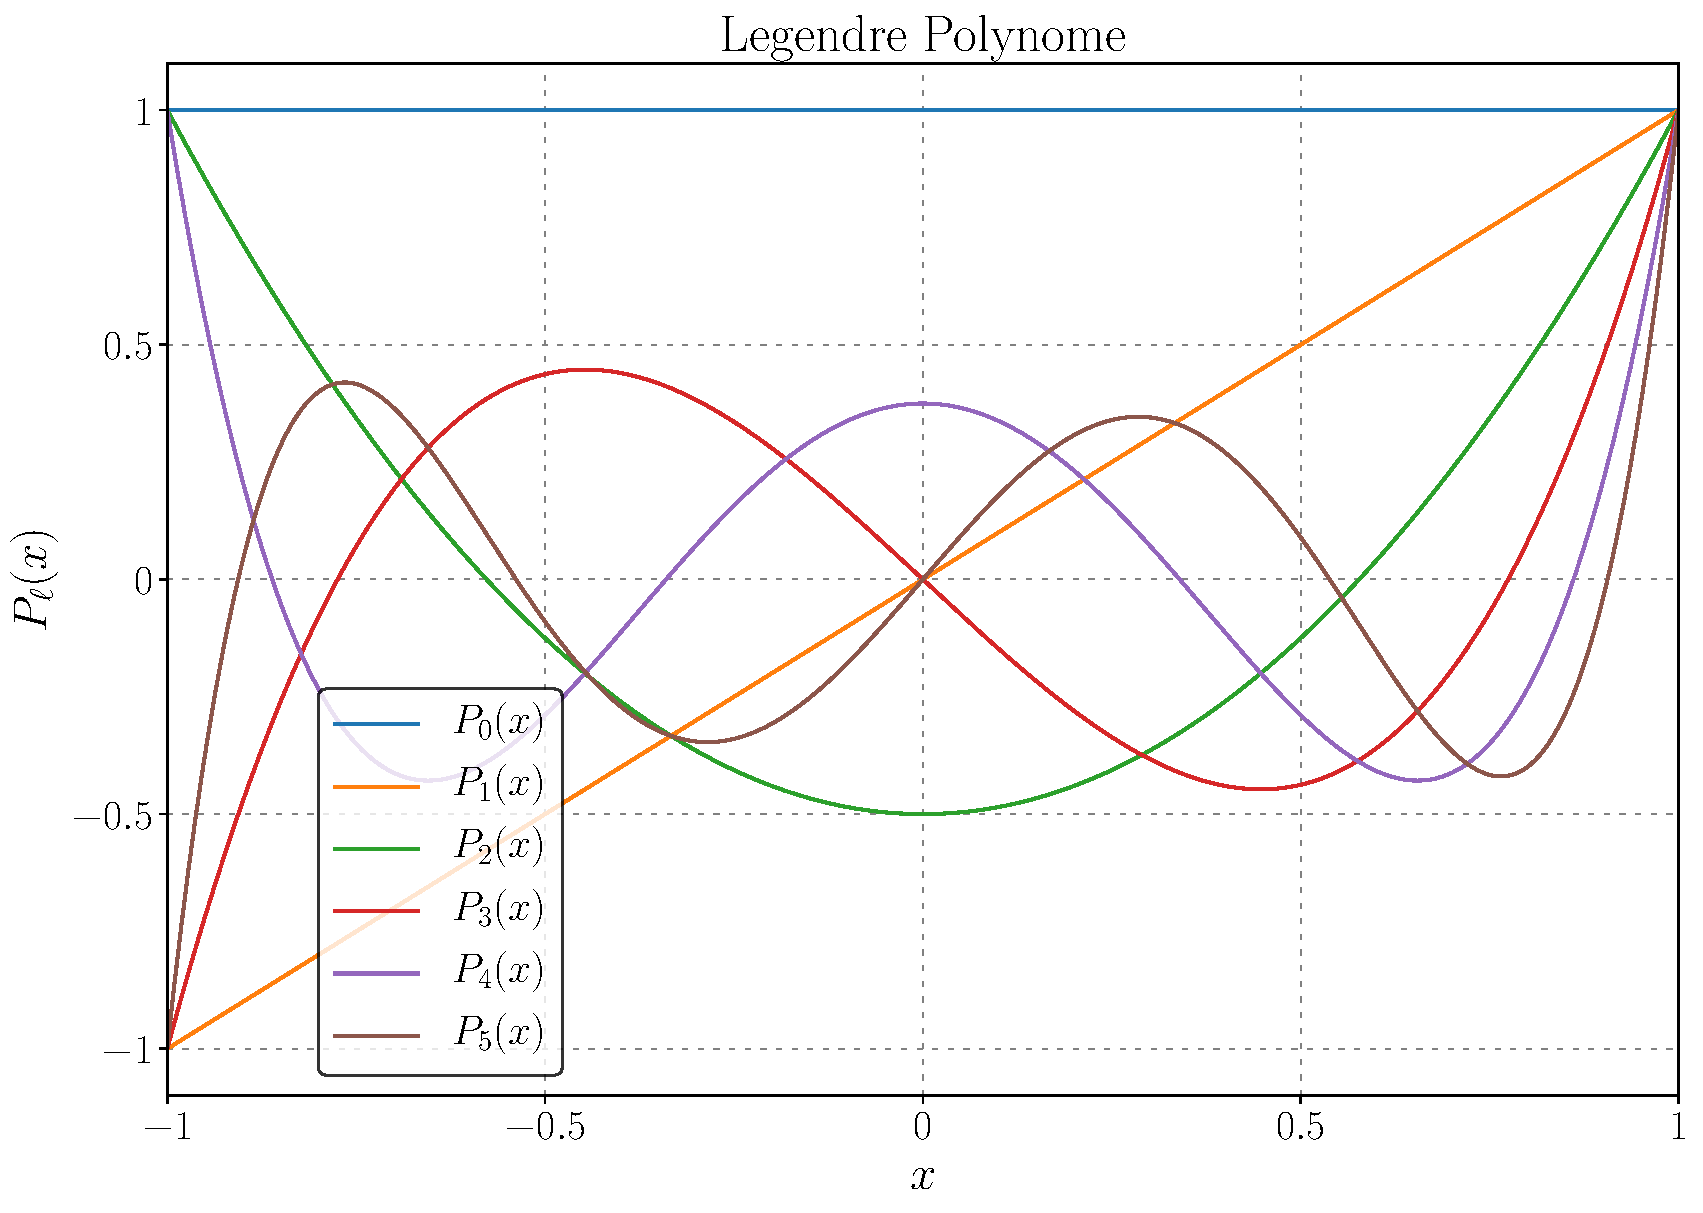
\includegraphics[width=10cm]{1-Legendre-Polynome.pdf}
\caption{Die ersten sechs Legendre-Polynome}
\end{figure}

\begin{figure}[h]
\centering
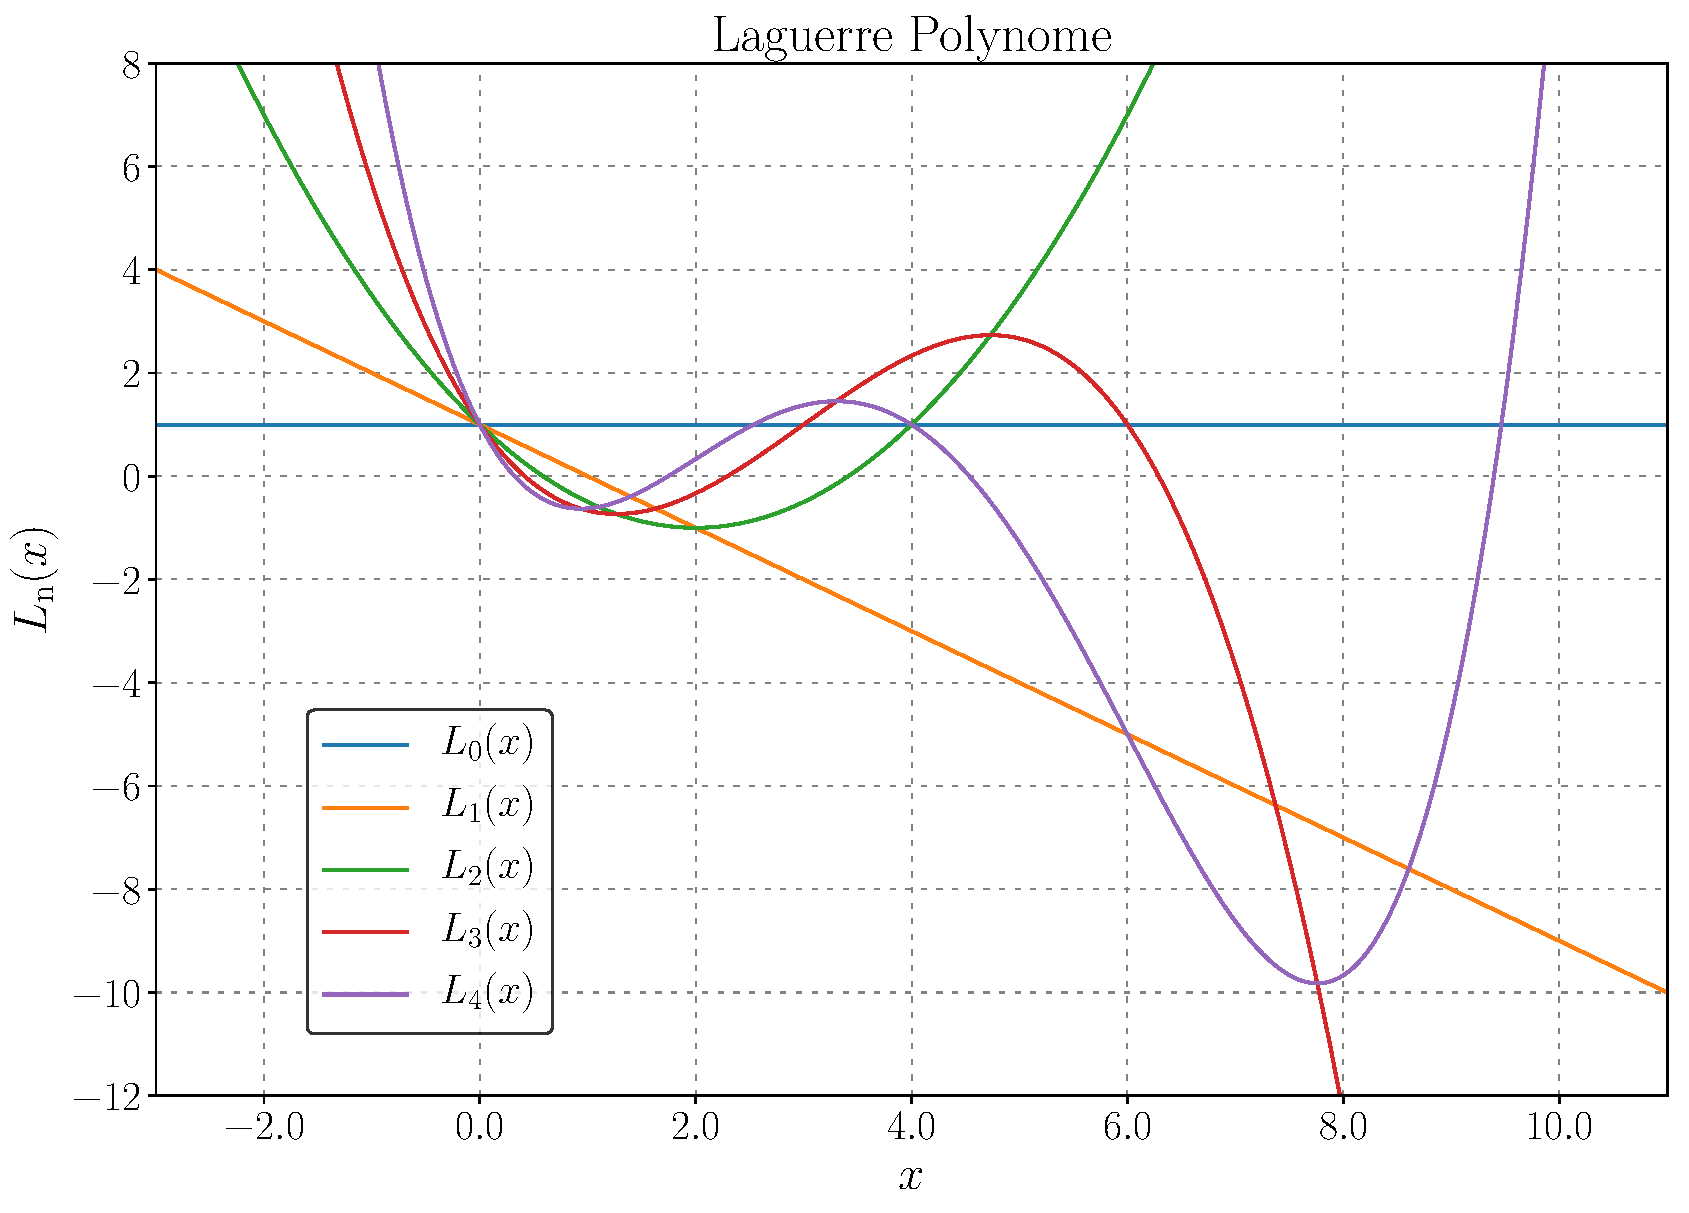
\includegraphics[width=10cm]{2-Laguerre-Polynome.pdf}
\caption{Die ersten fünf Laguerre-Polynome}
\end{figure}

\begin{figure}[h]
\centering
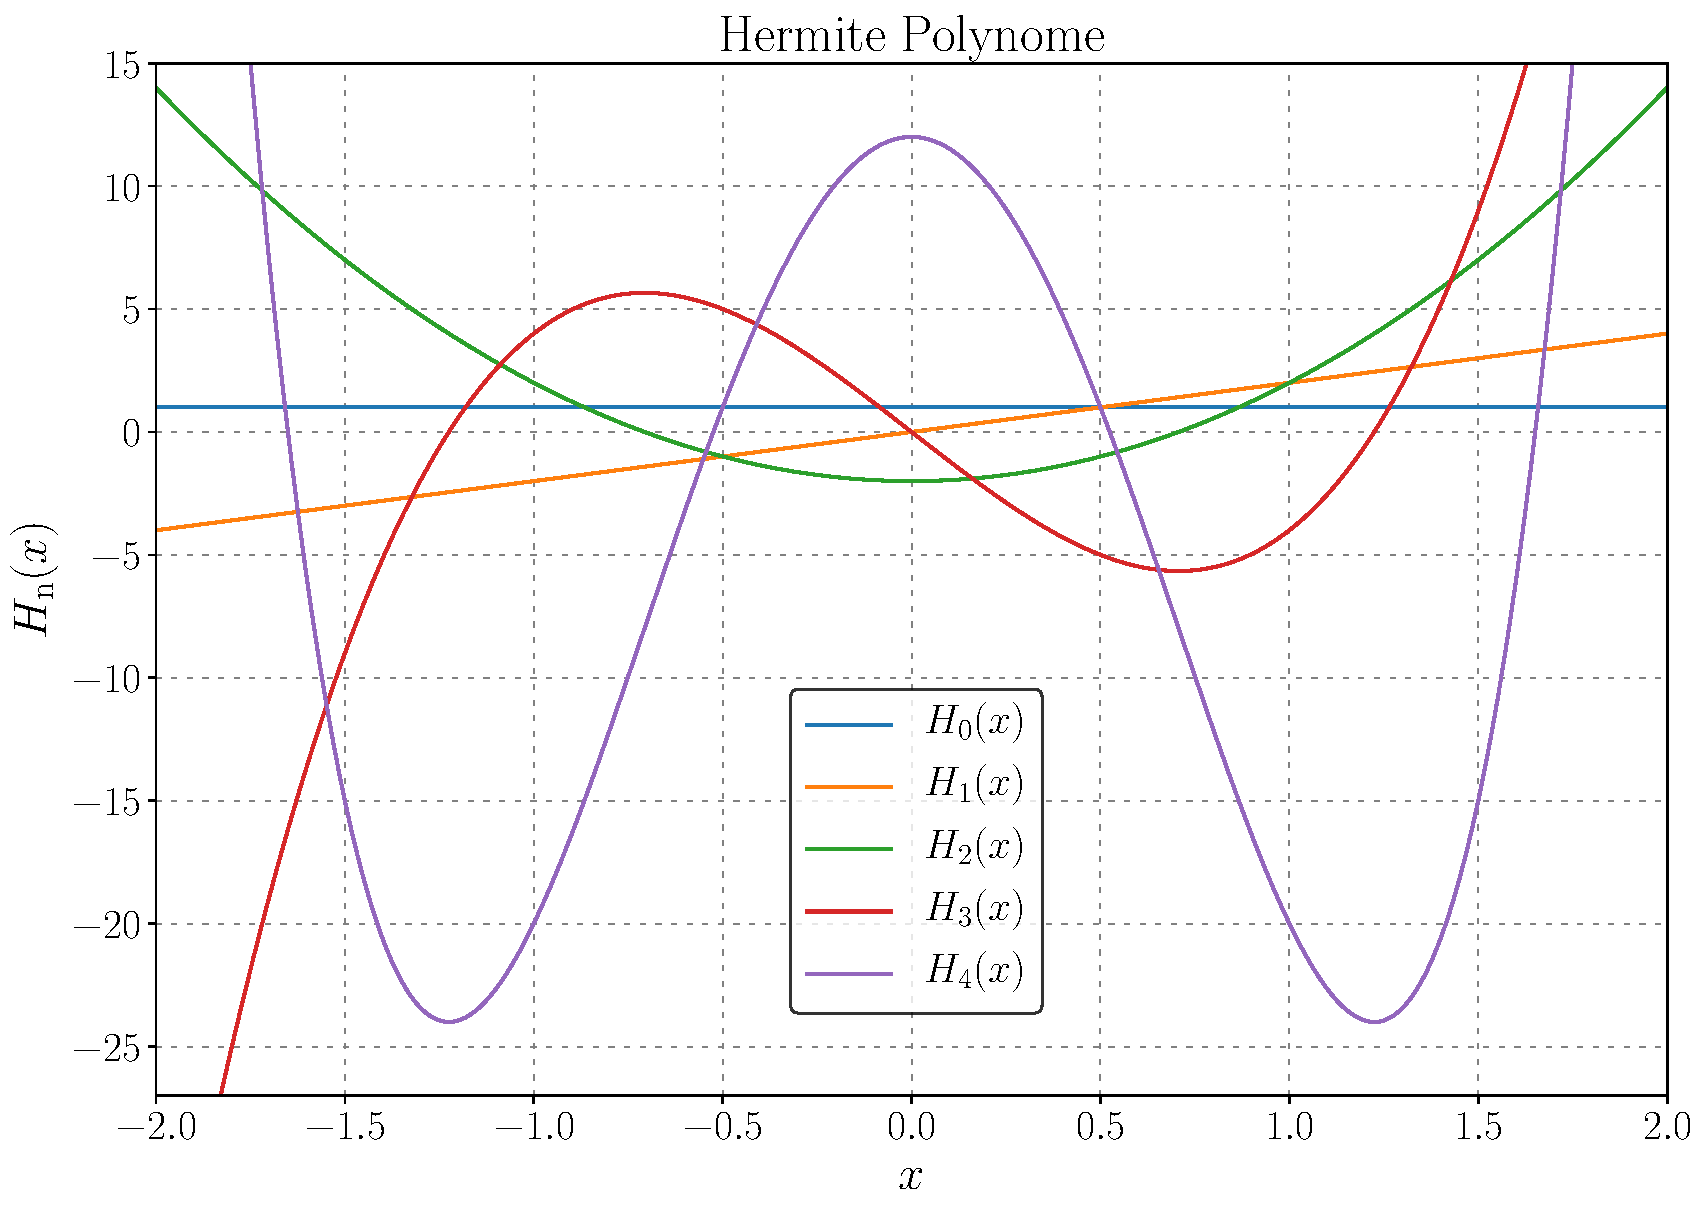
\includegraphics[width=10cm]{3-Hermite-Polynome.pdf}
\caption{Die ersten fünf Hermite-Polynome}
\end{figure}

Die ersten neun Legendre-Polynome lauten:
\\[0.3cm]
\renewcommand{\arraystretch}{1.4}
\begin{tabular*}{1.00\textwidth}{>{\RaggedRight}p{3cm}>{\RaggedRight}p{7cm}} \hline
\textbf{$\ell$}  &\textbf{$P_{\ell}(x)$} \\ \hline\hline
0 & $1$ \\
1 & $x$ \\
2 & $\frac{1}{2}(3x^2-1)$ \\
3 & $\frac{1}{2}x(5x^2-3)$ \\
4 & $\frac{1}{8}(35x^4-30x^2+3)$ \\
5 & $\frac{1}{8}x(63x^4-70x^2+15)$ \\
6 & $\frac{1}{16}(231x^6-315x^4+105x^2-5)$ \\
7 & $\frac{1}{16}x(429x^6-693x^4+315x^2-35)$ \\
8 & $\frac{1}{128}(6435x^8-12012x^6+6930x^4-1260x^2+35)$ \\ \hline
\end{tabular*}

\newpage
\subsubsection{Lösung des Radialanteils}


\subsection{Lösung des Radialanteils}

\subsection{Darstellung und Visualisierung der Gesamtlösungen}
















\newpage
\chapter{Nonrelativistic Many-Electron Theory}


\section{Spin Angular Momentum}

\subsection{Lie Groups and Lie Algebras}
\url{https://de.wikipedia.org/wiki/Wigner-Eckart-Theorem}\\
\url{https://en.wikipedia.org/wiki/Wigner%E2%80%93Eckart_theorem}\\
\url{https://en.wikipedia.org/wiki/Tensor_operator}

\subsection{Angular Momentum Operators}

\subsection{Ladder Operator Method}
Allgemein gilt, dass jeder Vektoroperator, der die Kommutatorrelationen
\begin{equation}
[\hat{J}_x,\hat{J}_y]=\mathrm{i}\hbar\hat{J}_z\;,\qquad\quad[\hat{J}_y,\hat{J}_z]=\mathrm{i}\hbar\hat{J}_x\;,\qquad\quad[\hat{J}_z,\hat{J}_x]=\mathrm{i}\hbar\hat{J}_y
\end{equation}
sowie
\begin{equation}
[\hat{\vec{J}}^{\;2},\hat{J}_x]=0\;,\qquad\quad[\hat{\vec{J}}^{\;2},\hat{J}_y]=0\;,\qquad\quad[\hat{\vec{J}}^{\;2},\hat{J}_z]=0\label{commutator}
\end{equation}
erfüllt und dessen Komponenten hermitesch sind,
\begin{equation}
\big(\hat{\vec{J}}^{\;2}\big)^{\dagger}=\hat{\vec{J}}^{\;2}\;,\qquad\hat{J}^{\dagger}_{x}=\hat{J}_{x}\;,\qquad\hat{J}^{\dagger}_{y}=\hat{J}_{y}\;,\qquad\hat{J}^{\dagger}_{z}=\hat{J}_{z}\;,
\end{equation}
als Drehimpuls bezeichnet wird. Im Folgenden sollen aus den fundamentalen Kommutatorrelationen des Drehimpulsoperators und der Hermitezität seine Eigenwerte und Eigenfunktionen bestimmt werden. \eqref{commutator} sagt aus, dass $\hat{\vec{J}}^{\;2}$ und die drei Komponenten von $\hat{\vec{J}}$ kommutierende Observablen sind. Wenn wir als Komponente $\hat{J}_z$ wählen, dann besitzen die hermiteschen, kommutierenden Operatoren $\hat{\vec{J}}^{\;2}$ und $\hat{J}_z$ simultane Eigenzustände mit reellen, aber unterschiedlichen Eigenwerten, die wir mit $\lambda$ und $m$ bezeichnen:
\begin{align}
\hat{\vec{J}}^{\;2}|\lambda,m\rangle &= \lambda|\lambda,m\rangle\label{Eigenwert1}\\
\hat{J}_{z}|\lambda,m\rangle &= m|\lambda,m\rangle\label{Eigenwert2}
\end{align}
Für einen hermiteschen Operator gilt:
\begin{equation}
\langle\psi|\hat{O}^{2}|\psi\rangle\geq 0
\end{equation}
Daraus lassen sich Informationen über die Eigenwerte von $\hat{\vec{J}}^{\;2}$ und $\hat{J}_z$ extrahieren:
\begin{alignat*}{2}
&\qquad           & \hat{\vec{J}}^{\;2} &= \hat{J}_{x}^{2}+\hat{J}_{y}^{2}+\hat{J}_{z}^{2}         \\
&\Leftrightarrow     &  \hat{\vec{J}}^{\;2}-\hat{J}_{z}^{2}     &= \hat{J}_{x}^{2}+\hat{J}_{y}^{2}        \\
&\Leftrightarrow  & \hat{\vec{J}}^{\;2}-\hat{J}_{z}^{2} &=          \lambda -m^2\\
&\Leftrightarrow  & \big(\hat{\vec{J}}^{\;2}-\hat{J}_{z}^{2}\big)\big|\lambda,m\big\rangle &= \big(\lambda-m^2\big)\big|\lambda,m\big\rangle         \\
&\Leftrightarrow     &  \big\langle\lambda,m\big|\hat{\vec{J}}^{\;2}-\hat{J}_{z}^{2}\big|\lambda,m\big\rangle     &=  \big(\lambda-m^2\big)\langle\lambda,m|\lambda,m\rangle \\
&\Leftrightarrow     &  \big\langle\lambda,m\big|\hat{\vec{J}}^{\;2}-\hat{J}_{z}^{2}\big|\lambda,m\big\rangle    &=    \big(\lambda-m^2\big)
\end{alignat*}
Daraus folgt
\begin{equation}
\lambda\geq m^2\geq 0\label{Abbruchbedingung}
\end{equation}
Jetzt werden die Leiteroperatoren
\begin{equation}
\hat{J}_{+}=\hat{J}_{x}+\mathrm{i}\hat{J}_{y}\qquad\mathrm{und}\qquad\hat{J}_{-}=\hat{J}_{x}-\mathrm{i}\hat{J}_{y}
\end{equation}
eingeführt. Hierfür gelten die Kommutatorrelationen
\begin{equation}
[\hat{J}_{+},\hat{J}_{z}]=-\hat{J}_{+}\;,\qquad [\hat{J}_{-},\hat{J}_{z}]=\hat{J}_{-}\;,\qquad [\hat{J}_{+},\hat{J}_{-}]=2\hat{J}_{z}\;,\qquad [\hat{\vec{J}}^{\;2},\hat{J}_{\pm}]=0
\end{equation}
Ähnlich wie bei der Behandlung des harmonischen Oszillators werden die Leiteroperatoren in die Eigenwertgleichungen \eqref{Eigenwert1} und \eqref{Eigenwert2} eingeschoben:
\begin{equation}
\hat{\vec{J}}^{\;2}\hat{J}_{\pm}\big|\lambda,m\big\rangle = \hat{J}_{\pm}\hat{\vec{J}}^{\;2}\big|\lambda,m\big\rangle = \lambda\hat{J}_{\pm}\big|\lambda,m\big\rangle
\end{equation}
und
\begin{align}
\hat{J}_{z}\hat{J}_{\pm}\big|\lambda,m\big\rangle &= \big(\hat{J}_{\pm}\hat{J}_{z}-[\hat{J}_{\pm},\hat{J}_{z}]\big)\big|\lambda,m\rangle\\
&= \big(\hat{J}_{\pm}\hat{J}_{z}\pm\hat{J}_{\pm}\big)\big|\lambda,m\rangle\\
&= \hat{J}_{\pm}\hat{J}_{z}\big|\lambda,m\big\rangle\pm\hat{J}_{\pm}\big|\lambda,m\big\rangle\\
&= (m\pm 1)\hat{J}_{\pm}\big|\lambda,m\big\rangle
\end{align}
Ein Einschieben des Operators $\hat{J}_{\pm}$ in die Eigenwertgleichung für $\hat{J}_{z}$ führt also zur Erhöhung oder Erniedrigung des Eigenwertes um 1. Einschieben von $\hat{J}_{\pm}$ in die Eigenwertgleichung für $\hat{\vec{J}}^{\;2}$ führt dagegen zu einer Beibehaltung des Eigenwertes. Zusammenfassend erhält man:
\begin{equation}
\hat{J}_{\pm}\big|\lambda,m\big\rangle = c_{\pm}\big|\lambda,m\pm 1\big\rangle\label{Zustandsentwicklung}
\end{equation}
Die Faktoren $c_{\pm}$ erhält man wie beim harmonischen Oszillator über die Normierung. Dafür wird noch die Beziehung
\begin{equation}
\hat{\vec{J}}^{\;2}=\hat{J}_{x}^{2}+\hat{J}_{y}^{2}+\hat{J}_{z}^{2}=\hat{J}_{+}\hat{J}_{-}+\hat{J}_{z}^{2}-\hat{J}_{z}
\end{equation}
benötigt. Für den Absteigeoperator ergibt das
\begin{align}
|c_{-}|^{2} &= \big\langle\lambda,m\big|\hat{J}_{+}\hat{J}_{-}\big|\lambda,m\big\rangle\\
&= \big\langle\lambda,m\big|\hat{\vec{J}}^{\;2}-\hat{J}_{z}^{2}+\hat{J}_{z}\big|\lambda,m\big\rangle\\
&= \lambda-m^{2}+m
\end{align}
Für den Aufsteigeoperator erhält man
\begin{align}
|c_{+}|^{2} &= \big\langle\lambda,m\big|\hat{J}_{-}\hat{J}_{+}\big|\lambda,m\big\rangle\\
&= \big\langle\lambda,m\big|\hat{\vec{J}}^{\;2}-\hat{J}_{z}^{2}-\hat{J}_{z}\big|\lambda,m\big\rangle\\
&= \lambda-m^{2}-m
\end{align}
und damit insgesamt
\begin{equation}
c_{-}=\sqrt{\lambda-m(m-1)}\;,\qquad\quad c_{+}=\sqrt{\lambda-m(m+1)}
\end{equation}
Aus \eqref{Zustandsentwicklung} erhält man durch Anwenden von $\hat{J}_{\pm}$ sukzessive die Zustände mit anderen $m$-Werten,
\begin{equation}
|\lambda,m\rangle,\qquad|\lambda,m\pm 1\rangle,\qquad|\lambda,m\pm 2\rangle,\qquad ...\label{Zustandsfolge}
\end{equation}
Wegen \eqref{Abbruchbedingung} muss diese Zustandsfolge abbrechen. Das geschieht nur, wenn die Faktoren $c_{\pm}$ gleich 0 werden. Es müssen also $m_{\mathrm{max}}$ und $m_{\mathrm{min}}$ existieren, sodass gilt:
\begin{equation}
\lambda=m_{\mathrm{max}}(m_{\mathrm{max}}+1)\qquad\mathrm{und}\qquad\lambda=m_{\mathrm{min}}(m_{\mathrm{min}}-1)\label{m-Werte}
\end{equation}
Durch Einführen eines Zusatzterms und Umformung erhält man
\begin{equation}
(m_{\mathrm{max}}+m_{\mathrm{min}})(m_{\mathrm{max}}-m_{\mathrm{min}}+1)=0
\end{equation}
Es gilt natürlich $m_{\mathrm{max}}\geq m_{\mathrm{min}}$, sodass die zweite Klammer immer ungleich null ist. Daher muss die erste Klammer null ergeben. Daraus folgt direkt
\begin{equation}
m_{\mathrm{max}}=-m_{\mathrm{min}}=j,\qquad j\geq 0
\end{equation}
Für den Eigenwert $\lambda$ folgt aus \eqref{m-Werte}, dass nur bestimmte Werte
\begin{equation}
\lambda = j(j+1)
\end{equation}
möglich sind. Da die Folge \eqref{Zustandsfolge} abbricht, muss der Aufsteigeoperator $\hat{J}_{+}$ von $m_{\mathrm{min}}=-j$ zu $m_{\mathrm{max}}=j$ führen. Daher sind für gegebenes $j$ die folgenden $m$-Werte möglich:
\begin{equation}
m=-j,\;-j+1,\;-j+2,\;...\;,\;j-2,\;j-1,\;j\label{Drehimpulsquantenzahlen}
\end{equation}
Aus dieser Folge möglicher $m$-Werte ergibt sich, dass sich die Strecke von $-j$ bis $j$ in Schritte der Größe $\Delta m=1$ aufteilen lassen muss. Das funktioniert nur für ganz- oder halbzahlige $j$-Werte. Damit sind auch die $m$-Werte ganz- oder halbzahlig. Der Eigenwert $\lambda$ wird im Ket-Vektor $|\lambda,m\rangle$ üblicherweise durch die Drehimpulsquantenzahl $j$ ersetzt, da die Angabe aller Quantenzahlen eines Systems seine Zustände vollständig beschreibt:
\begin{equation}
|\lambda,m\rangle\quad\Rightarrow\quad|j,m\rangle
\end{equation}
Die Eigenwertprobleme für den Drehimpuls lauten damit
\begin{align}
\hat{\vec{J}}^{\;2}|j,m\rangle &= j(j+1)|j,m\rangle\label{Eigenwertergebnis 1}\\
\hat{J}_{z}|j,m\rangle &= m|j,m\rangle\label{Eigenwertergebnis 2}
\end{align}
Ähnlich wie beim Harmonischen Oszillator können jetzt durch $n$-fache Anwendung von $\hat{J}_{+}$ bzw. $\hat{J}_{-}$ bei gegebenem $j$ die Zustände $|j,-j\rangle$ bis $|j,j\rangle$ sowie die zugehörigen Koeffizienten bestimmt werden:
\begin{align}
\hat{J}_{-}^{\;n}|j,j\rangle = c_{-}(j,j)|j,j-n\rangle\qquad &\Rightarrow\qquad\langle j,j|\hat{J}_{+}^{\;n} = \langle j,j-n|c_{-}^{*}(j,j)\\
\hat{J}_{+}^{\;n}|j,-j\rangle = c_{+}(j,j)|j,-j+n\rangle\qquad &\Rightarrow\qquad\langle j,-j|\hat{J}_{-}^{\;n} = \langle j,-j+n|c_{+}^{*}(j,j)
\end{align}
Die Werte für die Koeffizienten erhält man wie gewohnt über die Normierungsbedingung:
\begin{align}
1=\langle j,j-n|j,j-n\rangle &= \frac{1}{|c_{-}(j,j)|^2}\big\langle j,j\big|\hat{J}_{+}^{\;n}\hat{J}_{-}^{\;n}\big|j,j\big\rangle\\
\mathrm{oder}\qquad 1=\langle j,-j+n|-j+n\rangle &= \frac{1}{|c_{+}(j,j)|^2}\big\langle j,-j\big|\hat{J}_{-}^{\;n}\hat{J}_{+}^{\;n}\big|j,-j\big\rangle
\end{align}





\subsection{Spin-Lösungen}
Aus \eqref{Drehimpulsquantenzahlen} folgte, dass nur ganz- oder halbzahlige $j$-Werte (Drehimpulsquantenzahlen) möglich sind. Halbzahlige Drehimpulsquantenzahlen charakterisieren einen Drehimpuls, der sich vom Bahndrehimpuls unterscheidet und der \textit{Spin} oder Eigendrehimpuls genannt wird. Ausgehend vom allgemeinen Eigenzustand $|j,m\rangle$ wird ein Bezeichnungswechsel zu $|s,s_{z}\rangle$ durchgeführt. Für Fermionen gilt immer $s=\frac{1}{2}$. Daraus folgt direkt, dass nur zwei $"$Spinrichtungen$"$ möglich sind, die mit
\begin{equation}
\bigg|\frac{1}{2},\frac{1}{2}\bigg\rangle=\big|\uparrow\big\rangle\qquad\mathrm{und}\qquad\bigg|\frac{1}{2},-\frac{1}{2}\bigg\rangle=\big|\downarrow\big\rangle
\end{equation}
bezeichnet werden. Ähnlich wie für den Bahndrehimpuls wird auch für den Spin ein Spinoperator
\begin{equation}
\hat{\vec{S}}=
\renewcommand{\arraystretch}{1.2}
\left(\begin{array}{c} \hat{S}_{x} \\ \hat{S}_{y} \\ \hat{S}_{z} \\\end{array}\right)
\end{equation}
eingeführt. Als Drehimpuls erfüllt der Spin die Kommutatorrelationen
\begin{align}
[\hat{\vec{S}}^{\,2},\hat{S}_{i}] &= 0 \\
[\hat{S}_{x},\hat{S}_{y}] &= \mathrm{i}\hbar\hat{S}_{z} \\
[\hat{S}_{y},\hat{S}_{z}] &= \mathrm{i}\hbar\hat{S}_{x} \\
[\hat{S}_{z},\hat{S}_{x}] &= \mathrm{i}\hbar\hat{S}_{y}
\end{align}
sowie die Eigenwertgleichungen
\begin{align}
\hat{\vec{S}}^{\,2}|s,s_{z}\rangle &= \hbar^{2}s(s+1)|s,s_{z}\rangle\\
\hat{S}_{z}|s,s_{z}\rangle &= \hbar s_{z}|s,s_{z}\rangle
\end{align}
Zuerst sollen die Eigenfunktionen von $\hat{\vec{S}}^{\,2}$ bzw. $\hat{S}_{z}$ durch Übergang in die Matrixschreibweise ermittelt werden. Auch für den Spin sind die Matrixelemente durch \eqref{Eigenwertergebnis 1} und \eqref{Eigenwertergebnis 2} festgelegt:
\begin{align}
\big\langle s,s_{z}'\big|\hat{\vec{S}}^{\;2}\big|s,s_{z}\big\rangle &= \hbar^{2}s(s+1)\delta_{s_{z}s_{z}'}
\\
\big\langle s,s_{z}'\big|\hat{S}_{z}\big|s,s_{z}\big\rangle &= \hbar \,s_{z}\,\delta_{s_{z}s_{z}'}
\\
\big\langle s,s_{z}'\big|\hat{S}_{+}\big|s,s_{z}\big\rangle &= \hbar\sqrt{(s-s_{z})(s+s_{z}+1)}\,\delta_{s_{z}'s_{z}+1}
\\
\big\langle s,s_{z}'\big|\hat{S}_{-}\big|s,s_{z}\big\rangle &= \hbar\sqrt{(s+s_{z})(s-s_{z}+1)}\,\delta_{s_{z}'s_{z}-1}
\end{align}
Die obigen Operatoren werden in der $\{\big|\uparrow\big\rangle,\big|\downarrow\big\rangle\}$-Basis durch $2\times 2$-Matrizen dargestellt:
\begin{equation}
\renewcommand{\arraystretch}{1.4}
\hat{S}_{i}:=
\left(\begin{array}{cc}
\big\langle \uparrow\big|\hat{S}_i\big|\uparrow\big\rangle
&
\big\langle \uparrow\big|\hat{S}_i\big|\downarrow\big\rangle
\\
\big\langle \downarrow\big|\hat{S}_i\big|\uparrow\big\rangle
& 
\big\langle \downarrow\big|\hat{S}_i\big|\downarrow\big\rangle
\\\end{array}\right)
\end{equation}
Die Berechnung der Matrixelemente liefert
\begin{align}
\renewcommand{\arraystretch}{1.1}
\hat{\vec{S}}^{\,2}:=
\frac{3}{4}\hbar^{2}\left(\begin{array}{cc}
1
&
0
\\
0
& 
1
\\\end{array}\right) &\;;\qquad
\renewcommand{\arraystretch}{1.1}
\hat{S}_{z}:=
\frac{\hbar}{2}\left(\begin{array}{cc}
1
&
0
\\
0
& 
-1
\\\end{array}\right)
\\
\renewcommand{\arraystretch}{1.1}
\hat{S}_{+}:=
\hbar\left(\begin{array}{cc}
0
&
1
\\
0
& 
0
\\\end{array}\right) &\;;\qquad
\renewcommand{\arraystretch}{1.1}
\hat{S}_{-}:=
\hbar\left(\begin{array}{cc}
0
&
0
\\
1
& 
0
\\\end{array}\right)
\\
\hat{S}_{x}=\frac{1}{2}\big(\hat{S}_{+}+&\hat{S}_{-}\big):=\frac{\hbar}{2}
\renewcommand{\arraystretch}{1.1}
\left(\begin{array}{cc}
0
&
1
\\
1
& 
0
\\\end{array}\right)
\\
\hat{S}_{y}=\frac{1}{2\mathrm{i}}\big(\hat{S}_{+}-&\hat{S}_{-}\big):=\frac{\hbar}{2}
\renewcommand{\arraystretch}{1.1}
\left(\begin{array}{cc}
0
&
-\mathrm{i}
\\
\mathrm{i}
& 
0
\\\end{array}\right)
\end{align}




\subsection{Die SU(2)-Drehgruppe}










\subsection{Kopplung von Drehimpulsen}
Es sollen zwei Drehimpulse $\hat{\vec{J}}_1$ und $\hat{\vec{J}}_2$ betrachtet werden. Der Zustandsraum für den Drehimpuls $\hat{\vec{J}}_1$ mit der Dimension $2j_1+1$ sei der endlichdimensionale Hilbertraum $\mathcal{H}_1$. Dann ist der Zustandsraum für den Drehimpuls $\hat{\vec{J}}_2$ mit der Dimension $2j_2+1$ durch den Hilbertraum $\mathcal{H}_2$ gegeben. Der gemeinsame Zustandsraum für beide Drehimpulse ist das Tensorprodukt der Hilberträume der einzelnen Drehimpulse
\begin{equation}
\mathcal{H}=\mathcal{H}_1\otimes\mathcal{H}_2
\end{equation}
mit der Dimension $(2j_1+1)(2j_2+1)$. Um den Gesamtdrehimpulsoperator $\hat{\vec{J}}$ zu bilden, muss beachtet werden, dass $\hat{\vec{J}}_1$ auf $\mathcal{H}_1$ und $\hat{\vec{J}}_2$ auf $\mathcal{H}_2$ wirkt. Daraus folgt, dass $\hat{\vec{J}}$ auf $\mathcal{H}_1\otimes\mathcal{H}_2$ wirken muss. Bevor der Gesamtdrehimpulsoperator aus der Summe der Einzeldrehimpulsoperatoren zusammengesetzt werden kann, müssen $\hat{\vec{J}}_1$ und $\hat{\vec{J}}_2$ auf $\mathcal{H}$ erweitert werden. Das geschieht, indem das Tensorprodukt von $\hat{\vec{J}}_1$ ($\hat{\vec{J}}_2$) mit dem Einsoperator auf $\mathcal{H}_2$ ($\mathcal{H}_1$) gebildet wird:
\begin{equation}
\hat{\vec{J}}=\hat{\vec{J}}_{1}\otimes\mathbbm{1}+\mathbbm{1}\otimes\hat{\vec{J}}_{2}\label{Hilbertraum-Erweiterung}
\end{equation}
Als Basis für Drehimpulszustände, die sich aus zwei einzelnen Drehimpulsen zusammensetzen, bietet sich die Eigenbasis zu $\{\hat{\vec{J}}_{1}^{\,2},\hat{J}_{1z},\hat{\vec{J}}_{2}^{\,2},\hat{J}_{2z}\}$ an, da alle Operatoren miteinander kommutieren und sie einen vollständigen Satz kommutierender Observablen bilden. Da die Einzeldrehimpulse auf unterschiedliche Freiheitsgrade wirken, sind die Eigenzustände dann durch die Tensorproduktzustände
\begin{equation}
\big|j_{1},m_{1};j_{2},m_{2}\big\rangle = \big|j_{1},m_{1}\big\rangle\otimes \big|j_{2},m_{2}\big\rangle\label{uncoupled_states}
\end{equation}
gegeben. Es gilt
\begin{alignat*}{3}
[\hat{\vec{J}}_{1}^{\,2},\hat{\vec{J}}_{2}^{\,2}] &= 0\qquad\quad
[\hat{\vec{J}}_{1}^{\,2},\hat{J}_{1z}] &= 0\qquad\quad
[\hat{\vec{J}}_{1}^{\,2},\hat{J}_{2z}] &= 0\\
[\hat{J}_{1z},\hat{\vec{J}}_{2}^{\,2}] &= 0\qquad\quad
[\hat{J}_{1z},\hat{J}_{2z}] &= 0\qquad\quad
[\hat{\vec{J}}_{2}^{\,2},\hat{J}_{2z}] &= 0
\end{alignat*}
Die Zustände \eqref{uncoupled_states} werden auch als ungekoppelte Zustände bezeichnet. Sie beschreiben ein System aus zwei Drehimpulsen, die nicht miteinander wechselwirken. Diese Zustände erfüllen die Eigenwertgleichungen
\begin{alignat*}{3}
\hat{\vec{J}}_{1}^{\,2}\; & \big|j_1,m_1;j_1,m_2\big\rangle = & \;j_1(j_1+1)\hbar^2\; & \big|j_1,m_1;j_2,m_2\big\rangle \\
\hat{J}_{1z} & \big|j_1,m_1;j_1,m_2\big\rangle = & m_1\hbar\; & \big|j_1,m_1;j_2,m_2\big\rangle \\
\hat{\vec{J}}_{2}^{\,2}\; & \big|j_1,m_1;j_1,m_2\big\rangle = & \;j_2(j_2+1)\hbar^2\; & \big|j_1,m_1;j_2,m_2\big\rangle \\
\hat{J}_{2z} & \big|j_1,m_1;j_1,m_2\big\rangle = & m_2\hbar\; & \big|j_1,m_1;j_2,m_2\big\rangle
\end{alignat*}
In der Realität koppeln Einzeldrehimpulse allerdings zu einem Gesamtdrehimpuls. Die zu dieser Eigenbasis gehörenden Operatoren bilden den vollständigen Satz kommutierender Observablen $\{\hat{\vec{J}}_{1}^{\,2},\hat{\vec{J}}_{2}^{\,2},\hat{\vec{J}}^{\,2},\hat{J}_{z}\}$. Sie erfüllen die Kommutatorrelationen
\begin{alignat*}{3}
[\hat{\vec{J}}^{\,2},\hat{J}_{z}] &= 0\qquad\quad
[\hat{\vec{J}}^{\,2},\hat{\vec{J}}_{1}^{\,2}] &= 0\qquad\quad
[\hat{\vec{J}}^{\,2},\hat{\vec{J}}_{2}^{\,2}] &= 0\\
[\hat{J}_{z},\hat{\vec{J}}_{1}^{\,2}] &= 0\qquad\quad
[\hat{J}_{z},\hat{\vec{J}}_{2}^{\,2}] &= 0\qquad\quad
[\hat{\vec{J}}_{1}^{\,2},\hat{\vec{J}}_{2}^{\,2}] &= 0
\end{alignat*}
und die Eigenwertgleichungen
\begin{alignat*}{5}
\hat{\vec{J}}_{1}^{\,2}\; & \big|j_1,j_2,J,M\big\rangle = & \;j_1(j_1+1)\hbar^2\; & \big|j_1,j_2,J,M\big\rangle \\
\hat{\vec{J}}_{2}^{\,2}\; & \big|j_1,j_2,J,M\big\rangle = & \;j_2(j_2+1)\hbar^2\; & \big|j_1,j_2,J,M\big\rangle \\
\hat{\vec{J}}^{\,2}\; & \big|j_1,j_2,J,M\big\rangle = & \;J(J+1)\hbar^2\; & \big|j_1,j_2,J,M\big\rangle \\
\hat{J}_{z}\; & \big|j_1,j_2,J,M\big\rangle = & M\hbar\; & \big|j_1,j_2,J,M\big\rangle
\end{alignat*}
Die ungekoppelten Zustände \eqref{uncoupled_states} können zwar über Tensorproduktbildung leicht aus den Zuständen zu den Einzeldrehimpulsen erhalten werden. Für die zum Gesamtdrehimpuls gekoppelten Zustände $\big|j_1,j_2,J,M\big\rangle$ gilt das aber nicht. Man kann sich aber zunutze machen, dass beide Eigenbasen $\{\big|j_1,m_1;j_2,m_2\big\rangle\}$ und $\{\big|j_1,j_2,J,M\big\rangle\}$ Orthonormalbasen bilden.





\subsection{Clebsch-Gordan-Koeffizienten}
Man kann daher die die neuen Basiszustände $\{\big|j_1,j_2,J,M\big\rangle\}$ nach den alten Basiszuständen $\{\big|j_1,m_1;j_2,m_2\big\rangle\}$ entwickeln:
\begin{equation}
\big|j_1,j_2,J,M\big\rangle = \sum_{m_1=-j_1}^{j_1}\sum_{m_2=-j_2}^{j_2}\big|j_1,m_1;j_2,m_2\big\rangle\big\langle j_1,m_1;j_2,m_2\big|j_1,j_2,J,M\big\rangle\label{Clebsch-Gordan-Reihe}
\end{equation}
Wendet man $\hat{J}_{z}$ auf diese Zustände an, ergibt sich
\begin{equation}
\hat{J}_{z}\big|j_1,j_2,J,M\big\rangle = M\hbar\big|j_1,j_2,J,M\big\rangle
\end{equation}
Da gleichzeitig
\begin{equation}
\big(\hat{J}_{1z}+\hat{J}_{2z}\big)\big|j_1,j_2,J,M\big\rangle = (m_1+m_2)\hbar\big|j_1,j_2,J,M\big\rangle
\end{equation}
gelten muss, ergibt sich daraus
\begin{equation}
M = m_1+m_2
\end{equation}
Damit lässt sich jetzt der erste Zustand \eqref{Clebsch-Gordan-Reihe} für die größten möglichen Werte für $m_1$ und $m_2$ bestimmen. Daraus ergibt sich der größte mögliche Wert für $M$, der zugleich der größte Wert für $J$ ist:
\begin{equation}
M_{\mathrm{max}}=j_1+j_2 = J_{\mathrm{max}}
\end{equation}
Daher besteht die Clebsch-Gordan-Reihe aus nur einem Beitrag:
\begin{equation}
\big|j_1,j_2,J,M\big\rangle = \sum_{m_1,m_2}C\big|j_1,m_1;j_2,m_2\big\rangle =\big|j_1,j_1\big\rangle\otimes\big|j_2,j_2\big\rangle
\end{equation}
wobei der erste Clebsch-Gordan-Koeffizient willkürlich auf 1 gesetzt wurde. Die weiteren Zustände können jetzt berechnet werden, indem der Absteigeoperator $\hat{J}_{-}=\hat{J}_{1-}+\hat{J}_{2-}$ auf den ersten Zustand angewendet wird:
\begin{align}
\hat{J}_{-}\big|j_1+j_2,j_1,j_2,j_1+j_2\big\rangle &= \big(\hat{J}_{1-}+\hat{J}_{2-}\big)\big|j_1,j_1\big\rangle\otimes\big|j_2,j_2\big\rangle\\
&=\hat{J}_{1-}\big(\big|j_1,j_1\big\rangle\otimes\big|j_2,j_2\big\rangle\big)+\hat{J}_{2-}\big(\big|j_1,j_1\big\rangle\otimes\big|j_2,j_2\big\rangle\big)\\
&=\big(\hat{J}_{1-}\big|j_1,j_1\big\rangle\big)\otimes\big|j_2,j_2\big\rangle+\big|j_1,j_1\big\rangle\otimes\big(\hat{J}_{2-}\big|j_2,j_2\big\rangle\big)
\end{align}
Außerdem gilt für den Absteigeoperator:
\begin{equation}
\hat{J}_{-}\big|J,M\big\rangle = \sqrt{J(J+1)-M(M-1)}\hbar\big|J,M-1\big\rangle\label{Absteigeoperator}
\end{equation}
Wenn man $\hat{J}_{-}$ auf $\big|j_1+j_2,j_1,j_2,j_1+j_2\big\rangle$ unter Ausnutzung von \eqref{Absteigeoperator} anwendet, ergibt sich
\begin{align}
\hat{J}_{-}\big|j_1+j_2,j_1,j_2,j_1+j_2\big\rangle &= \sqrt{(j_1+j_2)(j_1+j_2+1)-(j_1+j_2)(j_1+j_2-1)}\big|j_1+j_2,j_1,j_2,j_1+j_2-1\big\rangle\notag\\
&= \sqrt{(j_1+j_2)(j_1+j_2+1-j_1-j_2+1)}\big|j_1+j_2,j_1,j_2,j_1+j_2-1\big\rangle\notag\\
&= \sqrt{2(j_1+j_2)}\big|j_1+j_2,j_1,j_2,j_1+j_2-1\big\rangle
\end{align}
Die Anwendung von $\hat{J}_{-}$ auf $\big|j_1,j_1\big\rangle\otimes\big|j_2,j_2\big\rangle$ ergibt:
\begin{align}
\hat{J}_{-}\big|j_1,j_1\big\rangle\otimes\big|j_2,j_2\big\rangle&= \big(\hat{J}_{1-}\big|j_1,j_1\big\rangle\big)\otimes\big|j_2,j_2\big\rangle + \big|j_1,j_1\big\rangle\otimes\big(\hat{J}_{2-}\big|j_2,j_2\big\rangle\big)\\
&= \sqrt{j_1(j_1+1)-j_1(j_1-1)}\big|j_1,j_1-1\big\rangle\otimes\big|j_2,j_2\big\rangle\notag\\
&\quad +\sqrt{j_2(j_2+1)-j_2(j_2-1)}\big|j_2,j_2-1\big\rangle\otimes\big|j_1,j_1\big\rangle\\
&= \sqrt{2j_1}\big|j_1,j_1-1\big\rangle\otimes\big|j_2,j_2\big\rangle+\sqrt{2j_2}\big|j_2,j_2-1\big\rangle\otimes\big|j_1,j_1\big\rangle
\end{align}
Zusammengenommen ergibt das:
\begin{align}
\sqrt{2(j_1+j_2)}&\big|j_1+j_2,j_1,j_2,j_1+j_2-1\big\rangle\\
&=\sqrt{2j_1}\big|j_1,j_1-1\big\rangle\otimes\big|j_2,j_2\big\rangle+\sqrt{2j_2}\big|j_2,j_2-1\big\rangle\otimes\big|j_1,j_1\big\rangle
\end{align}











\newpage
\subsection{Spin-Spin-Kopplung}
Im Folgenden wird das Konstruktionsverfahren zur Bestimmung der gekoppelten Zustände auf die Kopplung zweier Spins $s_1$ und $s_2$ zum Gesamtspin $S$ angewendet. Es wird die Notation
\begin{equation}
j_1 = s_1 = \frac{1}{2},\qquad j_2 = s_2 = -\frac{1}{2},\qquad J = S,\qquad M = M
\end{equation}
verwendet. Die ungekoppelten Basiszustände sind gegeben durch
\begin{equation}
\renewcommand{\arraystretch}{1.6}
\big|s_1,m_1;s_2,m_2\big\rangle=\left\{\begin{array}{ccc} \big|\frac{1}{2},\frac{1}{2}\big\rangle\otimes\big|\frac{1}{2},\frac{1}{2}\big\rangle&=&\left|\uparrow\uparrow\right\rangle\\
\big|\frac{1}{2},\frac{1}{2}\big\rangle\otimes\big|\frac{1}{2},-\frac{1}{2}\big\rangle&=&\left|\uparrow\downarrow\right\rangle\\
\big|\frac{1}{2},-\frac{1}{2}\big\rangle\otimes\big|\frac{1}{2},\frac{1}{2}\big\rangle&=&\left|\downarrow\uparrow\right\rangle\\
\big|\frac{1}{2},-\frac{1}{2}\big\rangle\otimes\big|\frac{1}{2},-\frac{1}{2}\big\rangle&=&\left|\downarrow\downarrow\right\rangle\\ \end{array}\right.
\end{equation}


\section{Pauli Principle}

\section{Second Quantization}

\section{Configuration State Functions (CSFs)}
Die elektronische Schrödingergleichung liefert nicht die exakten elektronischen Energien und Eigenzustände eines Systems, da sie relativistische Effekte wie den Elektronenspin und die damit zusammenhängenden Energiebeiträge vernachlässigt. Die relativistische Erweiterung der Schrödingergleichung ist die Dirac-Gleichung. Daher wirkt der Hamiltonoperator der Schrödingergleichung nicht auf den Spin, sodass die Kommutatorrelationen
\begin{equation}
[\hat{H}_{\mathrm{el}},\hat{\vec{S}}^{\,2}]=0,\qquad[\hat{H}_{\mathrm{el}},\hat{S}_{z}]=0,\qquad[\hat{\vec{S}}^{\,2},\hat{S}_{z}]=0\label{commutation-relations}
\end{equation}
gelten. Hierbei sei $\hat{H}_{\mathrm{el}}$ der molekulare elektronische Hamiltonoperator eines Mehrelektronensystems im Coulombpotential mehrerer Atomkerne. Das impliziert, dass $\hat{\vec{S}}^{\,2}$ und $\hat{S}_{z}$ die Operatoren zum Gesamtspin des Systems sein müssen. Die zugehörigen Spinzustände sind die zum Gesamtspin gekoppelten Zustände $|S,M\rangle$, die über die Clebsch-Gordan-Koeffizienten berechnet werden können. Sie spannen den endlichdimensionalen Hilbertraum
\begin{equation}
\mathcal{H}_{\mathrm{S}}=\bigotimes_{i=1}^{N}\mathbb{C}_{i}^{2}
\end{equation}
auf, wobei $N$ die Anzahl der Elektronen ist. $\mathbb{C}_{i}^{2}$ ist der Spinorraum des $i$-ten Elektrons. Zwar bilden auch die ungekoppelten Spinzustände eine Orthonormalbasis dieses Vektorraums, allerdings sind in der Realität die Spins miteinander wechselwirkender Elektronen immer gekoppelt. Das vom Spin ausgehende magnetische Moment und andere damit zusammenhängende relativistische Effekte wie die Spin-Bahn-Kopplung haben oft nur einen kleinen Einfluss auf die Gesamtenergie. Trotzdem haben die Spinzustände $|S,M\rangle$ alleine aufgrund ihrer Symmetrieeigenschaften einen großen Einfluss auf die elektronische Struktur von Atomen, wie in den nächsten Abschnitten deutlich wird. Um den Spin zu berücksichtigen, kann die Gesamtwellenfunktion in einem ersten Ansatz als Tensorprodukt
\begin{equation}
|\Phi_n\rangle = |\psi_n\rangle\otimes|S,M\rangle\label{Gesamtwellenfunktion}
\end{equation}
geschrieben werden, wobei $|\psi_n\rangle$ den reinen Ortszustand bezeichnet. Die Kommutatorrelationen \eqref{commutation-relations} rechtfertigen diesen Ansatz. Der Hilbertraum des Gesamtsystems ist gegeben durch
\begin{equation}
\mathcal{H}=\mathcal{H}_{\mathrm{K}}\otimes\mathcal{H}_{\mathrm{S}}=\bigg(\bigotimes_{i=1}^{N}L^{2}(\mathbb{R}^{3})_{i}\bigg)\otimes\bigg(\bigotimes_{i=1}^{N}\mathbb{C}_{i}^{2}\bigg)
\end{equation}
Aus \eqref{commutation-relations} kann man außerdem ableiten, dass die Gesamtwellenfunktion den folgenden Eigenwertgleichungen genügen muss:
\begin{align}
\hat{H}_{\mathrm{el}}|\Phi_n\rangle &= E_n |\Phi_n\rangle \\
\hat{\vec{S}}^{\,2}|\Phi_n\rangle &= S(S+1)\hbar^{2}|\Phi_n\rangle \\
\hat{S}_{z}|\Phi_n\rangle &= M\hbar|\Phi_n\rangle
\end{align}
Die Operatoren des Gesamtspins müssen natürlich auf den Spinorraum eines $N$-Elektronensystems erweitert werden. Dies geschieht analog zu \eqref{Hilbertraum-Erweiterung} durch das folgende Verfahren:
\begin{align}
\hat{\vec{S}}^{\,2} &= \bigg(\Big(\big(\hat{\vec{S}}_{1}^{\,2}\otimes\hat{\mathbbm{1}}+\hat{\mathbbm{1}}\otimes\hat{\vec{S}}_{2}^{\,2}\big)\otimes\hat{\mathbbm{1}}+\hat{\mathbbm{1}}\otimes\hat{\mathbbm{1}}\otimes\hat{\vec{S}}_{3}^{\,2}\Big)\cdots\bigg)\otimes\hat{\mathbbm{1}}+\bigg(\bigotimes_{i=1}^{N-1}\hat{\mathbbm{1}}_{i}\bigg)\otimes\hat{\vec{S}}_{N}^{\,2} \\
\hat{S}_{z} &= \bigg(\Big(\big(\hat{S}_{1z}\otimes\hat{\mathbbm{1}}+\hat{\mathbbm{1}}\otimes\hat{S}_{2z}\big)\otimes\hat{\mathbbm{1}}+\hat{\mathbbm{1}}\otimes\hat{\mathbbm{1}}\otimes\hat{S}_{3z}\Big)\cdots\bigg)\otimes\hat{\mathbbm{1}}+\bigg(\bigotimes_{i=1}^{N-1}\hat{\mathbbm{1}}_{i}\bigg)\otimes\hat{S}_{Nz}
\end{align}
Das Tensorprodukt ist auf endlichdimensionalen Räumen durch das Kroneckerprodukt gegeben. Der $\hat{\mathbbm{1}}$-Operator ist definiert als
\begin{equation}
\hat{\mathbbm{1}}=\sum_{j=1}^{2}\big|s,s_{jz}\big\rangle\big\langle s,s_{jz}\big|=\left|\uparrow\right\rangle\langle\left\uparrow\right|+\left|\downarrow\right\rangle\langle\left\downarrow\right|
\end{equation}
Eine wichtige Erkenntnis dieses Abschnitts ist, dass die Wellenfunktion $|\Phi_n\rangle$ nur dann mit Sicherheit Eigenfunktion von $\hat{\vec{S}}^{\,2}$ und $\hat{S}_{z}$ ist, wenn der Spinanteil separabel ist, also in der Form \eqref{Gesamtwellenfunktion} vorliegt. Dass dies nicht selbstverständlich ist, wird im nächsten Abschnitt deutlich.




\section{Hartree-Fock Approximation}

\subsection{Schalennäherung}
Der Hamiltonoperator für ein Mehrelektronensystem in Born-Oppenheimer-Näherung (ohne Kern-Kern-Wechselwirkung) lautet:
\begin{equation}
\hat{H}_{\mathrm{el}}=\sum_{i=1}^{N}\underbrace{\bigg(\frac{\hbar^2}{2m_i}\nabla_{i}^{2}+\frac{1}{4\pi\varepsilon_0}\sum_{\alpha=1}^{K}\frac{Z_{\alpha}e^2}{\Vert\vec{r}_{i}-\vec{R}_{\alpha}\Vert}\bigg)}_{\hat{h}_{i}}+\frac{1}{4\pi\varepsilon_0}\sum_{j=1}^{N}\sum_{i<j}^{N}\frac{e^2}{\Vert\vec{r}_{i}-\vec{r}_{j}\Vert}
\end{equation}
Wenn die Elektron-Elektron-Repulsion vernachlässigt wird, reduziert sich der Hamiltonoperator zu einer Summe aus Einelektronen-Operatoren:
\begin{equation}
\hat{H}_{\mathrm{el}}=\sum_{i=1}^{N}\hat{h}_{i}
\end{equation}
Jeder Einelektronen-Operator $\hat{h}_{i}$ hat Eigenzustände der Form
\begin{equation}
|\xi_a\rangle_i =|\phi_a\rangle_i\otimes|s,s_{z}\rangle
\end{equation}
Die elektronische Schrödingergleichung kann damit geschrieben werden als
\begin{equation}
\sum_{i=1}^{N}\hat{h}_{i}|\Phi_{n}\rangle=E_{n}|\Phi_{n}\rangle
\end{equation}
mit
\begin{equation}
|\Phi_{n}\rangle=\bigotimes_{i=1}^{N}|\xi_{a_i}\rangle_i\qquad\mathrm{und}\qquad E_{n}=\sum_{i=1}^{N}\varepsilon_{a_i}
\end{equation}
Diese Produktwellenfuktionen werden Hartree-Produkte genannt. Betrachtet man ein Zweielektronensystem, so bewirkt die Ununterscheidbarkeit der Elektronen aber, dass das Hartree-Produkt $|\xi_{a_1}\rangle_1\otimes|\xi_{a_2}\rangle_2$ noch eine weitere, äquivalente Realisierungsmöglichkeit besitzt, nämlich $|\xi_{a_1}\rangle_2\otimes|\xi_{a_2}\rangle_1$. Ein einzelnes Hartree-Produkt ist nicht antisymmetrisch unter Vertauschung zweier Elektronen, was das Pauli-Prinzip aber verlangt. Eine Linearkombination beider Hartree-Produkte von der Form
\begin{equation}
|\Phi_{n}\rangle = \frac{1}{\sqrt{2}}\Big(|\xi_{a_1}\rangle_1\otimes|\xi_{a_2}\rangle_2 - |\xi_{a_1}\rangle_2\otimes|\xi_{a_2}\rangle_1\Big)
\end{equation}
erfüllt dagegen die Antisymmetrie-Bedingung und ist gleichzeitig Eigenzustand von $\hat{H}_{\mathrm{el}}$. Der Vorfaktor sorgt für die Normierung. Diese Wellenfunktion kann in Form einer Determinante geschrieben werden:
\begin{equation}
|\Phi_{n}\rangle = \frac{1}{\sqrt{2}}\begin{array}{|cc|}
|\xi_{a_1}\rangle_1  &  |\xi_{a_2}\rangle_1 \\
|\xi_{a_1}\rangle_2  &  |\xi_{a_2}\rangle_2 \\
\end{array}
\end{equation}
Diese sogenannte Slater-Determinante kann auf $N$ Elektronen verallgemeinert werden:
\begin{equation}
|\Phi_{n}\rangle = \frac{1}{\sqrt{N!}}\begin{array}{|ccccc|}
|\xi_{a_1}\rangle_1  &  |\xi_{a_2}\rangle_1  &  |\xi_{a_3}\rangle_1  & \cdots  &  |\xi_{a_N}\rangle_1 \\
|\xi_{a_1}\rangle_2  &  |\xi_{a_2}\rangle_2  &  |\xi_{a_3}\rangle_2  & \cdots  &  |\xi_{a_N}\rangle_2 \\
|\xi_{a_1}\rangle_3  &  |\xi_{a_2}\rangle_3  &  |\xi_{a_3}\rangle_3  & \cdots  &  |\xi_{a_N}\rangle_3 \\
\vdots  &  \vdots  &  \vdots  & \ddots  &  \vdots \\
|\xi_{a_1}\rangle_N  &  |\xi_{a_2}\rangle_N  &  |\xi_{a_3}\rangle_N  & \cdots  &  |\xi_{a_N}\rangle_N\\
\end{array}
\end{equation}
Äquivalent dazu kann die Slater-Determinante dadurch definiert werden, dass ein Antisymmetrisierungsoperator $\hat{A}$ auf das $N$-fache Hartree-Produkt angewendet wird:
\begin{equation}
|\Phi_{n}\rangle = \hat{A}\bigotimes_{i=1}^{N}|\xi_{a_i}\rangle_i = \frac{1}{\sqrt{N!}}\sum_{\sigma=1}^{N!}\mathrm{sgn}(\sigma)\bigotimes_{i=1}^{N}|\xi_{a_i}\rangle_i
\end{equation}
Der Ausdruck auf der rechten Seite ist die Leibniz-Formel zur Determinantenberechnung. Dafür werden zuerst alle Permutationen der zugrundeliegenden Matrix bestimmt. Sei $X=\{x_1, x_2,...,x_n\}$ eine Menge mit $N$ Elementen, in diesem Fall die Menge der Matrixspalten, dann ist eine $N$-stellige Permutation ohne Wiederholung eine bijektive Abbildung
\begin{equation}
\sigma:X\to X,
\end{equation}
die jedem Element der Menge ein Element der gleichen Menge zuordnet. In der ausführlichen Darstellung einer $N$-stelligen Permutation schreibt man diese als Matrix mit zwei Zeilen und $N$ Spalten. In der oberen Zeile stehen die Zahlen von 1 bis $N$ (in beliebiger Reihenfolge). Unter jeder Zahl steht dann in der zweiten Zeile der Funktionswert $\sigma(i)$, also ein Spaltenindex der Matrix:
\begin{equation}
\sigma=\left(\begin{array}{cccc}
1  &  2  &  \cdots  &  N  \\
\sigma(1)  &  \sigma(2)  &  \cdots  & \sigma(n)
\end{array}\right)
\end{equation}
Die Anzahl der möglichen Permutationen von $N$ Objekten wird durch die Fakultät $N!$ angegeben. Für den Fall eines Dreielektronensystems ergeben sich zum Beispiel $3!=6$ Permutationen:
\begin{table}[H]
	\begin{center}
		%\renewcommand{\arraystretch}{2.6}
		\begin{tabular}{cccc}
			\hline
			Nr.  &  $\sigma$  &  $\mathrm{sgn}(\sigma)$  &  $\displaystyle\bigotimes_{i=1}^{N}\big|\xi_{a_{\sigma(i)}}\big\rangle_i $
			\\ \hline\hline
			1  &
			$\left(\begin{array}{ccc}1  &  2  &  3  \\ 1  &  2  &  3  \\\end{array}\right)$  &
			$+$  &
			$|\xi_{a_1}\rangle_1\otimes|\xi_{a_2}\rangle_2\otimes|\xi_{a_3}\rangle_3$
			\\
			2  &
			$\left(\begin{array}{ccc}1  &  2  &  3  \\ 1  &  3  &  2  \\\end{array}\right)$  &
			$-$  &
			$|\xi_{a_1}\rangle_1\otimes|\xi_{a_3}\rangle_2\otimes|\xi_{a_2}\rangle_3$
			\\
			3  &
			$\left(\begin{array}{ccc}1  &  2  &  3  \\ 2  &  1  &  3  \\\end{array}\right)$  &
			$-$  &
			$|\xi_{a_2}\rangle_1\otimes|\xi_{a_1}\rangle_2\otimes|\xi_{a_3}\rangle_3$
			\\
			4  &
			$\left(\begin{array}{ccc}1  &  2  &  3  \\ 2  &  3  &  1  \\\end{array}\right)$  &
			$+$  &
			$|\xi_{a_2}\rangle_1\otimes|\xi_{a_3}\rangle_2\otimes|\xi_{a_1}\rangle_3$
			\\
			5  &
			$\left(\begin{array}{ccc}1  &  2  &  3  \\ 3  &  1  &  2  \\\end{array}\right)$  &
			$+$  &
			$|\xi_{a_3}\rangle_1\otimes|\xi_{a_1}\rangle_2\otimes|\xi_{a_2}\rangle_3$
			\\
			6  &
			$\left(\begin{array}{ccc}1  &  2  &  3  \\ 3  &  2  &  1  \\\end{array}\right)$  &
			$-$  &
			$|\xi_{a_3}\rangle_1\otimes|\xi_{a_2}\rangle_2\otimes|\xi_{a_1}\rangle_3$
			\\\hline
		\end{tabular}
	\end{center}
\end{table}
Um eine korrekte elektronische Wellenfunktion $|\Phi_n\rangle$ zu erhalten, muss aber noch sichergestellt werden, dass diese nicht nur Eigenfunktion zu $\hat{H}_{\mathrm{el}}$ ist, sondern auch Eigenfunktion zu $\hat{\vec{S}}^{\,2}$ und $\hat{S}_z$. Aufgrund der Spinwellenfunktion $|s,s_z\rangle$, die zwei Einstellungsmöglichkeiten hat, können aus einem Ortsorbital $|\phi_a\rangle$ zwei Spinorbitale $|\xi_{a_1}\rangle$ und $|\xi_{a_2}\rangle$ gebildet werden. Für ein Zweielektronensystem im Grundzustand ergibt das:
\begin{align}
|\Phi_0\rangle &= \frac{1}{\sqrt{2}}\Big(|\xi_1\rangle_1\otimes|\xi_2\rangle_2 - |\xi_1\rangle_2\otimes|\xi_2\rangle_1\Big)\\
&= \frac{1}{\sqrt{2}}\Big(|\phi_1\rangle_1\otimes\big|\tfrac{1}{2},\tfrac{1}{2}\big\rangle_1\otimes|\phi_1\rangle_2\otimes\big|\tfrac{1}{2},-\tfrac{1}{2}\big\rangle_2 - |\phi_1\rangle_2\otimes\big|\tfrac{1}{2},\tfrac{1}{2}\big\rangle_2\otimes|\phi_1\rangle_1\otimes\big|\tfrac{1}{2},-\tfrac{1}{2}\big\rangle_1\Big)\\
&= \big|\phi_1\big\rangle_1\big|\phi_1\big\rangle_2\frac{1}{\sqrt{2}}\Big(\big|\tfrac{1}{2},\tfrac{1}{2}\big\rangle_1\otimes\big|\tfrac{1}{2},-\tfrac{1}{2}\big\rangle_2 - \big|\tfrac{1}{2},\tfrac{1}{2}\big\rangle_2\otimes\big|\tfrac{1}{2},-\tfrac{1}{2}\big\rangle_1\Big)\\
&= \big|\phi_1\big\rangle_1\big|\phi_1\big\rangle_2\frac{1}{\sqrt{2}}\big(\left|\uparrow\downarrow\right\rangle - \left|\downarrow\uparrow\right\rangle\big)
\end{align}
In diesem Fall ist die Spinwellenfunktion in der Determinante also separabel und damit Eigenfunktion der Spinoperatoren. Es handelt sich wenig überraschend um einen Singulett-Zustand. Man kann zeigen, dass jede Slater-Determinante mit einer geraden Zahl von Elektronen, in der alle Ortsorbitale doppelt besetzt sind (\textit{restricted closed-shell}-Konfiguration), in dieser Weise separabel ist und damit Eigenfunktion der Spinoperatoren ist.



\subsection{Herleitung}
Die Hartree-Fock-Näherung ist eine ab initio-Methode zur näherungsweisen Lösung der elektronischen Schrödingergleichung, in der die molekulare Grundzustandswellenfunktion als Slater-Determinante aus Einelektronenwellenfunktionen angesetzt wird. Für die folgende Herleitung wird die Ortsdarstellung verwendet, in der die Slater-Determinante die Form
\begin{equation}
\Phi_{0}(\vec{r}_1,...,\vec{r}_N,s_1,...,s_N) = \frac{1}{\sqrt{N!}}\begin{array}{|cccc|}
\xi_{1}(\vec{r}_1)  &  \xi_{2}(\vec{r}_1)    & \cdots  &  \xi_{N}(\vec{r}_1) \\
\xi_{1}(\vec{r}_2)  &  \xi_{2}(\vec{r}_2)    & \cdots  &  \xi_{N}(\vec{r}_2) \\
\vdots  &  \vdots    & \ddots  &  \vdots \\
\xi_{1}(\vec{r}_N)  &  \xi_{2}(\vec{r}_N)    & \cdots  &  \xi_{N}(\vec{r}_N)\\
\end{array}
\end{equation}
annimmt. Die Hartree-Fock-Grundzustandsenergie lautet mit dem Slater-Determinanten-Ansatz:
\begin{align}
E_{0}&=\big\langle\Phi_{0}\big|\hat{H}_{\mathrm{el}}\big|\Phi_{0}\big\rangle\\
&=\bigg\langle\Phi_{0}\bigg|\sum_{i=1}^{N}\hat{h}_{i}+\frac{1}{4\pi\varepsilon_0}\sum_{j=1}^{N}\sum_{i<j}^{N}\frac{e^2}{\Vert\hat{r}_{i}-\hat{r}_{j}\Vert}\bigg|\Phi_{0}\bigg\rangle\\
&=\sum_{i=1}^{N}\big\langle\Phi_{0}\big|\hat{h}_{i}\big|\Phi_{0}\big\rangle +\frac{e^2}{4\pi\varepsilon_0}\sum_{j=1}^{N}\sum_{i<j}^{N}\Big\langle\Phi_{0}\Big|\frac{1}{\Vert\hat{r}_{i}-\hat{r}_{j}\Vert}\Big|\Phi_{0}\Big\rangle
\end{align}
Zuerst soll der erste Term durch Einsetzen der Slater-Determinante in Ortsdarstellung ausgewertet werden:
\begin{align}
\sum_{i=1}^{N}\big\langle\Phi_{0}\big|\hat{h}_{i}\big|\Phi_{0}\big\rangle &= \frac{1}{N!}\sum_{i=1}^{N}\Bigg[\int\cdots\int\bigg(\sum_{\sigma=1}^{N!}\mathrm{sgn}(\sigma)\prod_{j=1}^{N}\xi_{\sigma(j)}^{*}(\vec{r}_{j})\bigg)\hat{h}_{i}\bigg(\sum_{\nu=1}^{N!}\mathrm{sgn}(\nu)\prod_{k=1}^{N}\xi_{\nu(k)}(\vec{r}_{k})\bigg)\prod_{l=1}^{N}\mathrm{d}^{3}r_{l}\Bigg]\notag\\
&=\frac{1}{N!}\sum_{i=1}^{N}\Bigg[\int\cdots\int\sum_{\sigma=1}^{N!}\sum_{\nu=1}^{N!}\mathrm{sgn(\sigma)}\mathrm{sgn(\nu)}\prod_{j=1}^{N}\xi_{\sigma(j)}^{*}(\vec{r}_{j})\hat{h}_{i}\prod_{k=1}^{N}\xi_{\nu(k)}(\vec{r}_{k})\prod_{l=1}^{N}\mathrm{d}^{3}r_{l}\Bigg]\notag\\
&=\frac{1}{N!}\sum_{i=1}^{N}\sum_{\sigma=1}^{N!}\sum_{\nu=1}^{N!}\mathrm{sgn(\sigma)}\mathrm{sgn(\nu)}\int\cdots\int\prod_{j=1}^{N}\xi_{\sigma(j)}^{*}(\vec{r}_{j})\hat{h}_{i}\prod_{k=1}^{N}\xi_{\nu(k)}(\vec{r}_{k})\prod_{l=1}^{N}\mathrm{d}^{3}r_{l}\notag\\
&=\frac{1}{N!}\sum_{i=1}^{N}\sum_{\sigma=1}^{N!}\int\cdots\int\,\xi_{\sigma(i)}^{*}(\vec{r}_{i})\hat{h}_{i}\xi_{\sigma(i)}(\vec{r}_{i})\prod_{l=1}^{N}\mathrm{d}^{3}r_{l}\notag\\
&=\frac{1}{N!}\sum_{i=1}^{N}N!\int\xi_{\sigma}^{*}(\vec{r}_{i})\hat{h}_{i}\xi_{\sigma}(\vec{r}_{i})\mathrm{d}^{3}r_{i}=\sum_{i=1}^{N}\big\langle\xi_{\sigma}\big|\hat{h}_i\big|\xi_{\sigma}\big\rangle=\sum_{\sigma=1}^{N}\big\langle\xi_{\sigma}\big|\hat{h}\big|\xi_{\sigma}\big\rangle\notag
\end{align}
Damit ergibt sich schlussendlich ein Energieausdruck für die Hartree-Fock-Energie:
\begin{align}
E_{0}[\{\xi_{\sigma}\}]&=\sum_{\sigma=1}^{N}\int\xi_{\sigma}^{*}(\vec{r}_i)\hat{h}_{i}\xi_{\sigma}(\vec{r}_i)\mathrm{d}^3r_i +\frac{1}{2}\sum_{\sigma=1}^{N}\sum_{\mu=1}^{N}\bigg(\iint\xi_{\sigma}^{*}(\vec{r}_i)\xi_{\mu}^{*}(\vec{r}_j)\hat{w}_{ij}\xi_{\sigma}(\vec{r}_i)\xi_{\mu}(\vec{r}_j)\mathrm{d}^3r_i\mathrm{d}^3r_j\notag\\
&\qquad\qquad\qquad\qquad\qquad\qquad -\iint\xi_{\sigma}^{*}(\vec{r}_i)\xi_{\mu}^{*}(\vec{r}_j)\hat{w}_{ij}\xi_{\mu}(\vec{r}_i)\xi_{\sigma}(\vec{r}_j)\mathrm{d}^3r_i\mathrm{d}^3r_j\bigg)\\
&=\sum_{\sigma=1}^{N}\langle\xi_{\sigma}|\hat{h}|\xi_{\sigma}\rangle +\frac{1}{2}\sum_{\sigma=1}^{N}\sum_{\mu=1}^{N}\big(\langle\xi_{\sigma}\xi_{\mu}|\hat{w}|\xi_{\sigma}\xi_{\mu}\rangle - \langle\xi_{\sigma}\xi_{\mu}|\hat{w}|\xi_{\mu}\xi_{\sigma}\rangle\big)
\end{align}
Um die Hartree-Fock-Gleichungen herzuleiten, muss der Energieausdruck $E_{0}[\{\xi_{\sigma}\}]$ minimiert werden, wozu das Verfahren der Lagrange-Multiplikatoren verwendet wird. Unter der Nebenbedingung
\begin{equation}
\int\xi_{\sigma}^{*}(\vec{r}_1)\xi_{\mu}(\vec{r}_1)\mathrm{d}^3r_1 = \big\langle\xi_{\sigma}\big|\xi_{\mu}\big\rangle = \delta_{\sigma\mu}
\end{equation}
ist das Lagrange-Funktional $\mathcal{L}[\{\xi_{\sigma}\}]$ definiert als
\begin{equation}
\mathcal{L}[\{\xi_{\sigma}\}]
\end{equation}




\subsection{Roothan-Hall-Gleichungen}
Durch die Eliminierung des Spins bleibt eine Hartree-Fock-Gleichung der Form
\begin{equation}
\hat{f}|\phi_i\rangle = \varepsilon_i|\phi_i\rangle
\end{equation}
übrig, die eine Eigenwertgleichung in der Form einer Integro-Differentialgleichung ist. Die Molekülorbitale $|\phi_i\rangle$ können durch einen Basissatz
\begin{equation}
|\phi_i\rangle = \sum_{\nu=1}^{K}|\varphi_{\nu}\rangle\langle\varphi_{\nu}|\phi_i\rangle = \sum_{\nu=1}^{K}C_{\nu i}|\varphi_{\nu}\rangle
\end{equation}
entwickelt werden. Einsetzen in die Hartree-Fock-Gleichung und Multiplikation von links mit $\langle\varphi_{\mu}|$ liefert:
\begin{equation}
\sum_{\nu=1}^{K}\langle\varphi_{\mu}|\hat{f}|\varphi_{\nu}\rangle\langle\varphi_{\nu}|\phi_i\rangle = \varepsilon_i\sum_{\nu=1}^{K}\langle\varphi_{\mu}|\varphi_{\nu}\rangle\langle\varphi_{\nu}|\phi_i\rangle
\end{equation}
Der Fock-Operator $\hat{f}$ ist definiert als
\begin{equation}
\hat{f}(\vec{r}_1)=\hat{h}(\vec{r}_1)+\sum_{i=1}^{N/2}\big(2\hat{J}_{i}(\vec{r}_1)-\hat{K}_i(\vec{r}_1)\big)
\end{equation}
Coulomb- und Austauschoperator sind definiert als
\begin{align}
\hat{J}_i(\vec{r}_1) &= \int\phi_i^{*}(\vec{r}_2)\frac{1}{r_{12}}\phi_i(\vec{r}_2)\mathrm{d}^3r_2\\
\hat{K}_i(\vec{r}_1) &= \int\phi_i^{*}(\vec{r}_2)\frac{1}{r_{12}}\phi_j(\vec{r}_2)\mathrm{d}^3r_2
\end{align}
Damit können die Matrixelemente des Fockoperators geschrieben werden als
\begin{align}
\langle\varphi_{\mu}|\hat{f}|\varphi_{\nu}\rangle &= \langle\varphi_{\mu}|\hat{h}|\varphi_{\nu}\rangle +\sum_{i=1}^{N/2}\Big(2\langle\varphi_{\mu}\phi_i|\hat{w}|\varphi_{\nu}\phi_{i}\rangle-\langle\varphi_{\mu}\phi_{i}|\hat{w}|\phi_{i}\varphi_{\nu}\rangle\Big)\\
&=\langle\varphi_{\mu}|\hat{h}|\varphi_{\nu}\rangle +\sum_{i=1}^{N/2}\Big(2\langle\varphi_{\mu}|\sum_{\sigma=1}^{K}\langle\phi_{i}|\varphi_{\sigma}\rangle\langle\varphi_{\sigma}|\hat{w}|\varphi_{\nu}\rangle\sum_{\lambda=1}^{K}|\varphi_{\lambda}\rangle\langle\varphi_{\lambda}|\phi_{i}\rangle\\
&\qquad\qquad\qquad-\langle\varphi_{\mu}|\sum_{\sigma=1}^{K}\langle\phi_{i}|\varphi_{\sigma}\rangle\langle\varphi_{\sigma}|\hat{w}\sum_{\lambda=1}^{K}|\varphi_{\lambda}\rangle\langle\varphi_{\lambda}|\phi_{i}\rangle|\varphi_{\nu}\rangle\Big)\\
&= \langle\varphi_{\mu}|\hat{h}|\varphi_{\nu}\rangle +\sum_{i=1}^{N/2}\sum_{\sigma=1}^{K}\sum_{\lambda=1}^{K}\langle\phi_{i}|\varphi_{\sigma}\rangle\langle\varphi_{\lambda}|\phi_{i}\rangle\Big(2\langle\varphi_{\mu}\varphi_{\sigma}|\hat{w}|\varphi_{\nu}\varphi_{\lambda}\rangle - \langle\varphi_{\mu}\varphi_{\sigma}|\hat{w}|\varphi_{\lambda}\varphi_{\nu}\rangle\Big)\\
&= \langle\mu|\hat{h}|\nu\rangle +\sum_{\sigma=1}^{K}\sum_{\lambda=1}^{K}2\sum_{i=1}^{N/2}C_{\sigma i}^{*}C_{\lambda i}\Big(\langle\mu\sigma|\hat{w}|\nu\lambda\rangle -\frac{1}{2}\langle\mu\sigma|\hat{w}|\lambda\nu\rangle\Big)\\
&= \langle\mu|\hat{h}|\nu\rangle +\sum_{\sigma=1}^{K}\sum_{\lambda=1}^{K}P_{\sigma\mu}\Big(\langle\mu\sigma|\hat{w}|\nu\lambda\rangle -\frac{1}{2}\langle\mu\sigma|\hat{w}|\lambda\nu\rangle\Big)
\end{align}




\subsection{Methan-Molekül in STO-3G-Basis}
Für die Berechnung des Methan-Moleküls muss zunächst der Basissatz festgelegt werden. Hier wird ein minimaler STO-3G-Basissatz verwendet. Der STO-3G-Basissatz verwendet sogenannte \textit{contracted gaussian functions}, um ein Slater-type orbital zu approximieren. Die 1s-, 2s- und 2p-Slater-Orbitale mit Orbitalexponent $\zeta=1.0$ können folgendermaßen mit \textit{contracted gaussian functions} dargestellt werden:
\begin{align}
\varphi_{1\mathrm{s}}^{\mathrm{CGF}}(\zeta=1.0,\vec{r}-\vec{R}_{A}) &= \sum_{k=1}^{3}d_{k,1\mathrm{s}}g_{1\mathrm{s}}(\alpha_{k,1\mathrm{s}},\vec{r}-\vec{R}_{A})\\
\varphi_{2\mathrm{s}}^{\mathrm{CGF}}(\zeta=1.0,\vec{r}-\vec{R}_{A}) &= \sum_{k=1}^{3}d_{k,2\mathrm{s}}g_{1\mathrm{s}}(\alpha_{k,2\mathrm{sp}},\vec{r}-\vec{R}_{A})\\
\varphi_{2\mathrm{p}}^{\mathrm{CGF}}(\zeta=1.0,\vec{r}-\vec{R}_{A}) &= \sum_{k=1}^{3}d_{k,2\mathrm{p}}g_{2\mathrm{p}}(\alpha_{k,2\mathrm{sp}},\vec{r}-\vec{R}_{A})
\end{align}
Die Zahlen $d$ sind die Orbitalkoeffizienten, $\alpha$ bezeichnet die Orbitalexponenten. Die Gauß-Orbitale $g_{1\mathrm{s}}$ und $g_{2\mathrm{p}_x}$ sind gegeben durch
\begin{align}
g_{1\mathrm{s}}(\alpha,\vec{r}-\vec{R}_A)&=\Big(\frac{8\alpha^3}{\pi^3}\Big)^{1/4}\exp(-\alpha r^2)\\
g_{2\mathrm{p}_x}(\alpha,\vec{r}-\vec{R}_A)&=\Big(\frac{128\alpha^5}{\pi^3}\Big)^{1/4}x\exp(-\alpha r^2)
\end{align}
In der STO-3G-Basis wird für ein Wasserstoffatom nur ein $\varphi_{1\mathrm{s}}^{\mathrm{CGF}}$-Orbital benötigt. Für ein Kohlenstoffatom werden ein $\varphi_{1\mathrm{s}}^{\mathrm{CGF}}$-, ein $\varphi_{2\mathrm{s}}^{\mathrm{CGF}}$- und drei $\varphi_{2\mathrm{p}}^{\mathrm{CGF}}$-Orbitale benötigt. Daher werden für ein Methan-Molekül insgesamt fünf $\varphi_{1\mathrm{s}}^{\mathrm{CGF}}$-Orbitale, ein $\varphi_{2\mathrm{s}}^{\mathrm{CGF}}$-Orbital und drei $\varphi_{2\mathrm{p}}^{\mathrm{CGF}}$-Orbitale benötigt. Die Basissatzgröße ist also $K=9$. Jetzt werden die Parameter der Basisfunktionen genauer spezifiziert. Die Werte für $d_{k}$ und $\alpha_k$ müssen so gewählt werden, dass die \textit{contracted gaussian functions} möglichst gut an ein Slater-Orbital angefittet werden. Diese Optimierung wird durch eine Maximierung des Überlappungsintegrals
\begin{equation}
S=\int\varphi^{\mathrm{SF}}(\zeta=1.0,\vec{r})\varphi^{\mathrm{CGF}}(\zeta=1.0,\vec{r})\mathrm{d}^3r
\end{equation}
erreicht. Für die $\varphi_{1\mathrm{s}}^{\mathrm{CGF}}$-, $\varphi_{2\mathrm{s}}^{\mathrm{CGF}}$- und $\varphi_{2\mathrm{p}}^{\mathrm{CGF}}$-Orbitale sind die optimalen Fits mit $\zeta=1.0$ gegeben durch
\begin{align}
\varphi_{1\mathrm{s}}^{\mathrm{CGF}}(\zeta=1.0)&=0.444635\,g_{1\mathrm{s}}(0.109818)+0.535328\,g_{1\mathrm{s}}(0.405771)+0.154329\,g_{1\mathrm{s}}(2.22766)\\
\varphi_{2\mathrm{s}}^{\mathrm{CGF}}(\zeta=1.0)&=0.700115\,g_{1\mathrm{s}}(0.0751386)+0.399513\,g_{1\mathrm{s}}(0.231031)-0.0999672\,g_{1\mathrm{s}}(0.0999672)\\
\varphi_{2\mathrm{p}}^{\mathrm{CGF}}(\zeta=1.0)&=0.391957\,g_{2\mathrm{p}}(0.0751386)+0.607684\,g_{2\mathrm{p}}(0.231031)+0.155916\,g_{2\mathrm{p}}(0.994203)
\end{align}
Es muss aber beachtet werden, dass der Kontraktionskoeffizient $\zeta$ für die unterscheidlichen Orbitale verschiedene Optima besitzt. Die \textit{contracted gaussian functions} werden daran angepasst, indem die $\alpha$-Werte mit $\zeta^2$ multipliziert werden. Für Wasserstoff und Kohlenstoff ergibt das:
\begin{align}
\varphi_{1\mathrm{s}}^{\mathrm{CGF}}(\mathrm{H},\zeta=1.24)&=0.444635\,g_{1\mathrm{s}}(0.168856)+0.535328\,g_{1\mathrm{s}}(0.623913)+0.154329\,g_{1\mathrm{s}}(3.42525)\\
\varphi_{1\mathrm{s}}^{\mathrm{CGF}}(\mathrm{C},\zeta=5.67)&=0.444635\,g_{1\mathrm{s}}(3.530528)+0.535328\,g_{1\mathrm{s}}(13.045091)+0.154329\,g_{1\mathrm{s}}(71.616819)\\
\varphi_{2\mathrm{s}}^{\mathrm{CGF}}(\mathrm{C},\zeta=1.72)&=0.700115\,g_{1\mathrm{s}}(0.22229)+0.399513\,g_{1\mathrm{s}}(0.683482)-0.0999672\,g_{1\mathrm{s}}(0.295743)\\
\varphi_{2\mathrm{p}}^{\mathrm{CGF}}(\mathrm{C},\zeta=1.72)&=0.700115\,g_{1\mathrm{s}}(0.22229)+0.399513\,g_{1\mathrm{s}}(0.683482)-0.0999672\,g_{1\mathrm{s}}(0.295743)
\end{align}
Als nächstes müssen die Integrale berechnet werden. Dazu wenden wir uns zuerst den Integralen der Form $\langle\varphi_{\mu}|\hat{h}|\varphi_{\nu}\rangle$ zu.











\newpage
\section{Linear Variational Principle}
Ausgehend von der elektronischen Schrödingergleichung
\begin{equation}
\hat{H}_{\mathrm{el}}|\phi_i\rangle = E_i|\phi_i\rangle
\end{equation}
können die Molekülorbitale $|\phi_i\rangle$ auch in einer vereinfachten Approximation bestimmt werden, indem man eine Basissatzentwicklung
\begin{equation}
|\phi_i\rangle = \sum_{\nu=1}^{K}|\varphi_{\nu}\rangle\langle\varphi_{\nu}|\phi_i\rangle = \sum_{\nu=1}^{K}c_{\nu i}|\varphi_{\nu}\rangle
\end{equation}
definiert und diese direkt in den Energieausdruck $E_i = \langle\phi_i|\hat{H}_{\mathrm{el}}|\phi_i\rangle$ einsetzt:
\begin{equation}
E_i = \sum_{\nu=1}^{K}c_{i\nu}\langle\varphi_{\nu}|\hat{H}_{\mathrm{el}}\sum_{\mu=1}^{K}c_{\mu i}|\varphi_{\mu}\rangle = \sum_{\nu=1}^{K}\sum_{\mu=1}^{K}c_{i\nu}c_{\mu i}\langle\varphi_{\nu}|\hat{H}_{\mathrm{el}}|\varphi_{\mu}\rangle
\end{equation}
Unter der Nebenbedingung
\begin{equation}
\langle\phi_i|\phi_i\rangle = \sum_{\nu=1}^{K}\sum_{\mu=1}^{K}c_{i\nu}c_{\mu i}\langle\varphi_{\nu}|\varphi_{\mu}\rangle = 1
\end{equation}
kann folgende Lagrangefunktion definiert werden:
\begin{equation}
\mathcal{L}(c_{i1},c_{i2},...,c_{iK}) = \sum_{\nu=1}^{K}\sum_{\mu=1}^{K}c_{i\nu}c_{\mu i}\langle\varphi_{\nu}|\hat{H}_{\mathrm{el}}|\varphi_{\mu}\rangle -E_i\bigg(\sum_{\nu=1}^{K}\sum_{\mu=1}^{K}c_{i\nu}c_{\mu i}\langle\varphi_{\nu}|\varphi_{\mu}\rangle -1\bigg)
\end{equation}
Die Methode der Lagrangemultiplikatoren liefert dann die Ableitungen der Lagrangefunktion nach allen Koeffizienten $c_{i\nu}$ und damit folgendes Gleichungssystem:
\begin{equation}
\renewcommand{\arraystretch}{2.0}
\begin{array}{|ccccc|}
\displaystyle\frac{\partial\mathcal{L}}{\partial c_{i1}} & = &  \displaystyle\sum_{\mu=1}^{K}c_{\mu i}\langle\varphi_{1}|\hat{H}_{\mathrm{el}}|\varphi_{\mu}\rangle -E_i\sum_{\mu=1}^{K}c_{\mu i}\langle\varphi_{1}|\varphi_{\mu}\rangle & = & 0\\
\displaystyle\frac{\partial\mathcal{L}}{\partial c_{i2}} & = &  \displaystyle\sum_{\mu=1}^{K}c_{\mu i}\langle\varphi_{2}|\hat{H}_{\mathrm{el}}|\varphi_{\mu}\rangle -E_i\sum_{\mu=1}^{K}c_{\mu i}\langle\varphi_{2}|\varphi_{\mu}\rangle & = & 0\\
\vdots & \vdots & \vdots  &  \vdots  & \vdots \\
\displaystyle\frac{\partial\mathcal{L}}{\partial c_{iK}} &  = & \displaystyle\sum_{\mu=1}^{K}c_{\mu i}\langle\varphi_{K}|\hat{H}_{\mathrm{el}}|\varphi_{\mu}\rangle -E_i\sum_{\mu=1}^{K}c_{\mu i}\langle\varphi_{K}|\varphi_{\mu}\rangle  & =  & 0
\end{array}
\end{equation}
Durch Umformungen und einen Bezeichnungswechsel von $\langle\varphi_{\nu}|\hat{H}_{\mathrm{el}}|\varphi_{\mu}\rangle$ und $\langle\varphi_{\nu}|\varphi_{\mu}\rangle$ zu $H_{\nu\mu}$ und $S_{\nu\mu}$ ergibt sich:
\begin{equation}
\begin{array}{|ccccccccccccccc|}
c_{1i}H_{11} & + & c_{2i}H_{12} & + & \cdots & + & c_{Ki}H_{1K} & = & E_{i}c_{1i}S_{11} & + & E_{i}c_{2i}S_{12} & + & \cdots & + & E_{i}c_{Ki}S_{1K}\\
c_{1i}H_{21} & + & c_{2i}H_{22} & + & \cdots & + & c_{Ki}H_{2K} & = & E_{i}c_{1i}S_{21} & + & E_{i}c_{2i}S_{22} & + & \cdots & + & E_{i}c_{Ki}S_{2K}\\
\vdots &  \vdots & \vdots & \vdots & \ddots & \vdots & \vdots & \vdots & \vdots & \vdots & \vdots & \vdots & \ddots & \vdots & \vdots\\
c_{1i}H_{K1} & + & c_{2i}H_{K2} & + & \cdots & + & c_{Ki}H_{KK} & = & E_{i}c_{1i}S_{K1} & + & E_{i}c_{2i}S_{K2} & + & \cdots & + & E_{i}c_{Ki}S_{KK}
\end{array}
\end{equation}
Dieses System aus Säkulargleichungen kann in Matrixform umgeschrieben werden, wodurch sich die Eigenwertgleichung
\begin{equation}
\renewcommand{\arraystretch}{1.5}
\left(\begin{array}{cccc}H_{11} & H_{12} &\cdots & H_{1K}\\
H_{21} & H_{22} & \cdots & H_{2K}\\
\vdots &\vdots &\ddots  &\vdots \\
H_{K1} & H_{K2} & \cdots & H_{KK}
\\\end{array}\right)\left(\begin{array}{c} c_{1i} \\ c_{2i} \\ \vdots \\ c_{Ki} \\\end{array}\right)=E_i
\left(\begin{array}{cccc} S_{11} & S_{12} &\cdots & S_{1K}\\
S_{21} & S_{22} & \cdots & S_{2K}\\
\vdots &\vdots &\ddots  &\vdots \\
S_{K1} & S_{K2} & \cdots & S_{KK}
\\\end{array}\right)
\left(\begin{array}{c} c_{1i} \\ c_{2i} \\ \vdots \\ c_{Ki} \\\end{array}\right)
\end{equation}
ergibt.








\section{Full Configuration Interaction (FCI)}

Molecular Electronic Structure Hamiltonian:
\begin{equation}
\hat{H}=\sum_{pq}h_{pq}\hat{a}_{p}^{\dagger}\hat{a}_{q}+\frac{1}{2}\sum_{pqrs}h_{pqrs}\hat{a}_{p}^{\dagger}\hat{a}_{q}^{\dagger}\hat{a}_{r}\hat{a}_{s}
\end{equation}


\begin{figure}[H]
	\centering
	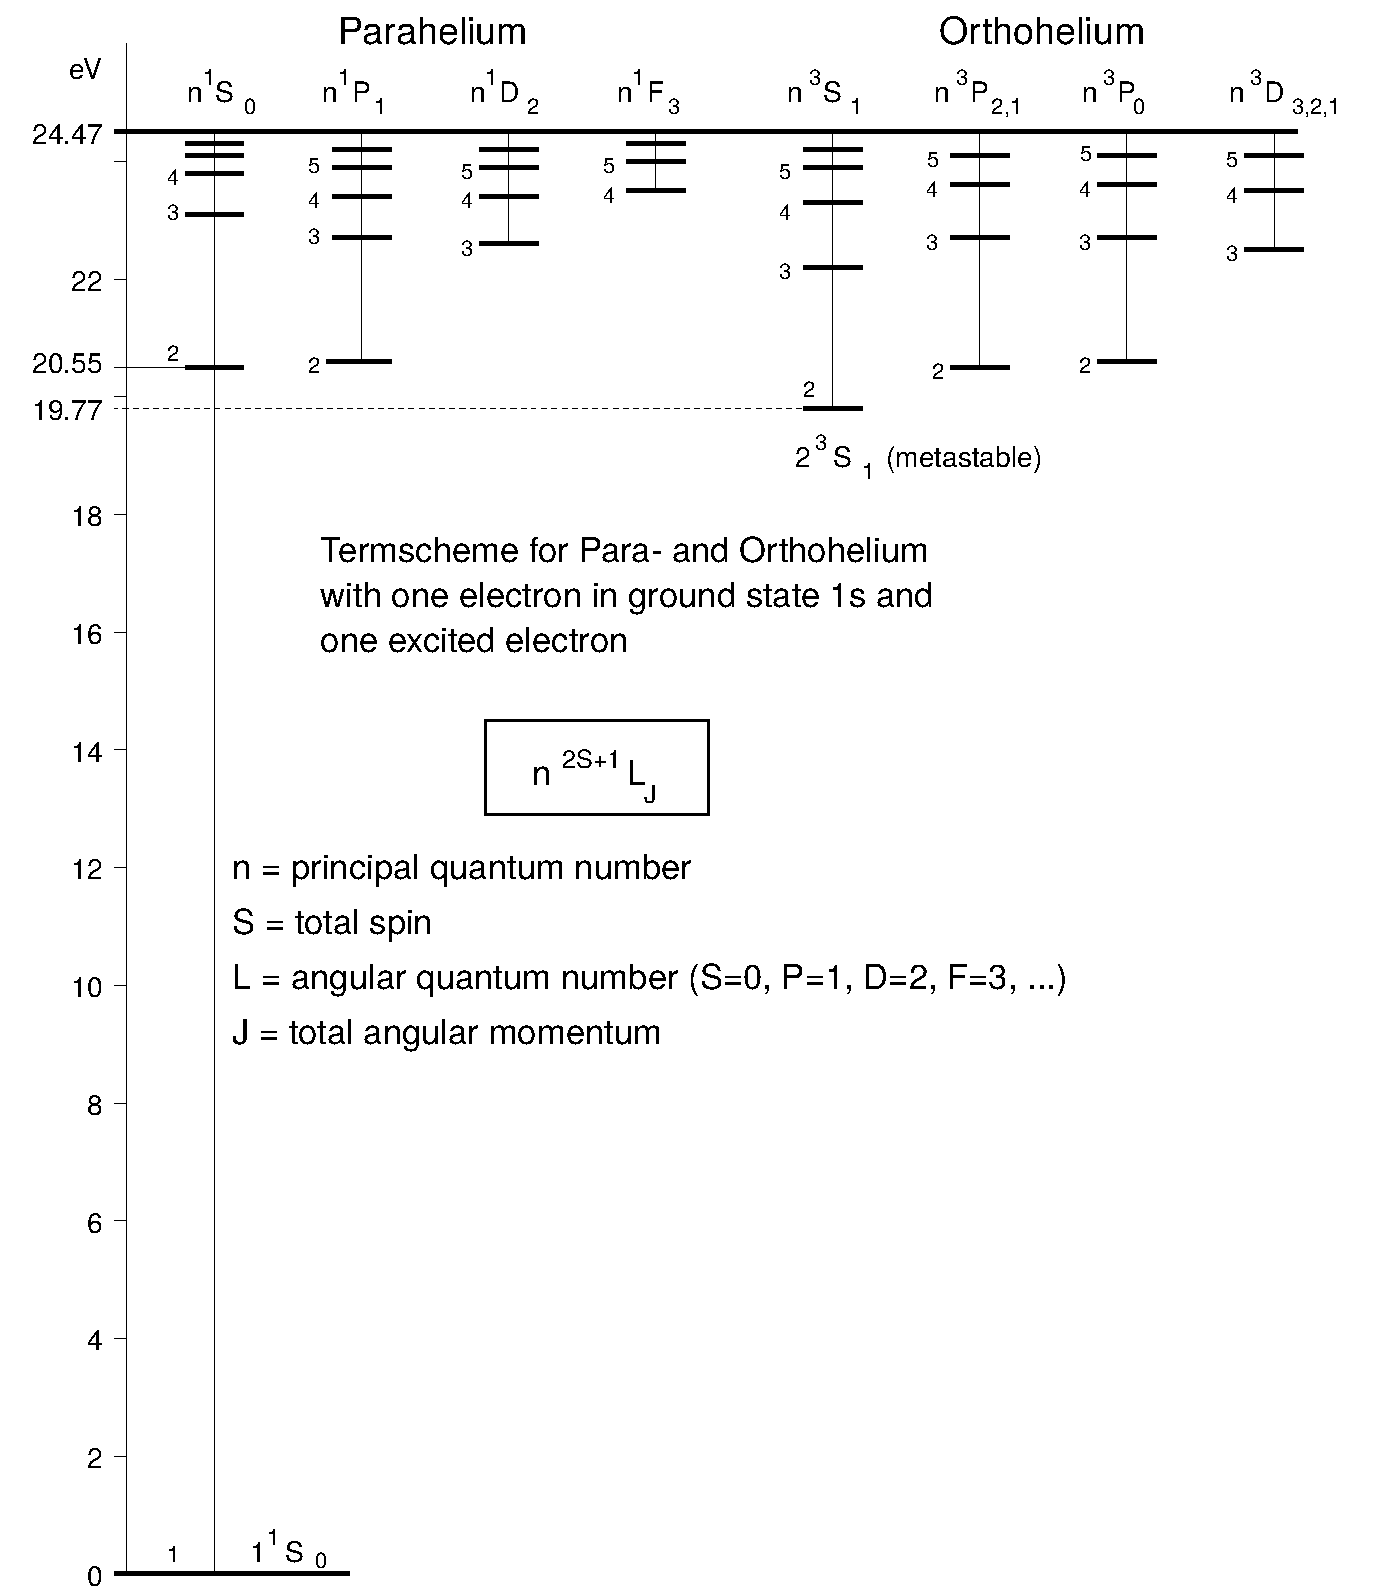
\includegraphics[width=8cm]{Helium-term-scheme.pdf}
	\caption{Termschema für Para- und Orthohelium mit einem Elektron im Grundzustand 1s und einem angeregten Elektron}
\end{figure}


\begin{align}
|1'\rangle &= |\phi_{1\uparrow}\phi_{1\downarrow}\phi_{2\uparrow}\rangle\\
|2'\rangle &= |\phi_{1\uparrow}\phi_{1\downarrow}\phi_{2\downarrow}\rangle\\
|3'\rangle &= |\phi_{1\uparrow}\phi_{1\downarrow}\phi_{3\uparrow}\rangle\\
|4'\rangle &= |\phi_{1\uparrow}\phi_{1\downarrow}\phi_{3\downarrow}\rangle\\
|5'\rangle &= |\phi_{1\uparrow}\phi_{2\uparrow}\phi_{2\downarrow}\rangle\\
|6'\rangle &= |\phi_{1\uparrow}\phi_{1\downarrow}\phi_{2\uparrow}\rangle\\
|7'\rangle &= |\phi_{2\uparrow}\phi_{2\downarrow}\phi_{3\uparrow}\rangle\\
|8'\rangle &= |\phi_{2\uparrow}\phi_{2\downarrow}\phi_{3\downarrow}\rangle\\
|9'\rangle &= |\phi_{2\uparrow}\phi_{3\uparrow}\phi_{3\downarrow}\rangle\\
|10'\rangle &= |\phi_{2\downarrow}\phi_{3\downarrow}\phi_{3\uparrow}\rangle\\
|11'\rangle &= |\phi_{1\uparrow}\phi_{3\uparrow}\phi_{3\downarrow}\rangle\\
|12'\rangle &= |\phi_{1\downarrow}\phi_{3\uparrow}\phi_{3\downarrow}\rangle\\
\end{align}





\newpage
\section{Coupled Cluster}
Molecular Electronic Structure Hamiltonian:
\begin{equation}
\hat{H}=\sum_{pq}h_{pq}\hat{a}_{p}^{\dagger}\hat{a}_{q}+\frac{1}{2}\sum_{pqrs}h_{pqrs}\hat{a}_{p}^{\dagger}\hat{a}_{q}^{\dagger}\hat{a}_{r}\hat{a}_{s}
\end{equation}
Cluster Operator:
\begin{equation}
\hat{T}=\hat{T}_1+\hat{T}_2+\hat{T}_3+\cdots\hat{T}_n
\end{equation}
with
\begin{equation}
\hat{T}_1=\sum_{i}\sum_{a}c_{a}^{i}\hat{a}_{a}^{\dagger}\hat{a}_{i}
\end{equation}
and
\begin{equation}
\hat{T}_2=\frac{1}{4}\sum_{i_1,i_2}\sum_{a_1,a_2}c_{a_1,a_2}^{i_1,i_2}\hat{a}_{a_1}^{\dagger}\hat{a}_{a_2}^{\dagger}\hat{a}_{i_1}\hat{a}_{i_2}
\end{equation}
Cluster operator that creates linear combinations of all possible $n$-tuply excited determinants:
\begin{equation}
\hat{T}_{n}=\frac{1}{(n!)^2}\sum_{i_1,i_2,...,i_n}\sum_{a_1,a_2,...,a_n}c_{a_1,a_2,...,a_n}^{i_1,i_2,...,i_n}\hat{a}_{a_1}^{\dagger}\hat{a}_{a_2}^{\dagger}\cdots\hat{a}_{a_n}^{\dagger}\hat{a}_{i_1}\hat{a}_{i_2}\cdots\hat{a}_{i_n}
\end{equation}
Electronic Schrödinger equation:
\begin{equation}
\hat{H}|\Psi\rangle = E|\Psi\rangle
\end{equation}
Coupled Cluster ansatz:
\begin{equation}
|\Psi\rangle = e^{\hat{T}}|\Psi_0\rangle
\end{equation}

In contrast to density functional theory, wavefunction-based post-Hartree-Fock methods are computationally more demanding. But they have the advantage that their accuracy can be systematically improved by using a larger basis set and including more parts of the correlation energy, although it is not straightforward to do so in a computationally efficient way. A variety of advanced wave function methods have been developed, such as configuration interaction, coupled cluster, and Möller-Plesset perturbation theory. CCSD(T) is regarded as the gold standard of electronic structure methods, which allows for a relatively cost-efficient solution of the time-independent Schrödinger equation for the ground state.

The Pauli principle requires that the total wave function must be totally antisymmetric with respect to the interchange of two electrons. Since Slater determinants have the desired symmetry properties, the wave function can be set up as a linear combination of Slater determinants. The total wave function is constructed from a so-called reference determinant $|\Phi_0\rangle$, which in turn contains optimized molecular orbitals of the form
\begin{equation}
|\phi_i\rangle=\sum_{\nu=1}^{K}|\xi_{\nu}\rangle\langle\xi_{\nu}|\phi_i\rangle
\end{equation}
whose coefficients $\langle\xi_{\nu}|\phi_i\rangle$ usually stem from a restricted Hartree Fock calculaton. From a given basis set of $K$ optimized molecular orbitals $|\phi_1\rangle,...,|\phi_K\rangle$ a total of $k=\displaystyle\binom{2K}{N}$ different $N$-electron Slater determinants can be generated. In second quantization a cluster operator can be defined, which generates linear combinations of all possible $1,2,...,n$-fold excited determinants:
\begin{equation}
\hat{T}=\hat{T}_1+\hat{T}_2+\hat{T}_3+\cdots\hat{T}_n
\end{equation}
It is explicitly written out as follows:
\begin{align}
\hat{T} =& \underbrace{\sum_{i}\sum_{a}c_{a}^{i}\hat{a}_{a}^{\dagger}\hat{a}_{i}}_{\mathrm{single}\;\mathrm{excitations}}+\underbrace{\frac{1}{4}\sum_{i_1,i_2}\sum_{a_1,a_2}c_{a_1,a_2}^{i_1,i_2}\hat{a}_{a_1}^{\dagger}\hat{a}_{a_2}^{\dagger}\hat{a}_{i_1}\hat{a}_{i_2}}_{\mathrm{double}\;\mathrm{excitations}}\\
&+\cdots + \underbrace{\frac{1}{(n!)^2}\sum_{i_1,i_2,...,i_n}\sum_{a_1,a_2,...,a_n}c_{a_1,a_2,...,a_n}^{i_1,i_2,...,i_n}\hat{a}_{a_1}^{\dagger}\hat{a}_{a_2}^{\dagger}\cdots\hat{a}_{a_n}^{\dagger}\hat{a}_{i_1}\hat{a}_{i_2}\cdots\hat{a}_{i_n}}_{n-\mathrm{fold}\;\mathrm{excitations}}
\end{align}
The conceptually simplest approach is to apply the cluster operator directly to the reference determinant:
\begin{equation}
|\Psi\rangle = \hat{T}|\Phi_0\rangle = \sum_{j=1}^{k}c_j|\Phi_j\rangle
\end{equation}
Plugging this ansatz into the Schrödinger equation \eqref{Schrödinger equation} and applying the Rayleigh-Ritz principle provides the method of full configuration interaction. However, the huge number of Slater determinants to be considered makes this method impractical. In addition, the results are not size consistent if higher excitations are neglected. One solution to the problem is to use the coupled cluster approach
\begin{equation}
|\Psi\rangle = e^{\hat{T}}|\Phi_0\rangle
\end{equation}
which applies the cluster operator in the form of an exponential. This makes it possible to explicitly include only single and double excitations and still obtain a significantly larger part of the correlation energy than with the Configuration Interaction method.


\section{DLPNO-CCSD(T)}
In contrast to density functional theory, wavefunction-based post-Hartree-Fock methods are computationally more demanding. But they have the advantage that their accuracy can be systematically improved by using a larger basis set and including more parts of the correlation energy, although it is not straightforward to do so in a computationally efficient way. A variety of advanced wave function methods have been developed, such as configuration interaction (CI), coupled cluster (CC), and Möller-Plesset perturbation theory. CCSD(T) is regarded as the gold standard of electronic structure methods, which allows for a relatively cost-efficient solution of the time-independent Schrödinger equation for the ground state.

The Pauli principle requires that the total wave function must be totally antisymmetric with respect to the interchange of two electrons. Since Slater determinants have the desired symmetry properties, the wave function can be set up as a linear combination of Slater determinants. In Coupled Cluster theory, the wave function is formally constructed as the exponential of the so called excitation operator applied to the reference determinant:
\begin{equation}
|\Psi\rangle = e^{\hat{T}}|\Psi_0\rangle\label{CC_expansion}
\end{equation}
For the CCSD method, the excitation operator $\hat{T}$ is composed of two parts
\begin{equation}
\hat{T} = \hat{T}_1 + \hat{T}_2
\end{equation}
which generate linear combinations of all possible 1- and 2-fold excited determinants. The insertion of \eqref{CC_expansion} into the electronic Schrödinger equation and projection onto the determinant states yields the CCSD equations:
\begin{align}
\langle\Psi_0|e^{-(\hat{T}_1+\hat{T}_2)}\hat{H}_{\mathrm{el}}e^{(\hat{T}_1+\hat{T}_2)}|\Psi_0\rangle &= E\\
\langle\Psi_{i}^{a}|e^{-(\hat{T}_1+\hat{T}_2)}\hat{H}_{\mathrm{el}}e^{(\hat{T}_1+\hat{T}_2)}|\Psi_0\rangle &= R_{i}^{a} = 0\\
\langle\Psi_{ij}^{ab}|e^{-(\hat{T}_1+\hat{T}_2)}\hat{H}_{\mathrm{el}}e^{(\hat{T}_1+\hat{T}_2)}|\Psi_0\rangle &= R_{ij}^{ab} = 0
\end{align}
Hierbei handelt es sich um ein Matrix-Eigenwert-Problem. Bevor die CCSD-Gleichungen gelöst werden, wird immer zuerst eine Hartree-Fock-Rechnung durchgeführt, im Falle von Singulett-Grundzuständen sind dies Restricted Hartree-Fock-Rechnungen. Die erhaltenen Molekülorbitale gehen dann als Bestandteile der Slater-Determinanten in die CCSD-Rechnungen ein.

Die exakte Lösung der CCSD-Gleichungen skaliert allerdings mit $O(N^6)$ und damit sehr unvorteilhaft mit der Systemgröße. Daher wurde die DLPNO-Methode ("Domain based local pair natural orbital") entwickelt. Diese ermöglicht es, Terme, die null ergeben, von vornherein aus der Berechnung auszuschließen. Damit kann eine nahezu lineare Skalierung erreicht werden. In der DLPNO-Methode werden nicht direkt die Hartree-Fock-Molekülorbitale verwendet. Stattdessen werden lokalisierte PAOs ("projected atomic orbitals") verwendet, für die zuerst die Molekülorbitale lokalisiert werden und dann die lokalisierten MOs $\{|i\rangle\}$ auf Atomorbitale $|\mu\rangle$ projiziert wird:
\begin{equation}
|\tilde{\mu}\rangle = \Big(1-\sum_{i}|i\rangle\langle i|\Big)|\mu\rangle
\end{equation}









\section{Complete Active Space Self Consistent Field (CASSCF)}



\section{Density Matrix Renormalization Group (DMRG)}










































\chapter{Relativistic Many-Electron Theory}


\section{Electromagnetic Field Lagrangian}

The complete Lagrangian of a classical relativistic particle coupled to the electromagnetic field is given by
\begin{equation}
	\mathcal{L} = -mc^2\sqrt{1-\frac{\vec{v}^2}{c^2}}-\frac{1}{4\mu_0}F_{\mu\nu}F^{\mu\nu}-A_{\mu}J^{\mu}
\end{equation}
Using the definitions of the four-potential and the four-current,
\begin{equation}
	J^{\mu} = (c\rho, \vec{j})\qquad\qquad\qquad A_{\mu}= (\frac{1}{c}\phi, -\vec{A})
\end{equation}
and by omitting the vacuum electromagnetic field Lagrangian, we arrive at
\begin{equation}
	\mathcal{L} = -mc^2\sqrt{1-\frac{\vec{v}^2}{c^2}}+q\vec{v}\cdot\vec{A}-q\phi
\end{equation}
Now the Euler-Lagrange equations will be used to derive the equations of motion for the classical particle in the electromagnetic field:
\begin{equation}
	\frac{\mathrm{d}}{\mathrm{d}t}\nabla_{\vec{v}}\mathcal{L}-\nabla_{\vec{x}}\mathcal{L}=0
\end{equation}











\begin{figure}[H]
	\centering
	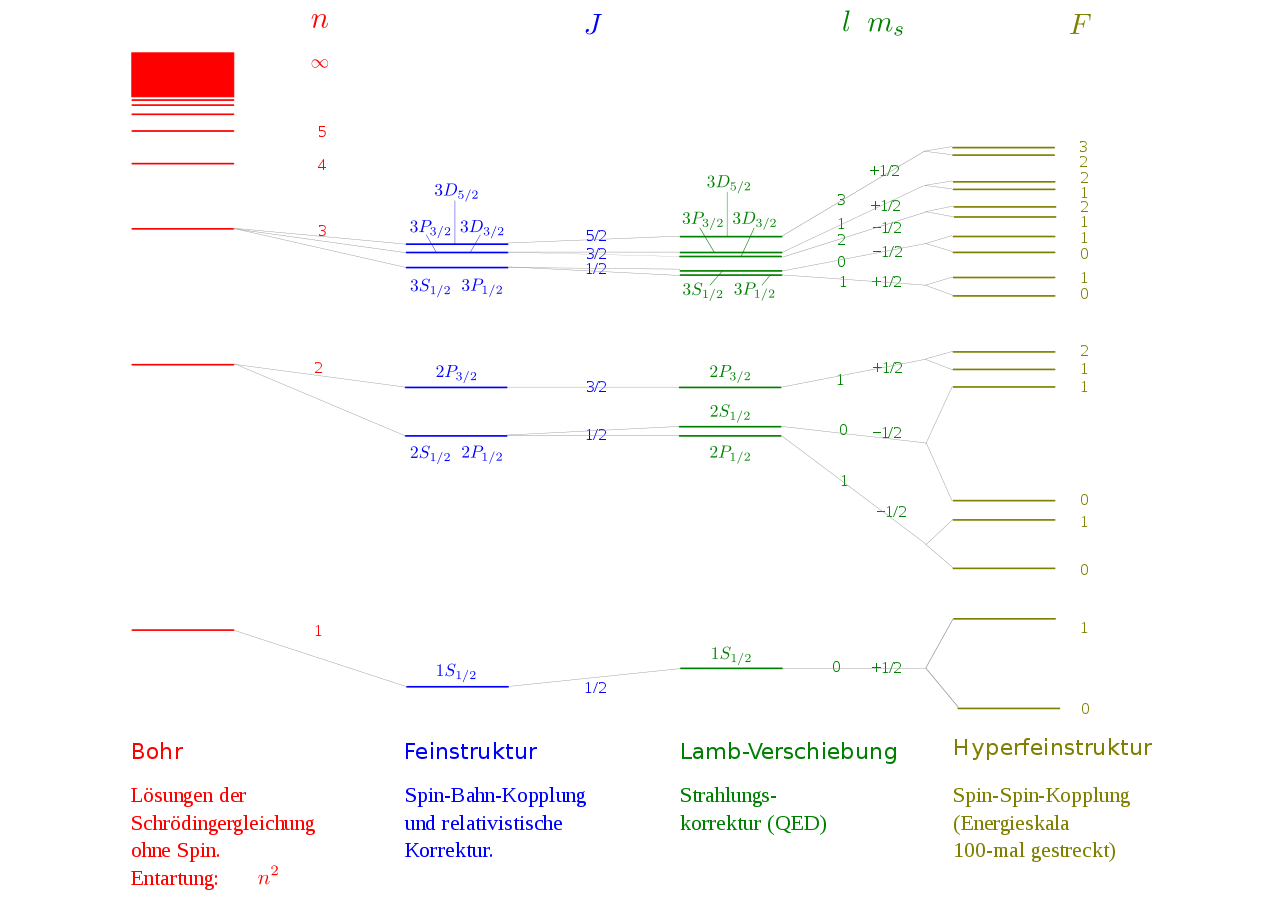
\includegraphics[width=16cm]{Wasserstoff_Aufspaltung.png}
	\caption{Termschema des Wasserstoffatoms}
\end{figure}
\url{https://de.wikipedia.org/wiki/Feinstruktur_(Physik)#/media/Datei:Wasserstoff_Aufspaltung.svg}

\newpage
\section{Dirac Equation}
The Dirac equation is a fundamental equation that describes the properties and behavior of fermions like the electron. It is a partial differential equation of first order in space and time. Thus, it is invariant under Lorentz transformation, satisfies the laws of special relativity and especially the energy momentum relation
\begin{equation}
E = \sqrt{p^2c^2+m^2c^4}
\end{equation}
Each solution of the Dirac equation for a particle corresponds to a specific state of that particle which must be described by a four component wave function called a Dirac spinor:
\begin{equation}
|\Psi\rangle := \Psi(\vec{r},t) = 
\left(\begin{array}{c} \Psi_1(\vec{r},t)  \\  \Psi_2(\vec{r},t)  \\  \Psi_3(\vec{r},t)  \\  \Psi_4(\vec{r},t)   \\\end{array}\right)
\end{equation}
This is in contrast to spin-included nonrelativistic quantum mechanics where the state of an electron is described by a two component wave function. In the Schrödinger form, the Dirac equation can be written as
\begin{equation}
\mathrm{i}\hbar\frac{\partial}{\partial t}|\Psi\rangle = \hat{H}^{\mathrm{D}}|\Psi\rangle 
\end{equation}
with the free-particle Dirac Hamiltonian
\begin{equation}
\hat{H}^{\mathrm{D}}=\boldsymbol{\beta}mc^2 +c\,\boldsymbol{\alpha}\cdot\hat{\boldsymbol{p}}
\end{equation}

\begin{equation}
\boldsymbol{\alpha}=
\left(\begin{array}{c}  
\boldsymbol{\alpha}_1
\\
\boldsymbol{\alpha}_2
\\
\boldsymbol{\alpha}_3
\end{array}\right)
\end{equation}



\begin{equation}
\hat{H}^{\mathrm{D}}=\frac{\hbar}{\mathrm{i}}c\sum_{j=1}^{3}\alpha_{j}\frac{\partial}{\partial r_j}+mc^2\beta
\end{equation}
with
\begin{equation}
\renewcommand{\arraystretch}{1.1}
\alpha_{j}=
\left(\begin{array}{cc}
0 & \sigma_j
\\
\sigma_j & 0
\\\end{array}\right)
\qquad\qquad
\beta =
\left(\begin{array}{cc}
I & 0
\\
0 & I
\\\end{array}\right)
\end{equation}
where $\sigma_j$ are the Pauli spin matrices and $I$ are 2$\times$2 identity matrices.


\section{Bethe-Salpeter Equation}








\section{Dirac-Coulomb Equation}
The Dirac-Coulomb equation can be obtained from the non-relativistic, time-dependent many-particle Schrödinger equation by exchanging the kinetic energy operator for the electrons with one-electron Dirac Hamiltonian terms. This leads to the following many-particle Hamiltonian:
\begin{equation}
\hat{H}^{\mathrm{DC}}=\underbrace{-\sum_{\alpha=1}^{K}\frac{\hbar^2}{2m_{\alpha}}\nabla_{\alpha}^2-\sum_{i=1}^{N}\hat{H}_{i}^{\mathrm{D}}}_{\hat{T}_K+\hat{T}_e}\underbrace{+\frac{1}{4\pi\epsilon_{0}}\sum_{\beta=1}^{K}\sum_{\alpha<\beta}^{K}\frac{Z_{\alpha}Z_{\beta}e^2}{\Vert\vec{R}_{\alpha}-\vec{R}_{\beta}\Vert}}_{\hat{V}_{KK}}\underbrace{+\frac{1}{4\pi\epsilon_{0}}\sum_{j=1}^{N}\sum_{i<j}^{N}\frac{e^2}{\Vert\vec{r}_{i}-\vec{r}_{j}\Vert}}_{\hat{V}_{ee}}\underbrace{-\frac{1}{4\pi\epsilon_{0}}\sum_{\alpha=1}^{K}\sum_{i=1}^{N}\frac{Z_{\alpha}e^2}{\Vert\vec{r}_{i}-\vec{R}_{\alpha}\Vert}}_{\hat{V}_{Ke}}\notag
\end{equation}







\section{Dirac-Coulomb-Breit Equation}




\section{Foldy-Wouthuysen Transformation}
\url{http://www.physik.uni-oldenburg.de/Docs/home/seminars/theo3/relQM/fwt/fwt.html}\\
\url{http://www.physik.uni-oldenburg.de/Docs/home/seminars/theo3/relQM/dirac/dirac.html}




\section{Pauli Equation and Stern-Gerlach Experiment}





\section{Breit-Pauli Equation}






\section{EPR/NMR Parameters}

\subsection{Zero Field Splitting ($\boldsymbol{D}$-Tensor)}
The Zero Field Splitting Hamiltonian is in general given by
\begin{equation}
\hat{H}_{\mathrm{ZFS}}=\hat{\vec{S}}\boldsymbol{D}\hat{\vec{S}}
\end{equation}
with the total spin operator $\hat{\vec{S}}$ of the system and the so called D-Tensor which can be written in a diagonalized form:
\begin{equation}
\boldsymbol{D}=
\end{equation}






\subsection{Electronic $\boldsymbol{g}$-Tensor}

\subsection{Hyperfine Interaction ($\boldsymbol{A}$-Tensor)}

\subsection{Nuclear $\boldsymbol{g}$-Tensor}

\subsection{Indirect Nuclear Spin-Spin Interaction}
The Diamagnetic spin-orbit term, also called $"$electron coupled nuclear spin-spin interaction$"$, is given by the Hamiltonian
\begin{equation}
\hat{H}^{\mathrm{DSO}}=\frac{e^2}{2m_e}\frac{\mu_0^2}{16\pi^2}\frac{1}{\hbar^2}\sum_{i,\nu,\nu'}g_{\nu}g_{\nu'}\mu_{\nu}\mu_{\nu'}\frac{(\hat{\vec{I}}_{\nu}\times\vec{r}_{i\nu})\cdot(\hat{\vec{I}}_{\nu'}\times\vec{r}_{i\nu'})}{r_{i\nu}^{3}r_{i\nu'}^{3}}
\end{equation}



\newpage
\section{EPR/NMR Spin Hamiltonian}
\begin{figure}[H]
	\centering
	\includegraphics[width=18cm]{chlorophyll_2.png}
	\caption{Positive and negative electron spin density of a chlorophyll a radical cation, derived from an unrestricted Kohn-Sham density functional theory calculation.}
\end{figure}
\begin{equation}
\hat{H}_{\mathrm{EPR}} = \mu_{\mathrm{B}}\vec{B}_{0}\boldsymbol{g}_{e}\hat{\vec{S}} + \hat{\vec{S}}\boldsymbol{D}\hat{\vec{S}} + \hat{\vec{S}}\boldsymbol{A}\hat{\vec{I}} - g_{n}\mu_{n}\hat{\vec{I}}\vec{B}_{0} + \hat{\vec{I}}\boldsymbol{Q}\hat{\vec{I}}
\end{equation}



\section{Quantum Electrodynamics}

\subsection{Dirac Equation in Covariant Form}
The Dirac equation in Schrödinger representation is given by
\begin{equation}
\mathrm{i}\hbar\frac{\partial}{\partial t}\psi = \hat{H}^{\mathrm{D}}\psi
\end{equation}
The relativistic Hamiltonian $\hat{H}^{\mathrm{D}}$ is given by
\begin{equation}
\hat{H}^{\mathrm{D}}=\boldsymbol{\beta}mc^2+c\boldsymbol{\alpha}\cdot\hat{\boldsymbol{p}}
\end{equation}
Now the scalar product can be multiplied out:
\begin{equation}
0=-\mathrm{i}\hbar\frac{\partial}{\partial t}\psi+\boldsymbol{\beta}mc^{2}\psi+c\alpha_{1}\hat{p}_{1}\psi +c\alpha_{2}\hat{p}_{2}\psi +c\alpha_{3}\hat{p}_{3}\psi
\end{equation}
After multiplication with the Dirac gamma matrix $\gamma^0$ and being aware of the relations
\begin{equation}
\beta=\gamma^0,\qquad\beta\gamma^0=I,\qquad I\psi=\psi,\qquad\alpha_{1}\gamma^{0}=\gamma^{1},\qquad\alpha_{2}\gamma^{0}=\gamma^{2},\qquad\alpha_{3}\gamma^{0}=\gamma^{3},
\end{equation}
we obtain
\begin{equation}
0 = \mathrm{i}\hbar\gamma^{0}\frac{1}{c}\frac{\partial}{\partial t}\psi +\mathrm{i}\hbar\gamma^{1}\frac{\partial}{\partial x_1}\psi +\mathrm{i}\hbar\gamma^{2}\frac{\partial}{\partial x_2}\psi +\mathrm{i}\hbar\gamma^{3}\frac{\partial}{\partial x_3}\psi -mc\psi
\end{equation}
This finally gives the covariant formulation of the Dirac equation:
\begin{equation}
0=\big(\mathrm{i}\hbar\gamma^{\mu}\partial_{\mu}-mc\big)\psi
\end{equation}
The corresponding definitions are
\begin{equation}
\gamma^{\mu}
=
\left(\begin{array}{c}  
\gamma^{0}
\\
\gamma^{1}
\\
\gamma^{2}
\\
\gamma^{3}
\end{array}\right),
\qquad\qquad
\partial_{\mu}
=
\left(\begin{array}{c}  
\partial_{t}/c
\\
\partial_{x_1}
\\
\partial_{x_2}
\\
\partial_{x_3}
\end{array}\right)
\end{equation}






\subsection{QED Lagrangian}
\begin{equation}
\mathcal{L}_{\mathrm{QED}}=\sum_{n}\bar{\psi}_{n}(i\gamma^{\mu}\partial_{\mu}-m_{n})\psi_{n}-\frac{1}{4}F_{\mu\nu}F^{\mu\nu}-\sum_{n}q_{n}\bar{\psi}_{n}\gamma^{\mu}A_{\mu}\psi_{n}
\end{equation}

\subsection{Electron Magnetic Dipole Moment}
\begin{equation}
\langle p_{f}|j^{\mu}|p_{i}\rangle = \bar{u}(p_{f})\bigg\{ F_{1}(q^2)\gamma^{\mu} +\frac{i\sigma^{\mu\nu}}{2m_{e}}q_{\nu}F_{2}(q^2)+i\epsilon^{\mu\nu\rho\sigma}\sigma_{\rho\sigma}q_{\nu}F_{3}(q^2) +\frac{1}{2m_e}\bigg(q^{\mu}-\frac{q^2}{2m}\gamma^{\mu}\bigg)\gamma_{5}F_{4}(q^2)\bigg\}u(p_i)
\end{equation}

\subsection{Bethe-Salpeter Equation}

\subsection{Two-Body Dirac Equations}

\subsection{Proton Spin Crisis}









































\newpage

\chapter{Density Functional Theory (DFT)}

\section{Electron Density}

\section{Hohenberg-Kohn Theorem}

\section{Kohn-Sham Equations}
In density functional theory, the ground state energy of a many-electron system is approximately determined by solving the so-called Kohn-Sham equations. The Kohn-Sham equations are based on the introduction of a fictitious reference system in which the electrons do not interact directly with each other, but only indirectly via an effective potential $V_{\mathrm{eff}}(\vec{r})$. Thus an effective one-particle operator can be introduced, the Kohn-Sham operator:
\begin{equation}
\hat{f}^{\mathrm{KS}}=-\frac{1}{2}\nabla^{2}+V_{\mathrm{eff}}(\vec{r})
\end{equation}
It is a formal analog of the Fock operator. Similar to the Hartree-Fock method, a one-electron Schrödinger equation (or Schrödinger-like equation)
\begin{equation}
\hat{f}^{\mathrm{KS}}|\phi_i\rangle = \varepsilon_{i}|\phi_i\rangle
\end{equation}
can be defined with it. The Kohn-Sham orbitals are similar to the molecular orbitals from HF calculations, but they do not have the same physically descriptive meaning. To find an expression for the effective potential $V_{\mathrm{eff}}(\vec{r})$, one starts from the general expression for the energy functional:
\begin{align}
E_{\mathrm{tot}}[\rho(\vec{r})] &= T_{\mathrm{S}}[\rho]+J[\rho]+E_{\mathrm{XC}}[\rho]+E_{\mathrm{Ne}}[\rho]\\
&= T_{\mathrm{S}}[\rho]+\frac{1}{2}\iint\frac{\rho(\vec{r}_1)\rho(\vec{r}_2)}{r_{12}}\mathrm{d}^{3}r_{1}\mathrm{d}^{3}r_2 +E_{\mathrm{XC}}[\rho] +\int V_{\mathrm{Ne}}\rho(\vec{r})\mathrm{d}^{3}r
\end{align}
The electron density for an $N$-electron system is taken as the sum of all occupied squared Kohn-Sham orbitals:
\begin{equation}
\rho(\vec{r})=\sum_{i=1}^{N}|\phi_i(\vec{r})|^2
\end{equation}
With this, a large part of the energy functional can be expressed as a functional of the Kohn-Sham orbitals:
\begin{align}
E_{\mathrm{tot}}[\{\phi_i\}] =& -\frac{1}{2}\sum_{i}^{N}\langle\phi_i|\nabla^2|\phi_i\rangle +\frac{1}{2}\sum_{i}^{N}\sum_{j}^{N}\iint|\phi_i(\vec{r}_1)|^{2}\frac{1}{r_{12}}|\phi_j(\vec{r}_2)|^{2}\mathrm{d}^{3}r_{1}\mathrm{d}^{3}r_2 + E_{\mathrm{XC}}[\rho]\\ &-\sum_{i}^{N}\int\sum_{A}^{M}\frac{Z_A}{r_{1A}}|\phi_i(\vec{r}_1)|^{2}\mathrm{d}^{3}r_1
\end{align}
Analogous to the derivation of the Hartree-Fock equations, the method of Lagrange multipliers can now be used to minimize the functional
\begin{equation}
\mathcal{L}=E_{\mathrm{tot}}[\{\phi_i\}]-\sum_{i=1}^{N}\varepsilon_i(1-\langle\phi_i|\phi_i\rangle)
\end{equation}
via
\begin{equation}
\frac{\partial\mathcal{L}}{\partial\phi_i^*}=0
\end{equation}
The result of this calculation are $N$ uncoupled one-electron eigenvalue equations of the form
\begin{equation}
\bigg(-\frac{1}{2}\nabla^2 +\underbrace{\int\frac{1}{r_{12}}\rho(\vec{r}_2)\mathrm{d}^{3}r_2+\frac{\delta E_{\mathrm{XC}}}{\delta\rho(\vec{r}_1)}-\sum_{A}^{M}\frac{Z_A}{r_{1A}}}_{=V_{\mathrm{eff}}(\vec{r})}\bigg)|\phi_i\rangle =\varepsilon_{i}|\phi_i\rangle
\end{equation}
The expression obtained for the effective potential depends explicitly on the Kohn-Sham orbitals, so that the Kohn-Sham equations have to be solved iteratively to self-consistency, just like the Hartree-Fock equations. A basis set expansion of the form
\begin{equation}
|\phi_i\rangle=\sum_{\nu=1}^{K}|\xi_{\nu}\rangle\langle\xi_{\nu}|\phi_i\rangle
\end{equation}
is used to solve the Kohn-Sham equations. Insertion into the Kohn-Sham equations and successive multiplication from the left with $\langle\xi_1|,\langle\xi_2|,...,\langle\xi_K|$ yields the matrix form of the Kohn-Sham equations:
\begin{equation}
\boldsymbol{f}^{\mathrm{KS}}\boldsymbol{c}=\varepsilon\boldsymbol{S}\boldsymbol{c}
\end{equation}
which can be diagonalized with standard methods of linear algebra.




\section{Exchange-Correlation Functionals}

\section{Density Functional Tight Binding (DFTB)}

\section{Time-Dependent Density Functional Theory (TD-DFT)}
\url{https://www.youtube.com/watch?v=ZYsktRlhMOg}










\chapter{Transition State Optimizations}

Wenn man mit einer Potentialhyperfläche $E(\vec{R})$ startet und ein Minimum auf dieser PES sucht, ist der Startpunkt die Entwicklung der PES in einer Taylorreihe:
\begin{equation}
E(\vec{R}_k +\Delta\vec{R})\approx E(\vec{R})+\nabla E(\vec{R}_k)^{\mathrm{T}}\Delta\vec{R} +\frac{1}{2}\Delta\vec{R}^{\mathrm{T}}\boldsymbol{B}\Delta\vec{R}
\end{equation}
Hier ist $\boldsymbol{B}\in\mathbb{R}^{3N\times 3N}$ die Hessematrix. Der Gradient dieser angenäherten Reihenentwicklung ist gegeben durch
\begin{equation}
\nabla E(\vec{R}_k+\Delta\vec{R})\approx \nabla E(\vec{R}_k) +\boldsymbol{B}\Delta\vec{R}
\end{equation}
Wenn dieser Gradient null gesetzt wird, ergibt sich der Newton-Schritt:
\begin{equation}
\Delta\vec{R}=-\boldsymbol{B}^{-1}\nabla E(\vec{R}_k)
\end{equation}



\section{Nudged Elastic Band Method (NEB)}



\section{BFGS Algorithm}
Vorteil: Die Hesse-Matrix muss nicht invertiert werden.

Die Quasi-Newton-Bedingung für das Update von $\boldsymbol{B}_k$ ist gegeben durch
\begin{equation}
\boldsymbol{B}_{k+1}(\vec{R}_{k+1}-\vec{R}_k) = \nabla E(\vec{R}_{k+1})-\nabla E(\vec{R}_k)
\end{equation}
Jetzt definieren wir
\begin{equation}
\vec{y}_k = \nabla E(\vec{R}_{k+1})-\nabla E(\vec{R}_k)
\end{equation}
und
\begin{equation}
\vec{s}_k = \vec{R}_{k+1} - \vec{R}_{k}
\end{equation}
Algorithm:
\begin{itemize}
	\item Obtain a direction $\Delta\vec{R}$ by calculating $-\boldsymbol{B}^{-1}\nabla E(\vec{R}_k)$
	\item Perform a line search to find an optimal stepsize $\alpha_k = \arg\min E(\vec{R}_{k}+\alpha\Delta\vec{R})$
	\item Set $\vec{s}_k = \alpha_k\Delta\vec{R}$ and $\vec{R}_{k+1}=\vec{R}_k+\vec{s}_k$
	\item Calculate $\vec{R}_k = \nabla E(\vec{R}_{k+1}) - \nabla E(\vec{R}_k)$
	\item Update Hessian matrix: $\boldsymbol{B}_{k+1}=\boldsymbol{B}_{k}+\frac{\vec{y}_k\vec{y}_k^{T}}{\vec{y}_k^{T}\vec{s}_k} - \frac{\boldsymbol{B}_k\vec{s}_k\vec{s}_k^{T}\boldsymbol{B}_k^{T}}{\vec{s}_{k}^{T}\boldsymbol{B}_k\vec{s}_k}$
\end{itemize}






\section{L-BFGS Algorithm}































\newpage

\chapter{Quantenchemische Rechnungen}

\section{Einführung in ORCA Quantum Chemistry}
\begin{itemize}
	\item ChemSpider aufrufen und ein Molekül auswählen. Auf den \textit{Save}-Button drücken, um ein *.mol-File des Moleküls abzuspeichern.
	\item Die *.mol-Datei in einem neu angelegten Ordner in der Orca-Direction ablegen
	\item Ein neues Terminal öffnen und in den Ordner wechseln
	\item Das Programm OpenBabel mit dem Befehl \textit{openbabel.obgui} öffnen
	\item Unter \textit{Input Format} den Dateityp \textit{mol -- MDL MOL format} auswählen
	\item Mit dem ...-Button die jeweilige *.mol-Datei aufrufen
	\item Die Einstellungsmöglichkeiten \textit{Add hydrogens (make explicit)} und \textit{Generate 3D coordinates} bestätigen
	\item Unter \textit{Output Format} den Dateityp \textit{xyz -- XYZ cartesian coordinates format} auswählen
	\item Auf den ...-Button klicken und eine *.xyz-Datei erzeugen
	\item Durch Betätigen des \textit{Convert}-Buttons bestätigen
	\item Das Programm OpenBabel beenden
	\item gedit aus dem Dateiordner aufrufen und ein Orca-Inputfile erzeugen
	\item Vergewissern, dass man sich im Terminal im Ordner befindet, in dem Inputfile und xyz-File liegen
	\item Dann den folgenden Befehl in das Terminal eingeben, um Orca zu aktivieren: \begin{verbatim}
	echo 'export PATH=$HOME/orca:$PATH' >> ~/.bash_profile; source ~/.bash_profile
	\end{verbatim}
	\item Rechnung starten über (Beispiel):
	\begin{verbatim}
	orca Dateiname.inp > output.out
	\end{verbatim}
	\item Einen durch das Programm molekel lesbaren Dateityp mit folgendem Befehl erzeugen: \begin{verbatim}
	orca_2mkl Dateiname -molden
	\end{verbatim}
	\item In den Ordner wechseln, in dem molekel liegt und das Programm mit folgendem Befehl öffnen:
	\begin{verbatim}
	david@david-Aspire-V3-372:~/molekel_5_4_0_linux_x86_64$ ./launch_molekel.sh
	\end{verbatim}
\end{itemize}

\section{Mit ZMatrix-Editor}
Um ein Molekül zu berechnen, wird folgendermaßen vorgegangen:
\begin{itemize}
	\item molden aus dem jeweiligen Verzeichnis starten, in dem Inputdateien und xyz-Files liegen sollen.
	\item Im \textit{Molden Control}-Fenster die Schaltfläche \textit{ZMAT Editor} auswählen. Man gelangt ins \textit{Zmatrix Editor}-Fenster.
	\item \textit{Substitute atom by fragment} und dann das richtige Fragment auswählen.
	\item Im \textit{MOLDEN}-Fenster ein Atom auswählen, an das ein weiteres Fragment angefügt werden soll und dies erneut auswählen.
	\item So fortfahren bis Konstruktion des Moleküls abgeschlossen ist.
	\item Ins \textit{Zmatrix Editor}-Fenster wechseln und unter Format \textit{Cartesian} $\to$ \textit{XYZ} auswählen
	\item File name mit xyz-Endung eingeben und mit \textit{Write Z-Matrix} bestätigen.
	\item molden verlassen und mit einem Texteditor eine Input-Datei erzeugen.
	\item Rechnung starten über (Beispiel): orca butan.inp > output.out
\end{itemize}





\section{Eigenes Hartree-Fock-Programm}
\url{http://nznano.blogspot.com/2018/03/simple-quantum-chemistry-hartree-fock.html}

























\chapter{Trash}

\section{Calculation of NMR/EPR Properties}

\subsection{Nuclear Spin}
The elementary components of which protons and neutrons are composed of are called \textbf{quarks}.




Die elementaren Bestandteile, aus denen Protonen und Neutronen bestehen, werden \textbf{Quarks} genannt. Der Drehimpuls $\hat{\vec{S}}$ eines Quark erfüllt die folgenden gekoppelten Eigenwertgleichungen:
\begin{align}
\hat{\vec{S}}^{\;2}\big|s,s_{z}\big\rangle &= \hbar^{2}s(s+1)\big|s,s_{z}\big\rangle\\
\hat{S}_{z}\big|s,s_{z}\big\rangle &= \hbar s_{z}\big|s,s_{z}\big\rangle
\end{align}
Quarks haben die Spinquantenzahl $s=\frac{1}{2}$ und sind somit Fermionen. Die Flavour-Quantenzahl $I_{z}$ wird als Isospin bezeichnet. Sie beschreibt eine innere Symmetrie unter der starken Wechselwirkung. Sogenannte up-Quarks haben einen Isospin von $s_{z}=+\frac{1}{2}$, down-Quarks einen Isospin von $s_{z}=-\frac{1}{2}$. Ein Proton besteht aus zwei up-Quarks und einem down-Quark (uud), ein Neutron aus einem up-Quark und zwei down-Quarks (udd). Die Spins mehrerer Protonen und Neutronen in einem Atomkern koppeln gemäß den Regeln der Quantenmechanik zu einem Gesamtdrehimpuls, der als \textbf{Kernspin} $\vec{I}$ bezeichnet wird:
\begin{equation}
\vec{I}=\sum_{i=1}^{A}\vec{S}_{i}
\end{equation}
Dabei ist $A$ die Gesamtzahl aller Quarks im Atomkern. Da die Quantenzahl $s_z$ die Ausrichtung eines Spins $\vec{S}$ und damit die Quantenzahl $s$ bestimmt (siehe Clebsch-Gordon-Koeffizienten), ergibt sich der Gesamtspin eines Kerns
\begin{equation}
|\vec{I}|=\sqrt{I(I+1)}\hbar
\end{equation}
zu null, falls die Anzahl von Neutronen und Protonen im Kern übereinstimmt. Atomkerne mit einer ungleichen Zahl von Neutronen und Protonen besitzen ein \textbf{magnetisches Moment}
\begin{equation}
\vec{\mu}_{I}=\gamma\vec{I}=\frac{g_{I}\mu_{\mathrm{K}}}{\hbar}\vec{I},
\end{equation}
wobei $\gamma$ das gyromagnetische Verhältnis, $g_{I}$ der Kern-$g$-Faktor und $\mu_{\mathrm{K}}$ das Kern-Magneton ist. 





\subsection{Effective NMR Spin-Hamiltonian}
The full NMR Hamiltonian of an arbitrary organic molecule consisting of $N$ hydrogen protons is given by
\begin{equation}
\hat{H}_{\mathrm{z}} = \gamma B_0\sum_{i=1}^{N}(1-\sigma_i)\hat{I}_{iz} +2\pi\sum_{i=1}^{N-1}\sum_{j=i+1}^{N}J_{ij}\hat{\vec{I}}_{i}\hat{\vec{I}}_{j}\label{Zeeman effect}
\end{equation}
where $\gamma$ is the gyromagnetic ratio, $B_0$ is the static magnetic field in $z$-direction applied to the probe and $\sigma_i$ is the chemical shift experienced by the $i$-th proton in the molecule. For the $z$-component $\hat{I}_{iz}$ of the $i$-th spin operator a representation in a specific basis is needed. For this purpose it is common to chose the uncoupled $"$product basis$"$ which is simply given by tensor products of the wavefunctions $|s,m\rangle_i =|m_i\rangle$ for individual proton spins:
\begin{equation}
|n\rangle = |m_1\rangle\otimes|m_2\rangle\otimes\cdots\otimes|m_N\rangle = \bigotimes_{i=1}^{N}|m_i\rangle
\end{equation}
Note that the basis states in the corresponding dual space are given by
\begin{equation}
\langle n| = \langle m_N|\otimes\langle m_{N-1}|\otimes\cdots\otimes\langle n_1|
\end{equation}
The basis states can be used to define the identity operator
\begin{equation}
\hat{\mathbbm{1}}=\sum_{n}|n\rangle\langle n|
\end{equation}
Now we can expand the Zeeman Hamiltonian \eqref{Zeeman effect} in terms of these spin states:
\begin{align}
\hat{H}_{\mathrm{z}} &= \gamma B_0\sum_{i=1}^{N}\hat{\mathbbm{1}}(1-\sigma_i)\hat{I}_{iz}\hat{\mathbbm{1}} = \gamma B_0\sum_{i=1}^{N}\sum_{n}|n\rangle\langle n|(1-\sigma_i)\hat{I}_{iz}\sum_{n'}|n'\rangle\langle n'|\\
&= \gamma B_0\sum_{i=1}^{N}(1-\sigma_i)\sum_{n,n'}\langle n|\hat{I}_{iz}|n'\rangle|n\rangle\langle n'|
\end{align}
As an example we take 







Zuerst sollen die Eigenfunktionen von $\hat{\vec{S}}^{\,2}$ bzw. $\hat{S}_{z}$ durch Übergang in die Matrixschreibweise ermittelt werden. Auch für den Spin sind die Matrixelemente durch \eqref{Eigenwertergebnis 1} und \eqref{Eigenwertergebnis 2} festgelegt:
\begin{align}
\big\langle s,s_{z}'\big|\hat{\vec{S}}^{\;2}\big|s,s_{z}\big\rangle &= \hbar^{2}s(s+1)\delta_{s_{z}s_{z}'}
\\
\big\langle s,s_{z}'\big|\hat{S}_{z}\big|s,s_{z}\big\rangle &= \hbar \,s_{z}\,\delta_{s_{z}s_{z}'}
\\
\big\langle s,s_{z}'\big|\hat{S}_{+}\big|s,s_{z}\big\rangle &= \hbar\sqrt{(s-s_{z})(s+s_{z}+1)}\,\delta_{s_{z}'s_{z}+1}
\\
\big\langle s,s_{z}'\big|\hat{S}_{-}\big|s,s_{z}\big\rangle &= \hbar\sqrt{(s+s_{z})(s-s_{z}+1)}\,\delta_{s_{z}'s_{z}-1}
\end{align}
Die obigen Operatoren werden in der $\{\big|\uparrow\big\rangle,\big|\downarrow\big\rangle\}$-Basis durch $2\times 2$-Matrizen dargestellt:
\begin{equation}
\renewcommand{\arraystretch}{1.4}
\hat{S}_{i}:=
\left(\begin{array}{cc}
\big\langle \uparrow\big|\hat{S}_i\big|\uparrow\big\rangle
&
\big\langle \uparrow\big|\hat{S}_i\big|\downarrow\big\rangle
\\
\big\langle \downarrow\big|\hat{S}_i\big|\uparrow\big\rangle
& 
\big\langle \downarrow\big|\hat{S}_i\big|\downarrow\big\rangle
\\\end{array}\right)
\end{equation}


\url{http://easyspin.org/easyspin/documentation/hamiltonian.html}\\
\url{http://easyspin.org/easyspin/documentation/}\\
\url{https://physics.stackexchange.com/questions/244462/coupled-and-decoupled-matrix-representations-of-spin-spin-interactions}








\subsection{Spin-Orbit Coupling (SOC)}
It is very important for phosphorescence dynamics, EPR relaxation rates and Jahn-Teller effect.






















\chapter{Appendix}

\section{Ferromagnetism and Antiferromagnetism}
Electron Spin and behavior of the wavefunction under symmetry transformations (Lie Algebras). Spin Polarization. Connection between angular momentum and the magnetic moment of the electron. Ferromagnetic and Antiferromagnetic molecular aggregates. Hubbard model and Heisenberg model. Superexchange. Spin waves (magnons).



\section{Point Group Symmetry Adapted Linear Combinations (SALCs)}
\begin{itemize}
	\item MO-Schemata von Wasser, Methan und Komplexverbindungen mit Hilfe von Punktgruppen ermitteln
	\item Configuration State Functions und ihren Zusammenhang zur Elektronenkonfiguration, Drehimpulszustand und Punktgruppen verstehen
	\item Hartree-Fock-Rechnungen und erweiterte Hückel-Rechnungen von verschiedenen Molekülen mit Orca durchführen und auf Elektronenkonfiguration (z.B. Entartung von MOs) überprüfen
	\item Atomare und molekulare Termsymbole verstehen
	\item \url{https://chemistry.stackexchange.com/questions/16305/how-can-i-find-the-symmetry-labels-of-atomic-orbitals-in-a-molecule}
	\item \url{https://chem.libretexts.org/Bookshelves/Physical_and_Theoretical_Chemistry_Textbook_Maps/Book%3A_Symmetry_(Vallance)/10%3A_Matrix_Representations_of_Groups}
	\item \url{https://chemistry.stackexchange.com/questions/58229/what-do-these-labels-for-molecular-electronic-states-mean/58345#58345}
	\item \url{https://chem.libretexts.org/Bookshelves/Physical_and_Theoretical_Chemistry_Textbook_Maps/Supplemental_Modules_(Physical_and_Theoretical_Chemistry)/Quantum_Mechanics/10%3A_Multi-electron_Atoms/Quantum_Numbers_for_Atoms}
	\item 
	\url{https://chemistry.stackexchange.com/questions/16623/how-do-quantum-software-packages-work}
\end{itemize}

\subsubsection{Ethylen-Molekül}
Im Folgenden sollen symmetrieadaptierte Linearkombinationen für das Ethylen-Molekül aufgestellt werden. Das Transformationsverhalten der Basisfunktionen des minimalen Basissatzes STO-3G unter der zugehörigen Punktgruppe $D_{2h}$ ist in der nachfolgenden Tabelle beschrieben:
\begin{table}[H]
	\textbf{\caption{Transformationsverhalten}}
	\begin{center}
		\renewcommand{\arraystretch}{1.5}
		\begin{tabular}{c|cccccccccccccc}
			$D_{2h}$ &  p$_{1x}$  &  p$_{1y}$  &  p$_{1z}$  &  p$_{2x}$  &  p$_{2y}$  &  p$_{2z}$  &  1s$_{C1}$  &  2s$_{C1}$  &  1s$_{C2}$  &  2s$_{C2}$  &  s$_{H1}$  &  s$_{H2}$  &  s$_{H3}$  &  s$_{H4}$
			\\ \hline
			$E$  &  p$_{1x}$  &  p$_{1y}$  &  p$_{1z}$  &  p$_{2x}$  &  p$_{2y}$  &  p$_{2z}$  &  1s$_{C1}$  &  2s$_{C1}$  &  1s$_{C2}$  &  2s$_{C2}$  &  s$_{H1}$  &  s$_{H2}$  &  s$_{H3}$  &  s$_{H4}$
			\\  
			$C_2(x)$  &  p$_{1x}$  &  -p$_{1y}$  &  -p$_{1z}$  &  p$_{2x}$  &  -p$_{2y}$  &  -p$_{2z}$  &  1s$_{C1}$  &  2s$_{C1}$  &  1s$_{C2}$  &  2s$_{C2}$  &  s$_{H2}$  &  s$_{H1}$  &  s$_{H4}$  &  s$_{H3}$
			\\
			$C_2(y)$  &     &  
			\\
			$C_2(z)$   &    &  
			\\
			$i$   &     &   \\
			$\sigma(xy)$   &   &
			\\
			$\sigma(xz)$   &    &
			\\
			$\sigma(yz)$   &    &
		\end{tabular}
	\end{center}
\end{table}


\begin{table}[H]
	\textbf{\caption{Charaktertafel $D_{2h}$-Punktgruppe}}
	\begin{center}
		\renewcommand{\arraystretch}{1.1}
		\begin{tabular}{c|cccccccc}
			$D_{2h}$ &  $E$  &  $C_{2}(x)$  &  $C_{2}(y)$  &  $C_{2}(z)$  &  $i$  &  $\sigma(xy)$  &  $\sigma(xz)$  &  $\sigma(yz)$
			\\ \hline
			$A_g$  &  1  &  1  &  1  &  1  &  1  &  1  &  1  &  1
			\\  
			$B_{1g}$  &  1  &  -1  &  -1  &  1  &  1  &  1  &  -1  &  -1
			\\
			$B_{2g}$  &  1  &  -1  &  1  &  -1  &  1  &  -1  &  1  &  -1
			\\
			$B_{3g}$  &  1  &  1  &  -1  &  -1  &  1  &  -1  &  -1  &  1
			\\
			$A_u$  &  1  &  1  &  1  &  1  &  -1  &  -1  &  -1  &  -1
			\\
			$B_{1u}$  &  1  &  -1  &  -1  &  1  &  -1  &  -1  &  1  &  1
			\\
			$B_{2u}$  &  1  &  -1  &  1  &  -1  &  -1  &  1  &  -1  &  1
			\\
			$B_{3u}$  &  1  &  1  &  -1  &  -1  &  -1  &  1  &  1  &  -1
		\end{tabular}
	\end{center}
\end{table}


\scriptsize
\begin{equation}
E
\renewcommand{\arraystretch}{1.4}
\left(\begin{array}{c} p_{1x}  \\  p_{1y}  \\  p_{1z}  \\  p_{2x}  \\ p_{2y} \\  p_{2z}  \\  1s_{C1}  \\  2s_{C1}  \\  1s_{C2}  \\  2s_{C2}  \\  s_{H1}  \\  s_{H2}  \\  s_{H3}  \\  s_{H4}   \\\end{array}\right)
=
\left(\begin{array}{cccccccccccccc}
1 & 0 & 0 & 0 & 0 & 0 & 0 & 0 & 0 & 0 & 0 & 0 & 0 & 0
\\
0 & 1 & 0 & 0 & 0 & 0 & 0 & 0 & 0 & 0 & 0 & 0 & 0 & 0
\\
0 & 0 & 1 & 0 & 0 & 0 & 0 & 0 & 0 & 0 & 0 & 0 & 0 & 0
\\
0 & 0 & 0 & 1 & 0 & 0 & 0 & 0 & 0 & 0 & 0 & 0 & 0 & 0
\\
0 & 0 & 0 & 0 & 1 & 0 & 0 & 0 & 0 & 0 & 0 & 0 & 0 & 0
\\
0 & 0 & 0 & 0 & 0 & 1 & 0 & 0 & 0 & 0 & 0 & 0 & 0 & 0
\\
0 & 0 & 0 & 0 & 0 & 0 & 1 & 0 & 0 & 0 & 0 & 0 & 0 & 0
\\
0 & 0 & 0 & 0 & 0 & 0 & 0 & 1 & 0 & 0 & 0 & 0 & 0 & 0
\\
0 & 0 & 0 & 0 & 0 & 0 & 0 & 0 & 1 & 0 & 0 & 0 & 0 & 0
\\
0 & 0 & 0 & 0 & 0 & 0 & 0 & 0 & 0 & 1 & 0 & 0 & 0 & 0
\\
0 & 0 & 0 & 0 & 0 & 0 & 0 & 0 & 0 & 0 & 1 & 0 & 0 & 0
\\
0 & 0 & 0 & 0 & 0 & 0 & 0 & 0 & 0 & 0 & 0 & 1 & 0 & 0
\\
0 & 0 & 0 & 0 & 0 & 0 & 0 & 0 & 0 & 0 & 0 & 0 & 1 & 0
\\
0 & 0 & 0 & 0 & 0 & 0 & 0 & 0 & 0 & 0 & 0 & 0 & 0 & 1
\\\end{array}\right)
\left(\begin{array}{c} p_{1x}  \\  p_{1y}  \\  p_{1z}  \\  p_{2x}  \\ p_{2y} \\  p_{2z}  \\  1s_{C1}  \\  2s_{C1}  \\  1s_{C2}  \\  2s_{C2}  \\  s_{H1}  \\  s_{H2}  \\  s_{H3}  \\  s_{H4}   \\\end{array}\right)
\end{equation}
\normalsize




\scriptsize
\begin{equation}
C_{2}(x)
\renewcommand{\arraystretch}{1.4}
\left(\begin{array}{c} p_{1x}  \\  p_{1y}  \\  p_{1z}  \\  p_{2x}  \\ p_{2y} \\  p_{2z}  \\  1s_{C1}  \\  2s_{C1}  \\  1s_{C2}  \\  2s_{C2}  \\  s_{H1}  \\  s_{H2}  \\  s_{H3}  \\  s_{H4}   \\\end{array}\right)
=
\left(\begin{array}{cccccccccccccc}
1 & 0 & 0 & 0 & 0 & 0 & 0 & 0 & 0 & 0 & 0 & 0 & 0 & 0
\\
0 & -1 & 0 & 0 & 0 & 0 & 0 & 0 & 0 & 0 & 0 & 0 & 0 & 0
\\
0 & 0 & -1 & 0 & 0 & 0 & 0 & 0 & 0 & 0 & 0 & 0 & 0 & 0
\\
0 & 0 & 0 & 1 & 0 & 0 & 0 & 0 & 0 & 0 & 0 & 0 & 0 & 0
\\
0 & 0 & 0 & 0 & -1 & 0 & 0 & 0 & 0 & 0 & 0 & 0 & 0 & 0
\\
0 & 0 & 0 & 0 & 0 & -1 & 0 & 0 & 0 & 0 & 0 & 0 & 0 & 0
\\
0 & 0 & 0 & 0 & 0 & 0 & 1 & 0 & 0 & 0 & 0 & 0 & 0 & 0
\\
0 & 0 & 0 & 0 & 0 & 0 & 0 & 1 & 0 & 0 & 0 & 0 & 0 & 0
\\
0 & 0 & 0 & 0 & 0 & 0 & 0 & 0 & 1 & 0 & 0 & 0 & 0 & 0
\\
0 & 0 & 0 & 0 & 0 & 0 & 0 & 0 & 0 & 1 & 0 & 0 & 0 & 0
\\
0 & 0 & 0 & 0 & 0 & 0 & 0 & 0 & 0 & 0 & 0 & 1 & 0 & 0
\\
0 & 0 & 0 & 0 & 0 & 0 & 0 & 0 & 0 & 0 & 1 & 0 & 0 & 0
\\
0 & 0 & 0 & 0 & 0 & 0 & 0 & 0 & 0 & 0 & 0 & 0 & 0 & 1
\\
0 & 0 & 0 & 0 & 0 & 0 & 0 & 0 & 0 & 0 & 0 & 0 & 1 & 0
\\\end{array}\right)
\left(\begin{array}{c} p_{1x}  \\  p_{1y}  \\  p_{1z}  \\  p_{2x}  \\ p_{2y} \\  p_{2z}  \\  1s_{C1}  \\  2s_{C1}  \\  1s_{C2}  \\  2s_{C2}  \\  s_{H1}  \\  s_{H2}  \\  s_{H3}  \\  s_{H4}   \\\end{array}\right)
\end{equation}
\normalsize



\scriptsize
\begin{equation}
C_{2}(y)
\renewcommand{\arraystretch}{1.4}
\left(\begin{array}{c} p_{1x}  \\  p_{1y}  \\  p_{1z}  \\  p_{2x}  \\ p_{2y} \\  p_{2z}  \\  1s_{C1}  \\  2s_{C1}  \\  1s_{C2}  \\  2s_{C2}  \\  s_{H1}  \\  s_{H2}  \\  s_{H3}  \\  s_{H4}   \\\end{array}\right)
=
\left(\begin{array}{cccccccccccccc}
0 & 0 & 0 & -1 & 0 & 0 & 0 & 0 & 0 & 0 & 0 & 0 & 0 & 0
\\
0 & 0 & 0 & 0 & 1 & 0 & 0 & 0 & 0 & 0 & 0 & 0 & 0 & 0
\\
0 & 0 & 0 & 0 & 0 & -1 & 0 & 0 & 0 & 0 & 0 & 0 & 0 & 0
\\
-1 & 0 & 0 & 0 & 0 & 0 & 0 & 0 & 0 & 0 & 0 & 0 & 0 & 0
\\
0 & 1 & 0 & 0 & 0 & 0 & 0 & 0 & 0 & 0 & 0 & 0 & 0 & 0
\\
0 & 0 & -1 & 0 & 0 & 0 & 0 & 0 & 0 & 0 & 0 & 0 & 0 & 0
\\
0 & 0 & 0 & 0 & 0 & 0 & 0 & 0 & 1 & 0 & 0 & 0 & 0 & 0
\\
0 & 0 & 0 & 0 & 0 & 0 & 0 & 0 & 0 & 1 & 0 & 0 & 0 & 0
\\
0 & 0 & 0 & 0 & 0 & 0 & 1 & 0 & 0 & 0 & 0 & 0 & 0 & 0
\\
0 & 0 & 0 & 0 & 0 & 0 & 0 & 1 & 0 & 0 & 0 & 0 & 0 & 0
\\
0 & 0 & 0 & 0 & 0 & 0 & 0 & 0 & 0 & 0 & 0 & 0 & 0 & 1
\\
0 & 0 & 0 & 0 & 0 & 0 & 0 & 0 & 0 & 0 & 0 & 0 & 1 & 0
\\
0 & 0 & 0 & 0 & 0 & 0 & 0 & 0 & 0 & 0 & 0 & 1 & 0 & 0
\\
0 & 0 & 0 & 0 & 0 & 0 & 0 & 0 & 0 & 0 & 1 & 0 & 0 & 0
\\\end{array}\right)
\left(\begin{array}{c} p_{1x}  \\  p_{1y}  \\  p_{1z}  \\  p_{2x}  \\ p_{2y} \\  p_{2z}  \\  1s_{C1}  \\  2s_{C1}  \\  1s_{C2}  \\  2s_{C2}  \\  s_{H1}  \\  s_{H2}  \\  s_{H3}  \\  s_{H4}   \\\end{array}\right)
\end{equation}
\normalsize


\scriptsize
\begin{equation}
C_{2}(z)
\renewcommand{\arraystretch}{1.4}
\left(\begin{array}{c} p_{1x}  \\  p_{1y}  \\  p_{1z}  \\  p_{2x}  \\ p_{2y} \\  p_{2z}  \\  1s_{C1}  \\  2s_{C1}  \\  1s_{C2}  \\  2s_{C2}  \\  s_{H1}  \\  s_{H2}  \\  s_{H3}  \\  s_{H4}   \\\end{array}\right)
=
\left(\begin{array}{cccccccccccccc}
0 & 0 & 0 & -1 & 0 & 0 & 0 & 0 & 0 & 0 & 0 & 0 & 0 & 0
\\
0 & 0 & 0 & 0 & -1 & 0 & 0 & 0 & 0 & 0 & 0 & 0 & 0 & 0
\\
0 & 0 & 0 & 0 & 0 & 1 & 0 & 0 & 0 & 0 & 0 & 0 & 0 & 0
\\
-1 & 0 & 0 & 0 & 0 & 0 & 0 & 0 & 0 & 0 & 0 & 0 & 0 & 0
\\
0 & -1 & 0 & 0 & 0 & 0 & 0 & 0 & 0 & 0 & 0 & 0 & 0 & 0
\\
0 & 0 & 1 & 0 & 0 & 0 & 0 & 0 & 0 & 0 & 0 & 0 & 0 & 0
\\
0 & 0 & 0 & 0 & 0 & 0 & 0 & 0 & 1 & 0 & 0 & 0 & 0 & 0
\\
0 & 0 & 0 & 0 & 0 & 0 & 0 & 0 & 0 & 1 & 0 & 0 & 0 & 0
\\
0 & 0 & 0 & 0 & 0 & 0 & 1 & 0 & 0 & 0 & 0 & 0 & 0 & 0
\\
0 & 0 & 0 & 0 & 0 & 0 & 0 & 1 & 0 & 0 & 0 & 0 & 0 & 0
\\
0 & 0 & 0 & 0 & 0 & 0 & 0 & 0 & 0 & 0 & 0 & 0 & 1 & 0
\\
0 & 0 & 0 & 0 & 0 & 0 & 0 & 0 & 0 & 0 & 0 & 0 & 0 & 1
\\
0 & 0 & 0 & 0 & 0 & 0 & 0 & 0 & 0 & 0 & 1 & 0 & 0 & 0
\\
0 & 0 & 0 & 0 & 0 & 0 & 0 & 0 & 0 & 0 & 0 & 1 & 0 & 0
\\\end{array}\right)
\left(\begin{array}{c} p_{1x}  \\  p_{1y}  \\  p_{1z}  \\  p_{2x}  \\ p_{2y} \\  p_{2z}  \\  1s_{C1}  \\  2s_{C1}  \\  1s_{C2}  \\  2s_{C2}  \\  s_{H1}  \\  s_{H2}  \\  s_{H3}  \\  s_{H4}   \\\end{array}\right)
\end{equation}
\normalsize


\scriptsize
\begin{equation}
i
\renewcommand{\arraystretch}{1.4}
\left(\begin{array}{c} p_{1x}  \\  p_{1y}  \\  p_{1z}  \\  p_{2x}  \\ p_{2y} \\  p_{2z}  \\  1s_{C1}  \\  2s_{C1}  \\  1s_{C2}  \\  2s_{C2}  \\  s_{H1}  \\  s_{H2}  \\  s_{H3}  \\  s_{H4}   \\\end{array}\right)
=
\left(\begin{array}{cccccccccccccc}
0 & 0 & 0 & -1 & 0 & 0 & 0 & 0 & 0 & 0 & 0 & 0 & 0 & 0
\\
0 & 0 & 0 & 0 & 1 & 0 & 0 & 0 & 0 & 0 & 0 & 0 & 0 & 0
\\
0 & 0 & 0 & 0 & 0 & 1 & 0 & 0 & 0 & 0 & 0 & 0 & 0 & 0
\\
-1 & 0 & 0 & 0 & 0 & 0 & 0 & 0 & 0 & 0 & 0 & 0 & 0 & 0
\\
0 & 1 & 0 & 0 & 0 & 0 & 0 & 0 & 0 & 0 & 0 & 0 & 0 & 0
\\
0 & 0 & 1 & 0 & 0 & 0 & 0 & 0 & 0 & 0 & 0 & 0 & 0 & 0
\\
0 & 0 & 0 & 0 & 0 & 0 & 0 & 0 & 1 & 0 & 0 & 0 & 0 & 0
\\
0 & 0 & 0 & 0 & 0 & 0 & 0 & 0 & 0 & 1 & 0 & 0 & 0 & 0
\\
0 & 0 & 0 & 0 & 0 & 0 & 1 & 0 & 0 & 0 & 0 & 0 & 0 & 0
\\
0 & 0 & 0 & 0 & 0 & 0 & 0 & 1 & 0 & 0 & 0 & 0 & 0 & 0
\\
0 & 0 & 0 & 0 & 0 & 0 & 0 & 0 & 0 & 0 & 0 & 0 & 0 & 1
\\
0 & 0 & 0 & 0 & 0 & 0 & 0 & 0 & 0 & 0 & 0 & 0 & 1 & 0
\\
0 & 0 & 0 & 0 & 0 & 0 & 0 & 0 & 0 & 0 & 0 & 1 & 0 & 0
\\
0 & 0 & 0 & 0 & 0 & 0 & 0 & 0 & 0 & 0 & 1 & 0 & 0 & 0
\\\end{array}\right)
\left(\begin{array}{c} p_{1x}  \\  p_{1y}  \\  p_{1z}  \\  p_{2x}  \\ p_{2y} \\  p_{2z}  \\  1s_{C1}  \\  2s_{C1}  \\  1s_{C2}  \\  2s_{C2}  \\  s_{H1}  \\  s_{H2}  \\  s_{H3}  \\  s_{H4}   \\\end{array}\right)
\end{equation}
\normalsize



\scriptsize
\begin{equation}
\sigma(xy)
\renewcommand{\arraystretch}{1.4}
\left(\begin{array}{c} p_{1x}  \\  p_{1y}  \\  p_{1z}  \\  p_{2x}  \\ p_{2y} \\  p_{2z}  \\  1s_{C1}  \\  2s_{C1}  \\  1s_{C2}  \\  2s_{C2}  \\  s_{H1}  \\  s_{H2}  \\  s_{H3}  \\  s_{H4}   \\\end{array}\right)
=
\left(\begin{array}{cccccccccccccc}
1 & 0 & 0 & 0 & 0 & 0 & 0 & 0 & 0 & 0 & 0 & 0 & 0 & 0
\\
0 & 1 & 0 & 0 & 0 & 0 & 0 & 0 & 0 & 0 & 0 & 0 & 0 & 0
\\
0 & 0 & -1 & 0 & 0 & 0 & 0 & 0 & 0 & 0 & 0 & 0 & 0 & 0
\\
0 & 0 & 0 & 1 & 0 & 0 & 0 & 0 & 0 & 0 & 0 & 0 & 0 & 0
\\
0 & 0 & 0 & 0 & 1 & 0 & 0 & 0 & 0 & 0 & 0 & 0 & 0 & 0
\\
0 & 0 & 0 & 0 & 0 & -1 & 0 & 0 & 0 & 0 & 0 & 0 & 0 & 0
\\
0 & 0 & 0 & 0 & 0 & 0 & 1 & 0 & 0 & 0 & 0 & 0 & 0 & 0
\\
0 & 0 & 0 & 0 & 0 & 0 & 0 & 1 & 0 & 0 & 0 & 0 & 0 & 0
\\
0 & 0 & 0 & 0 & 0 & 0 & 0 & 0 & 1 & 0 & 0 & 0 & 0 & 0
\\
0 & 0 & 0 & 0 & 0 & 0 & 0 & 0 & 0 & 1 & 0 & 0 & 0 & 0
\\
0 & 0 & 0 & 0 & 0 & 0 & 0 & 0 & 0 & 0 & 1 & 0 & 0 & 0
\\
0 & 0 & 0 & 0 & 0 & 0 & 0 & 0 & 0 & 0 & 0 & 1 & 0 & 0
\\
0 & 0 & 0 & 0 & 0 & 0 & 0 & 0 & 0 & 0 & 0 & 0 & 1 & 0
\\
0 & 0 & 0 & 0 & 0 & 0 & 0 & 0 & 0 & 0 & 0 & 0 & 0 & 1
\\\end{array}\right)
\left(\begin{array}{c} p_{1x}  \\  p_{1y}  \\  p_{1z}  \\  p_{2x}  \\ p_{2y} \\  p_{2z}  \\  1s_{C1}  \\  2s_{C1}  \\  1s_{C2}  \\  2s_{C2}  \\  s_{H1}  \\  s_{H2}  \\  s_{H3}  \\  s_{H4}   \\\end{array}\right)
\end{equation}
\normalsize



\scriptsize
\begin{equation}
\sigma(xz)
\renewcommand{\arraystretch}{1.4}
\left(\begin{array}{c} p_{1x}  \\  p_{1y}  \\  p_{1z}  \\  p_{2x}  \\ p_{2y} \\  p_{2z}  \\  1s_{C1}  \\  2s_{C1}  \\  1s_{C2}  \\  2s_{C2}  \\  s_{H1}  \\  s_{H2}  \\  s_{H3}  \\  s_{H4}   \\\end{array}\right)
=
\left(\begin{array}{cccccccccccccc}
1 & 0 & 0 & 0 & 0 & 0 & 0 & 0 & 0 & 0 & 0 & 0 & 0 & 0
\\
0 & -1 & 0 & 0 & 0 & 0 & 0 & 0 & 0 & 0 & 0 & 0 & 0 & 0
\\
0 & 0 & 1 & 0 & 0 & 0 & 0 & 0 & 0 & 0 & 0 & 0 & 0 & 0
\\
0 & 0 & 0 & 1 & 0 & 0 & 0 & 0 & 0 & 0 & 0 & 0 & 0 & 0
\\
0 & 0 & 0 & 0 & -1 & 0 & 0 & 0 & 0 & 0 & 0 & 0 & 0 & 0
\\
0 & 0 & 0 & 0 & 0 & -1 & 0 & 0 & 0 & 0 & 0 & 0 & 0 & 0
\\
0 & 0 & 0 & 0 & 0 & 0 & 1 & 0 & 0 & 0 & 0 & 0 & 0 & 0
\\
0 & 0 & 0 & 0 & 0 & 0 & 0 & 1 & 0 & 0 & 0 & 0 & 0 & 0
\\
0 & 0 & 0 & 0 & 0 & 0 & 0 & 0 & 1 & 0 & 0 & 0 & 0 & 0
\\
0 & 0 & 0 & 0 & 0 & 0 & 0 & 0 & 0 & 1 & 0 & 0 & 0 & 0
\\
0 & 0 & 0 & 0 & 0 & 0 & 0 & 0 & 0 & 0 & 0 & 1 & 0 & 0
\\
0 & 0 & 0 & 0 & 0 & 0 & 0 & 0 & 0 & 0 & 1 & 0 & 0 & 0
\\
0 & 0 & 0 & 0 & 0 & 0 & 0 & 0 & 0 & 0 & 0 & 0 & 0 & 1
\\
0 & 0 & 0 & 0 & 0 & 0 & 0 & 0 & 0 & 0 & 0 & 0 & 1 & 0
\\\end{array}\right)
\left(\begin{array}{c} p_{1x}  \\  p_{1y}  \\  p_{1z}  \\  p_{2x}  \\ p_{2y} \\  p_{2z}  \\  1s_{C1}  \\  2s_{C1}  \\  1s_{C2}  \\  2s_{C2}  \\  s_{H1}  \\  s_{H2}  \\  s_{H3}  \\  s_{H4}   \\\end{array}\right)
\end{equation}
\normalsize




\scriptsize
\begin{equation}
\sigma(yz)
\renewcommand{\arraystretch}{1.4}
\left(\begin{array}{c} p_{1x}  \\  p_{1y}  \\  p_{1z}  \\  p_{2x}  \\ p_{2y} \\  p_{2z}  \\  1s_{C1}  \\  2s_{C1}  \\  1s_{C2}  \\  2s_{C2}  \\  s_{H1}  \\  s_{H2}  \\  s_{H3}  \\  s_{H4}   \\\end{array}\right)
=
\left(\begin{array}{cccccccccccccc}
0 & 0 & 0 & -1 & 0 & 0 & 0 & 0 & 0 & 0 & 0 & 0 & 0 & 0
\\
0 & 0 & 0 & 0 & 1 & 0 & 0 & 0 & 0 & 0 & 0 & 0 & 0 & 0
\\
0 & 0 & 0 & 0 & 0 & 1 & 0 & 0 & 0 & 0 & 0 & 0 & 0 & 0
\\
-1 & 0 & 0 & 0 & 0 & 0 & 0 & 0 & 0 & 0 & 0 & 0 & 0 & 0
\\
0 & 1 & 0 & 0 & 0 & 0 & 0 & 0 & 0 & 0 & 0 & 0 & 0 & 0
\\
0 & 0 & 1 & 0 & 0 & 0 & 0 & 0 & 0 & 0 & 0 & 0 & 0 & 0
\\
0 & 0 & 0 & 0 & 0 & 0 & 0 & 0 & 1 & 0 & 0 & 0 & 0 & 0
\\
0 & 0 & 0 & 0 & 0 & 0 & 0 & 0 & 0 & 1 & 0 & 0 & 0 & 0
\\
0 & 0 & 0 & 0 & 0 & 0 & 1 & 0 & 0 & 0 & 0 & 0 & 0 & 0
\\
0 & 0 & 0 & 0 & 0 & 0 & 0 & 1 & 0 & 0 & 0 & 0 & 0 & 0
\\
0 & 0 & 0 & 0 & 0 & 0 & 0 & 0 & 0 & 0 & 0 & 0 & 0 & 1
\\
0 & 0 & 0 & 0 & 0 & 0 & 0 & 0 & 0 & 0 & 0 & 0 & 1 & 0
\\
0 & 0 & 0 & 0 & 0 & 0 & 0 & 0 & 0 & 0 & 0 & 1 & 0 & 0
\\
0 & 0 & 0 & 0 & 0 & 0 & 0 & 0 & 0 & 0 & 1 & 0 & 0 & 0
\\\end{array}\right)
\left(\begin{array}{c} p_{1x}  \\  p_{1y}  \\  p_{1z}  \\  p_{2x}  \\ p_{2y} \\  p_{2z}  \\  1s_{C1}  \\  2s_{C1}  \\  1s_{C2}  \\  2s_{C2}  \\  s_{H1}  \\  s_{H2}  \\  s_{H3}  \\  s_{H4}   \\\end{array}\right)
\end{equation}
\normalsize
Man hat somit eine reduzible Darstellung der Punktgruppe gefunden, bestehend aus acht Darstellungsmatrizen. Indem man für jede Darstellungsmatrix eine Ähnlichkeitstransformation
\begin{equation}
\boldsymbol{B} = \boldsymbol{S}^{-1}\boldsymbol{A}\boldsymbol{S}
\end{equation}
durchführt, können die Matrizen auf Blockdiagonalform gebracht werden. Die unterschiedlichen Blöcke sind die Darstellungsmatrizen der irreduziblen Darstellungen der Punktgruppe. In der Regel treten die irreduziblen Darstellungen in einer reduziblen Darstellung unterschiedlich häufig auf. Mit Hilfe der Reduktionsformel
\begin{equation}
n_{\Gamma_i}=\frac{1}{h}\sum_{R}\chi_{\Gamma_i}(R)\chi_{\Gamma_{\mathrm{red}}}(R)
\end{equation}
kann ermittelt werden, in welche irreduziblen Darstellungen die reduzible Darstellung zerfällt. Laut ORCA-Programmpaket ergibt sich für Ethylen folgende direkte Summe von Irreps:
\begin{equation}
\Gamma_{\mathrm{red}}= 4 A_{g} \oplus 2 B_{1g} \oplus B_{2g} \oplus B_{1u} \oplus 2 B_{2u} \oplus 4 B_{3u}
\end{equation}
Wendet man die Projektionsoperator-Methode auf das Ethylen-Molekül an, ergeben sich die folgenden SALCs:
\begin{table}[H]
	\textbf{\caption{SALCs des Ethylen-Moleküls}}
	\begin{center}
		\renewcommand{\arraystretch}{1.5}
		\begin{tabular}{c|cccccccccccccc}
			&  $|\varphi_1\rangle(a_g)$  &  $|\varphi_2\rangle(a_g)$  &  $|\varphi_3\rangle(b_{1g})$  &  $|\varphi_4\rangle(b_{1g})$  &  $|\varphi_4\rangle(b_{2g})$  &  $|\varphi_4\rangle(b_{2g})$  &  $|\varphi_4\rangle(b_{1u})$  &  $|\varphi_4\rangle(b_{2u})$  &  $|\varphi_4\rangle(b_{3u})$
			\\ \hline
			p$_{1x}$  &  $+0.70711$  &  $-0.70711$  &  $+0.00000$  &  $+0.00000$  &  $+0.00000$  &  $+0.00000$  &  $+0.00000$  &  $+0.00000$  &  $+0.70711$
			\\  
			p$_{1y}$  &  $+0.00000$  &  $+0.00000$  &  $+0.70711$  &  $-0.70711$  &  $+0.00000$  &  $+0.00000$  &  $+0.00000$  &  $+0.70711$  &  $+0.00000$
			\\
			p$_{1z}$  &  $+0.00000$  &  $+0.00000$  &  $+0.00000$  &  $+0.00000$  &  $+0.70711$  &  $-0.70711$  &  $+0.70711$  &  $+0.00000$  &  $+0.00000$
			\\
			p$_{2x}$  &  $-0.70711$  &  $+0.70711$  &  $+0.00000$  &  $+0.00000$  &  $+0.00000$  &  $+0.00000$  &  $+0.00000$  &  $+0.00000$  &  $+0.70711$
			\\
			p$_{2y}$  &  $+0.00000$  &  $+0.00000$  &  $-0.70711$  &  $+0.70711$  &  $+0.00000$  &  $+0.00000$  &  $+0.00000$  &  $+0.70711$  &  $+0.00000$
			\\
			p$_{2z}$  &  $+0.00000$  &  $+0.00000$  &  $+0.00000$  &  $+0.00000$  &  $-0.70711$  &  $+0.70711$  &  $+0.70711$  &  $+0.00000$  &  $+0.00000$
			\\
			1s$_{C1}$ &  $+0.00000$  &  $+0.00000$  &  $+0.00000$  &  $+0.00000$  &  $+0.00000$  &  $+0.00000$  &  $+0.00000$  &  $+0.00000$  &  $+0.00000$
			\\
			2s$_{C1}$ &  $+0.00000$  &  $+0.00000$  &  $+0.00000$  &  $+0.00000$  &  $+0.00000$  &  $+0.00000$  &  $+0.00000$  &  $+0.00000$  &  $+0.00000$
			\\
			1s$_{C2}$ &  $+0.00000$  &  $+0.00000$  &  $+0.00000$  &  $+0.00000$  &  $+0.00000$  &  $+0.00000$  &  $+0.00000$  &  $+0.00000$  &  $+0.00000$
			\\
			2s$_{C2}$ &  $+0.00000$  &  $+0.00000$  &  $+0.00000$  &  $+0.00000$  &  $+0.00000$  &  $+0.00000$  &  $+0.00000$  &  $+0.00000$  &  $+0.00000$
			\\
			s$_{H1}$  &  $+0.00000$  &  $+0.00000$  &  $+0.00000$  &  $+0.00000$  &  $+0.00000$  &  $+0.00000$  &  $+0.00000$  &  $+0.00000$  &  $+0.00000$
			\\
			s$_{H2}$  &  $+0.00000$  &  $+0.00000$  &  $+0.00000$  &  $+0.00000$  &  $+0.00000$  &  $+0.00000$  &  $+0.00000$  &  $+0.00000$  &  $+0.00000$
			\\
			s$_{H3}$  &  $+0.00000$  &  $+0.00000$  &  $+0.00000$  &  $+0.00000$  &  $+0.00000$  &  $+0.00000$  &  $+0.00000$  &  $+0.00000$  &  $+0.00000$
			\\
			s$_{H4}$  &  $+0.00000$  &  $+0.00000$  &  $+0.00000$  &  $+0.00000$  &  $+0.00000$  &  $+0.00000$  &  $+0.00000$  &  $+0.00000$  &  $+0.00000$
		\end{tabular}
	\end{center}
\end{table}
Eine Hartree-Fock-Rechnung mit den SALCs als Basisfunktionen liefert Molekülorbitale, die sich nach den irreduziblen Darstellungen der Punktgruppe $D_{2h}$ transformieren:
\begin{table}[H]
	\textbf{\caption{Symmetrieadaptierte Molekülorbitale des Ethylens}}
	\begin{center}
		\renewcommand{\arraystretch}{1.5}
		\begin{tabular}{c|cccccccccccccc}
			MO  &  Besetzung  &  Irrep
			\\ \hline
			1  &  2.00  &  $1A_{g}$
			\\  
			2  &  2.00  &  $1B_{3u}$
			\\
			3  &  2.00  &  $2A_{g}$
			\\
			4  &  2.00  &  $2B_{3u}$
			\\
			5  &  2.00  &  $1B_{2u}$
			\\
			6  &  2.00  &  $3A_{g}$
			\\
			7 &  2.00  &   $1B_{1g}$
			\\
			8 &  2.00  &   $1B_{1u}$
			\\
			9 &  0.00  &   $1B_{2g}$
			\\
			10 &  0.00  &  $2B_{2u}$
			\\
			11  &  0.00  & $4A_{g}$
			\\
			12  &  0.00  & $3B_{3u}$
			\\
			13  &  0.00  & $2B_{1g}$
			\\
			14  &  0.00  & $4B_{3u}$
		\end{tabular}
	\end{center}
\end{table}
Da jedes Molekülorbital zwei Spinorbitale liefert, ist die dominierende Grundzustands-Elektronenkonfiguration gegeben durch
\begin{equation}
(1a_{g})^2(1b_{3u})^2(2a_{g})^2(2b_{3u})^2(1b_{2u})^2(3a_{g})^2(1b_{1g})^2(1b_{1u})^2\label{Ethylen-Elektronenkonfiguration}
\end{equation}
Den Grundzustandsterm erhält man, indem man zuerst das Tensorprodukt (Kroneckerprodukt)
\begin{equation}
\underbrace{A_{g}\otimes A_{g}}_{(1a_{g})^2}\otimes\underbrace{B_{3u}\otimes B_{3u}}_{(1b_{3u})^2}\otimes \underbrace{A_{g}\otimes A_{g}}_{(2a_{g})^2}\otimes\underbrace{B_{3u}\otimes B_{3u}}_{(2b_{3u})^2}\otimes \underbrace{B_{2u}\otimes B_{2u}}_{(1b_{2u})^2}\otimes \underbrace{A_{g}\otimes A_{g}}_{(3a_{g})^2}\otimes \underbrace{B_{1g}\otimes B_{1g}}_{(1b_{1g})^2}\otimes \underbrace{B_{1u}\otimes B_{1u}}_{(1b_{1u})^2}=\Gamma_{\mathrm{red}}
\end{equation}
aller irreduziblen Darstellungen bildet, nach denen sich die Spinorbitale transformieren. Die daraus resultierende Darstellungsmatrix ist in der Regel reduzibel. Mit Hilfe der Beziehung
\begin{equation}
n_{\Gamma_i}=\frac{1}{h}\sum_{R}\chi_{\Gamma_i}(R)\chi_{\Gamma_{\mathrm{red}}}(R)\label{Reduktionsformel}
\end{equation}
kann dann ermittelt werden, wie häufig die $i$-te irreduzible Darstellung $\Gamma_i$ in der reduziblen Darstellung $\Gamma_{\mathrm{red}}$ vorkommt. Dabei macht man sich den Satz zunutze, dass der Charakter einer Produktdarstellung
\begin{equation}
\Gamma_{\mathrm{red}}=\bigotimes_{i=1}^{N}\Gamma_i
\end{equation}
gleich dem Produkt der Charaktere aller $\Gamma_i$ ist:
\begin{equation}
\chi_{\Gamma_{\mathrm{red}}}(R)=\prod_{i=1}^{N}\chi_{\Gamma_i}(R)
\end{equation}
Im Fall des Ethylens sind alle Irreps eindimensional, sodass auch in der Produktdarstellung nur eine irreduzible Darstellung enthalten sein kann. Die Berechnung nach \eqref{Reduktionsformel} zeigt, welche Irrep das ist:
\begin{align}
d......
\end{align}
Damit ergibt sich, dass die Elektronenkonfiguration \eqref{Ethylen-Elektronenkonfiguration} nur einen Term liefert, der einem Singulett-Grundzustandsterm $^{1}A_{1g}$ entspricht.










\subsubsection{Hexamminchrom(III)-Komplex}
Wir gehen im Folgenden davon aus, dass mit Hilfe eines symmetrieadaptierten Basissatzes aus SALCs eine Hartree-Fock-Rechnung des Übergangsmetallkomplexes $[\mathrm{Cr(NH_3)_6}]^{3+}$ durchgeführt wurde. Je nachdem, ob die Zentralion-Liganden-Bindungen eher ionischen oder eher kovalenten Charakter haben, haben die an der HOMO-LUMO-Grenze liegenden $e_g$- und $t_{2g}$-Molekülorbitale mehr oder weniger starken d-Orbitalcharakter.
\begin{itemize}
	\item Mögliche Terme für verschiedene d-Elektronenkonfigurationen bestimmen
	\item Configuration State Functions für diese Terme für den Fall d$^2$ und d$^3$ bestimmen
\end{itemize}
Der betrachtete Komplex hat eine oktaedrische Symmetrie und gehört daher zur Punktgruppe $O_h$. Es gibt vier mögliche Elektronenkonfigurationen, wenn man nur die d-Molekülorbitale in Form eines CAS betrachtet:
\begin{align}
& (t_{2g})^3 \\
& (t_{2g})^2(e_g)^1 \\
& (t_{2g})^1(e_g)^2 \\
& (e_g)^3
\end{align}
Mit Hilfe von \eqref{Reduktionsformel} lassen sich die irreduziblen Bestandteile zum Tensorprodukt jeder Elektronenkonfiguration bestimmen. Es ergibt sich:
\begin{align}
T_{2g}\otimes T_{2g}\otimes T_{2g} &= A_{1g}\oplus A_{2g}\oplus 2E_{g}\oplus 3T_{1g}\oplus 4T_{2g}\\
\big(T_{2g}\otimes T_{2g}\otimes E_{g} &= A_{1g}\oplus A_{2g}\oplus 2E_{g}\oplus 2T_{1g}\oplus 2T_{2g}\big)\\
T_{2g}\otimes E_{g}\otimes E_{g} &= 2T_{1g}\oplus 2T_{2g}\\
E_{g}\otimes E_{g}\otimes E_{g} &= A_{1g}\oplus A_{2g}\oplus 2E_{g}
\end{align}








Bezieht man jetzt noch die zwei $\sigma$-Molekülorbitale zweier NH$_3$-Liganden, die sich nach der irreduziblen Darstellung $E_g$ transformieren, mit in den CAS ein, werden bereits deutlich mehr Elektronenkonfigurationen möglich:









\subsubsection{CASSCF-Berechnungen}
\begin{itemize}
	\item Ergebnisse der Ethylen-Berechnung aufbereiten
	\item Sauerstoff berechnen
	\item Mg-Porphyrin berechnen
	\item Carotinoide berechnen
\end{itemize}




\subsubsection{Elektronische Struktur von Übergangsmetallkomplexen}
\begin{itemize}
	\item Jahn-Teller-Effekt
	\item Vibronische Kopplungen
	\item Spin-Bahn-Kopplung
	\item Zero Field Splitting
	\item Hyperfeinkopplung
\end{itemize}









\section{Benzene Molecular Orbitals in Hückel Approximation}

\newpage
\begin{figure}[H]
	\centering
	\begin{subfigure}[b]{0.23\textwidth}  
		\centering 
		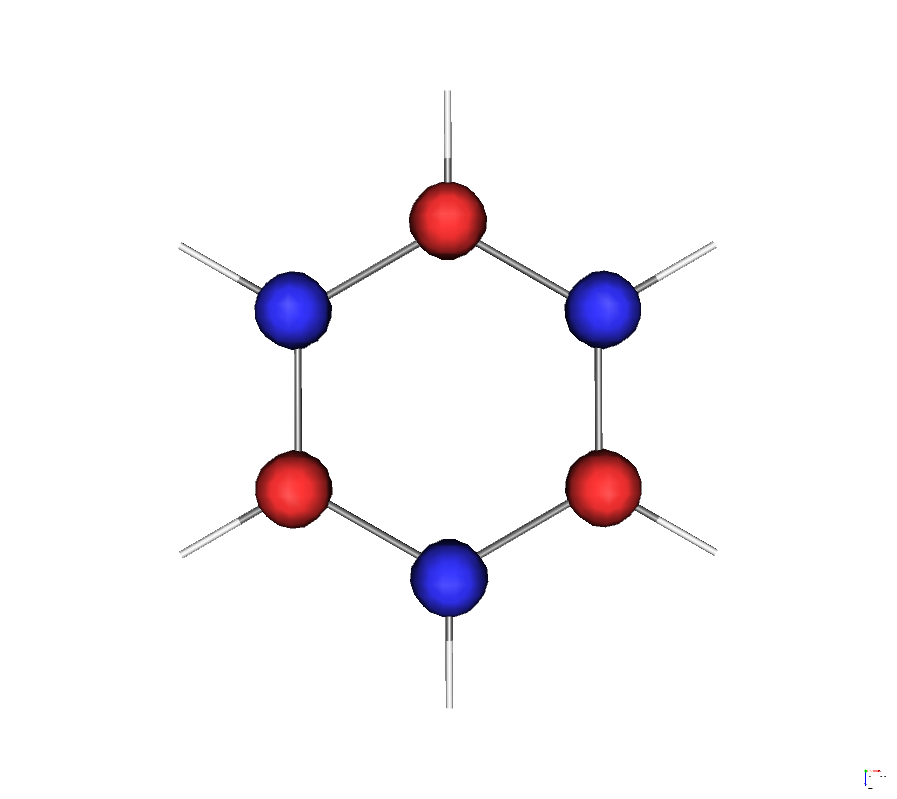
\includegraphics[width=\textwidth]{Benzol-1.png}
		\caption[]{{\small $E_1=-323.1875\,\mathrm{eV}$}}    
	\end{subfigure}
	\hfill
	\begin{subfigure}[b]{0.23\textwidth}
		\centering
		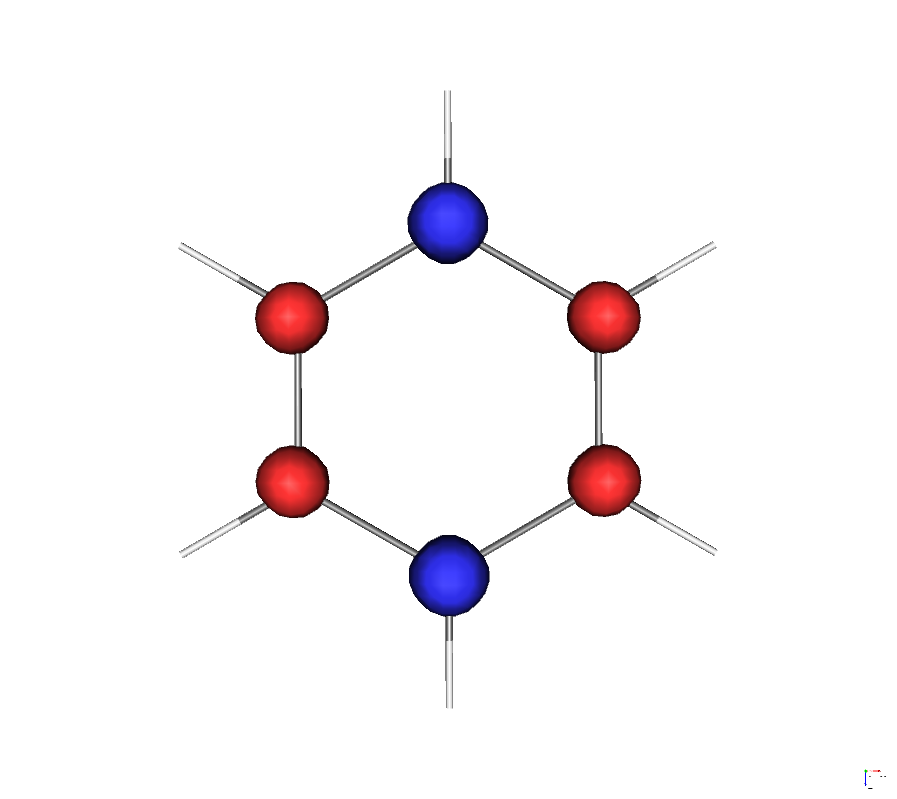
\includegraphics[width=\textwidth]{Benzol-2.png}
		\caption[Network2]{{\small $E_2=-320.2855\,\mathrm{eV}$}}
	\end{subfigure}
	\hfill
	\begin{subfigure}[b]{0.23\textwidth}
		\centering
		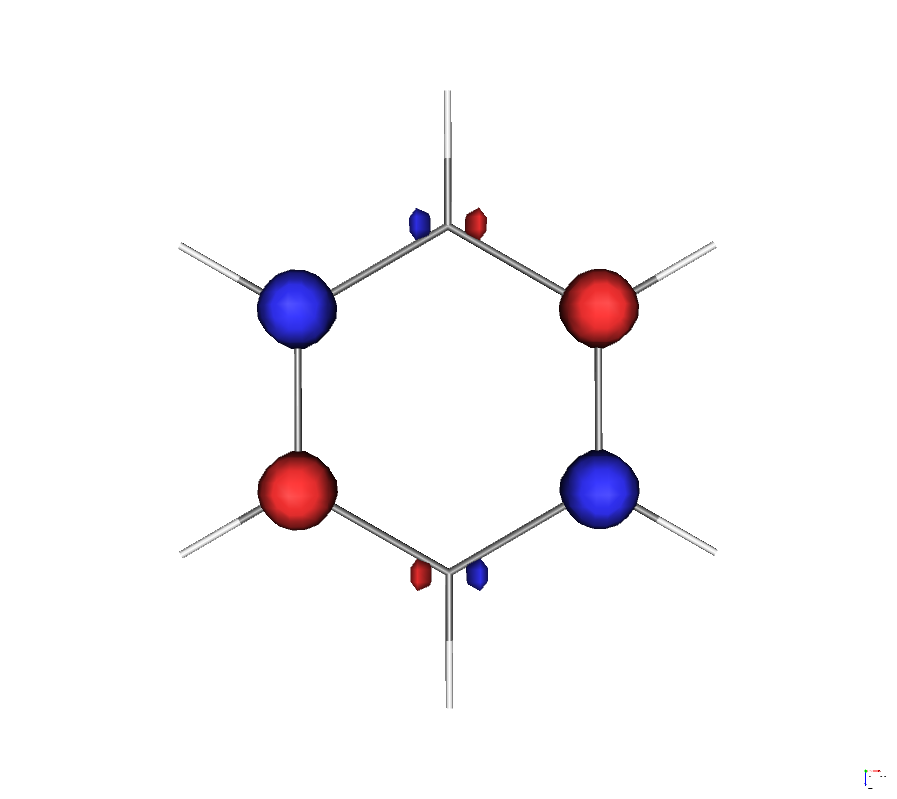
\includegraphics[width=\textwidth]{Benzol-3.png}
		\caption[Network2]{{\small $E_3=-320.2855\,\mathrm{eV}$}}
	\end{subfigure}
	\hfill
	\begin{subfigure}[b]{0.23\textwidth}
		\centering
		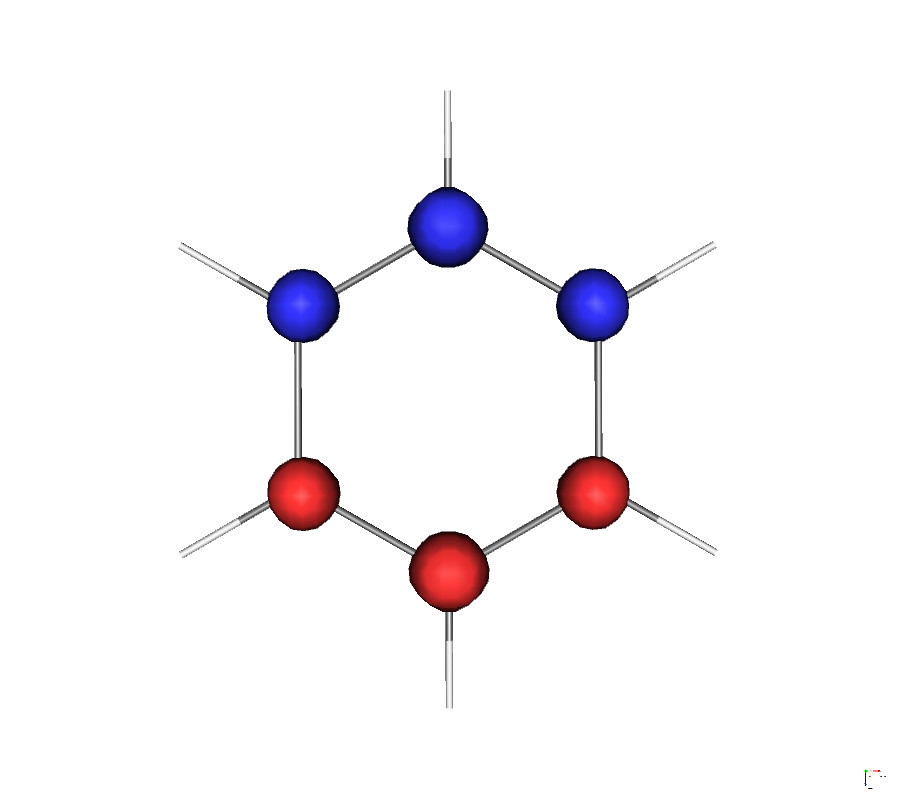
\includegraphics[width=\textwidth]{Benzol-4.png}
		\caption[Network2]{{\small $E_4=-315.2577\,\mathrm{eV}$}}
	\end{subfigure}
	\vskip\baselineskip
	\begin{subfigure}[b]{0.23\textwidth}   
		\centering 
		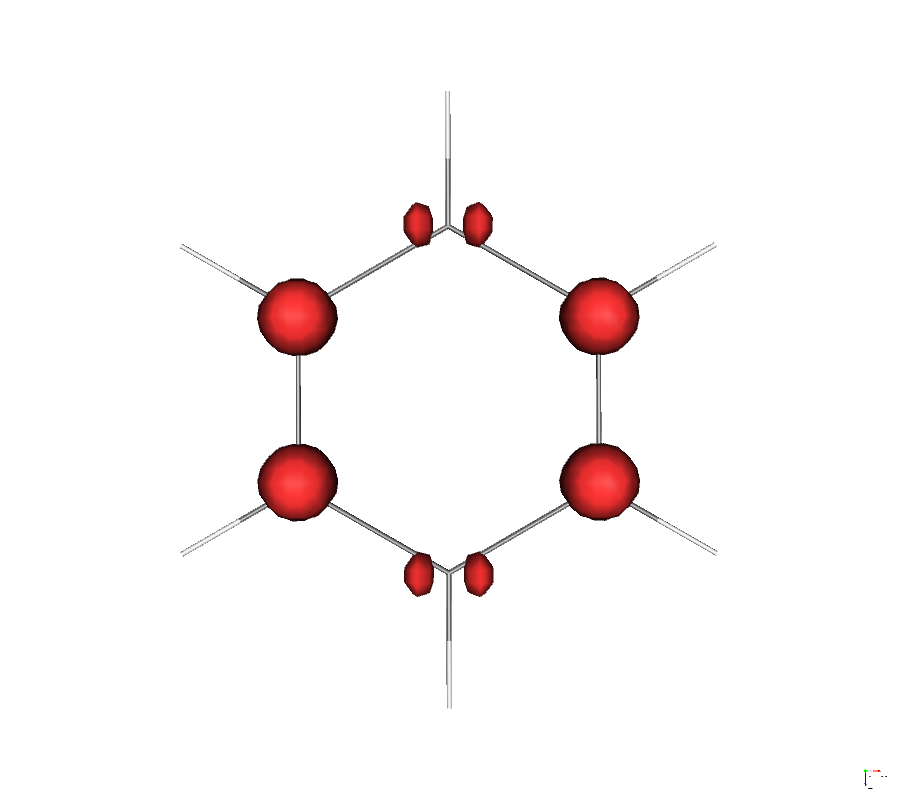
\includegraphics[width=\textwidth]{Benzol-5.png}
		\caption[]{{\small $E_5=-315.2577\,\mathrm{eV}$}}    
	\end{subfigure}
	\hfill
	\begin{subfigure}[b]{0.23\textwidth}   
		\centering 
		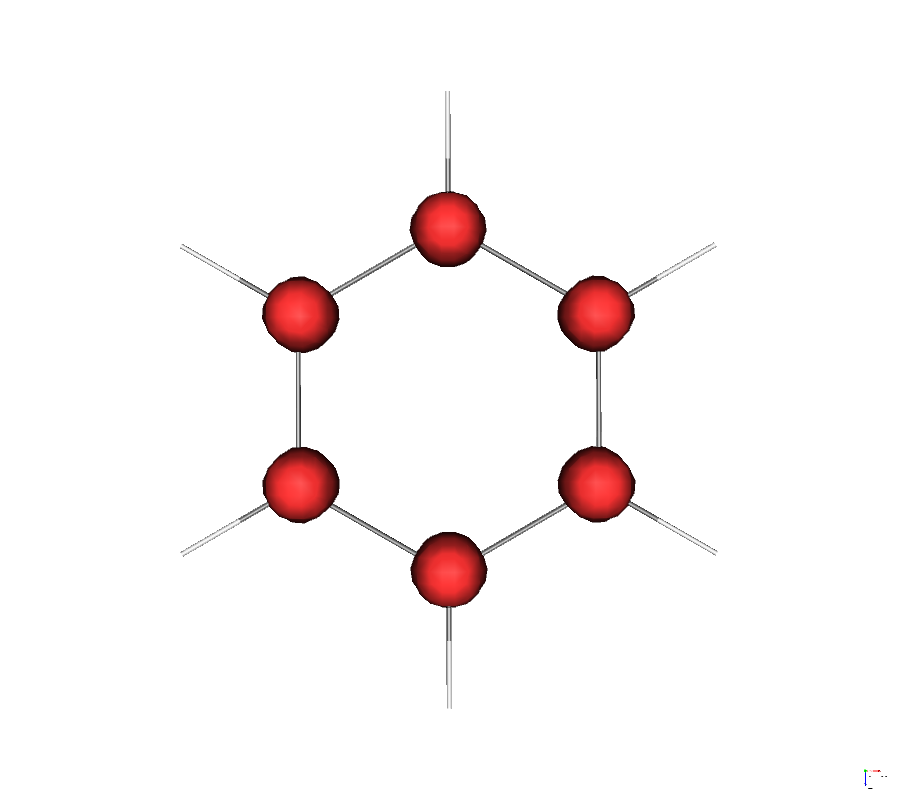
\includegraphics[width=\textwidth]{Benzol-6.png}
		\caption[]{{\small $E_6=-312.4730\,\mathrm{eV}$}}    
	\end{subfigure}
	\begin{subfigure}[b]{0.23\textwidth}   
		\centering 
		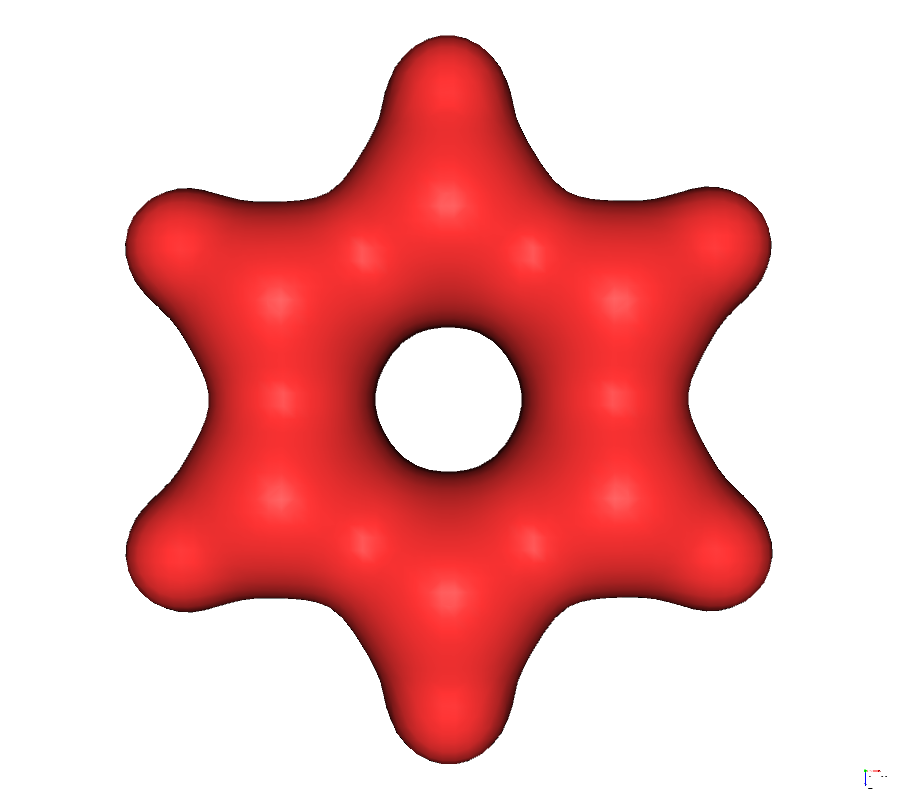
\includegraphics[width=\textwidth]{Benzol-7.png}
		\caption[]{{\small $E_7=-17.6714\,\mathrm{eV}$}}    
	\end{subfigure}
	\hfill
	\begin{subfigure}[b]{0.23\textwidth}   
		\centering 
		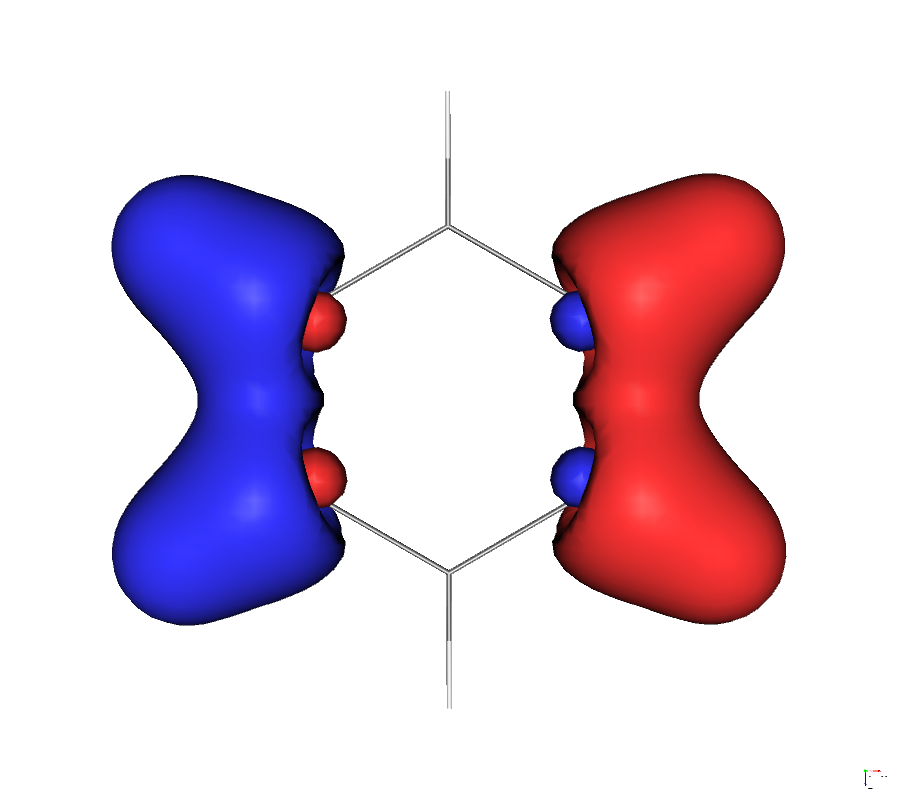
\includegraphics[width=\textwidth]{Benzol-8.png}
		\caption[]{{\small $E_8=-16.8886\,\mathrm{eV}$}}    
	\end{subfigure}
	\vskip\baselineskip
	\begin{subfigure}[b]{0.23\textwidth}   
		\centering 
		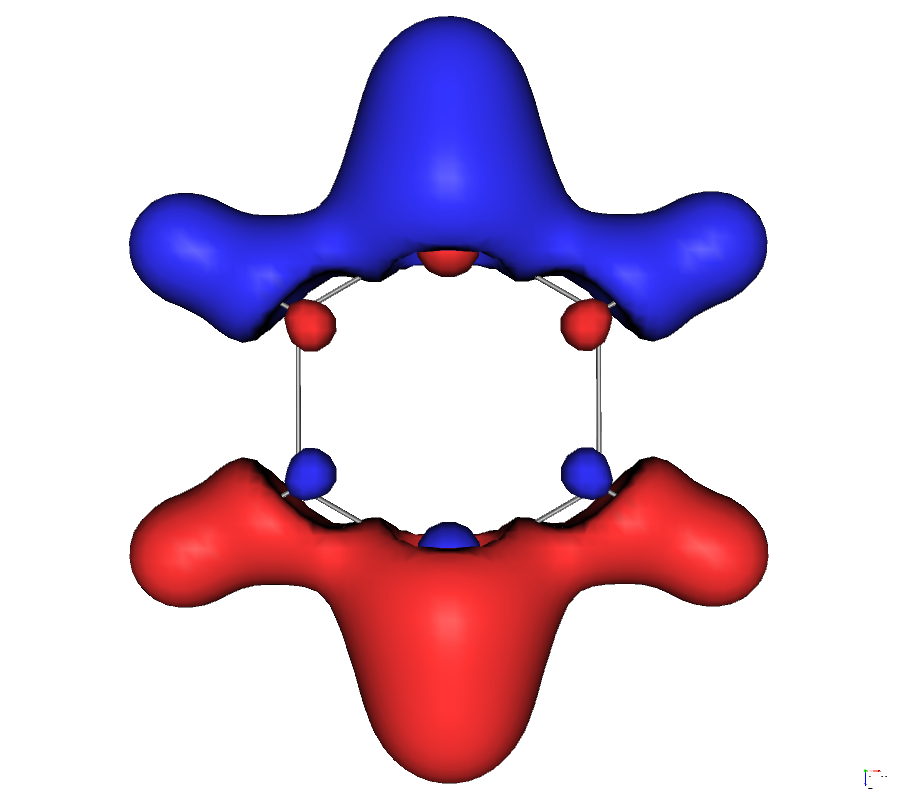
\includegraphics[width=\textwidth]{Benzol-9.png}
		\caption[]{{\small $E_9=-16.8886\,\mathrm{eV}$}}    
	\end{subfigure}
	\hfill
	\begin{subfigure}[b]{0.23\textwidth}   
		\centering 
		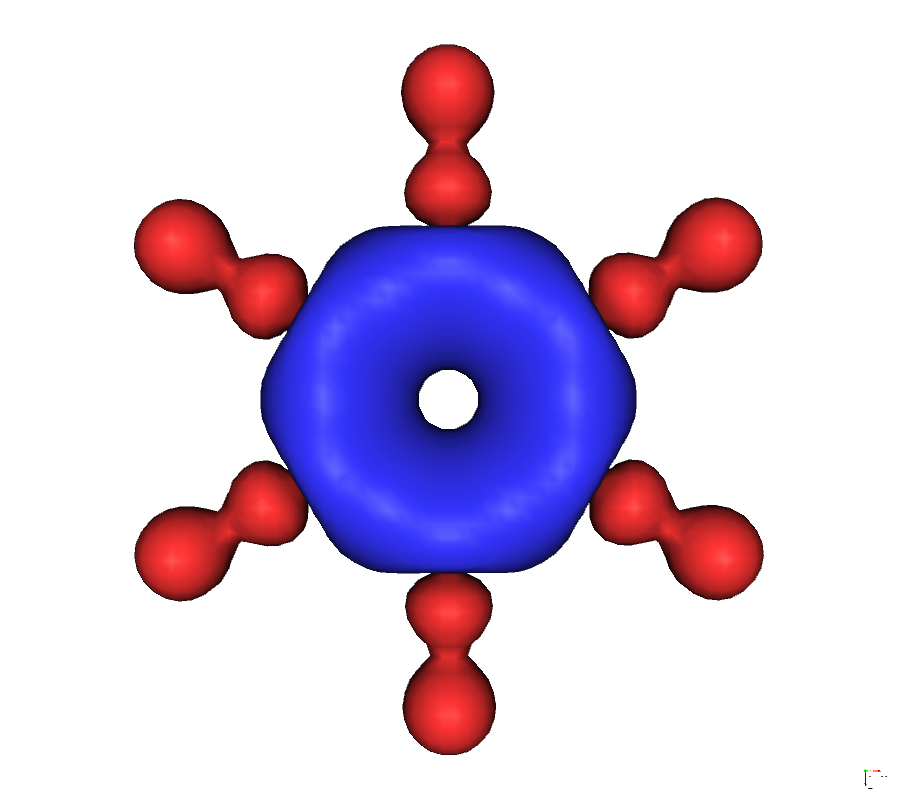
\includegraphics[width=\textwidth]{Benzol-10.png}
		\caption[]{{\small $E_{10}=-15.8940\,\mathrm{eV}$}}    
	\end{subfigure}
	\begin{subfigure}[b]{0.23\textwidth}   
		\centering 
		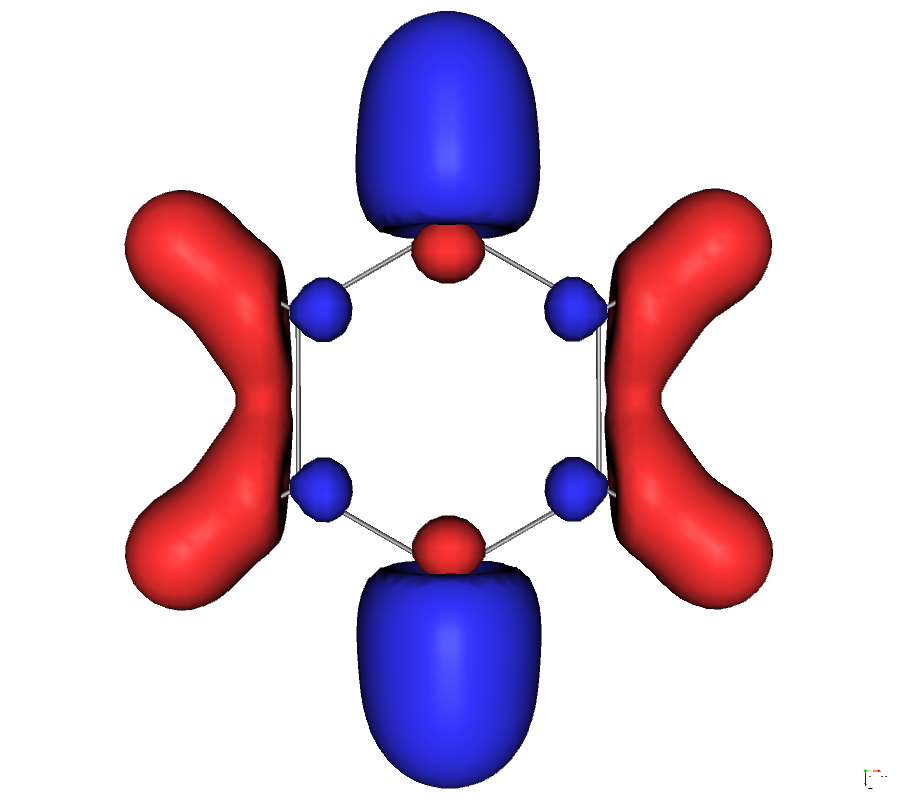
\includegraphics[width=\textwidth]{Benzol-11.png}
		\caption[]{{\small $E_{11}=-15.5864\,\mathrm{eV}$}}    
	\end{subfigure}
	\hfill
	\begin{subfigure}[b]{0.23\textwidth}   
		\centering 
		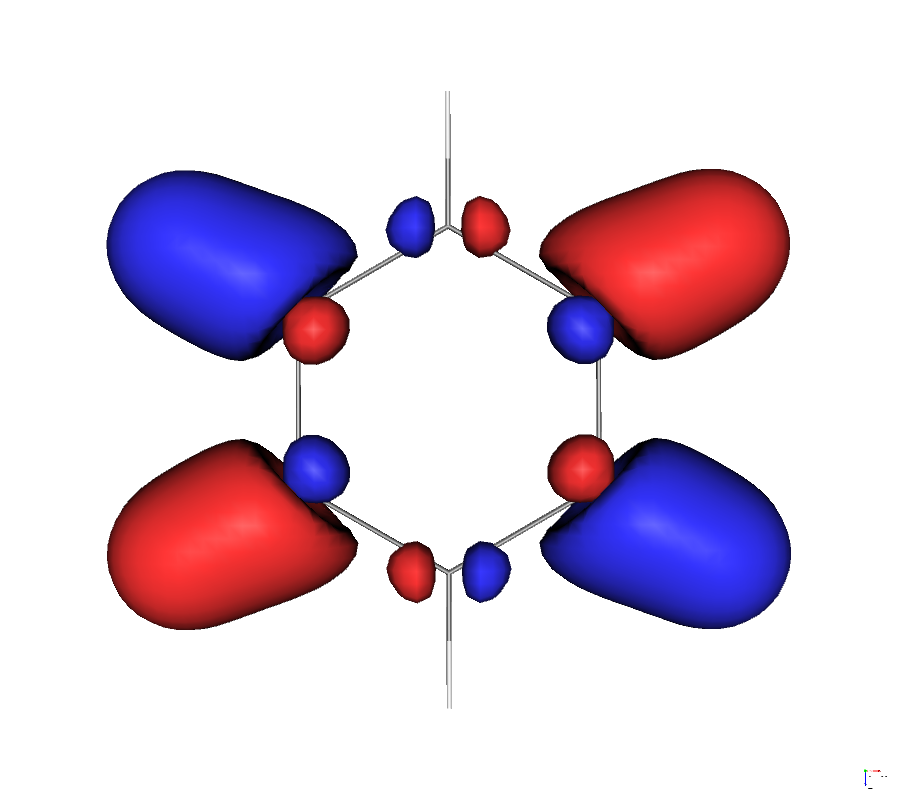
\includegraphics[width=\textwidth]{Benzol-12.png}
		\caption[]{{\small $E_{12}=-15.5864\,\mathrm{eV}$}}    
	\end{subfigure}
	\vskip\baselineskip
	\begin{subfigure}[b]{0.23\textwidth}   
		\centering 
		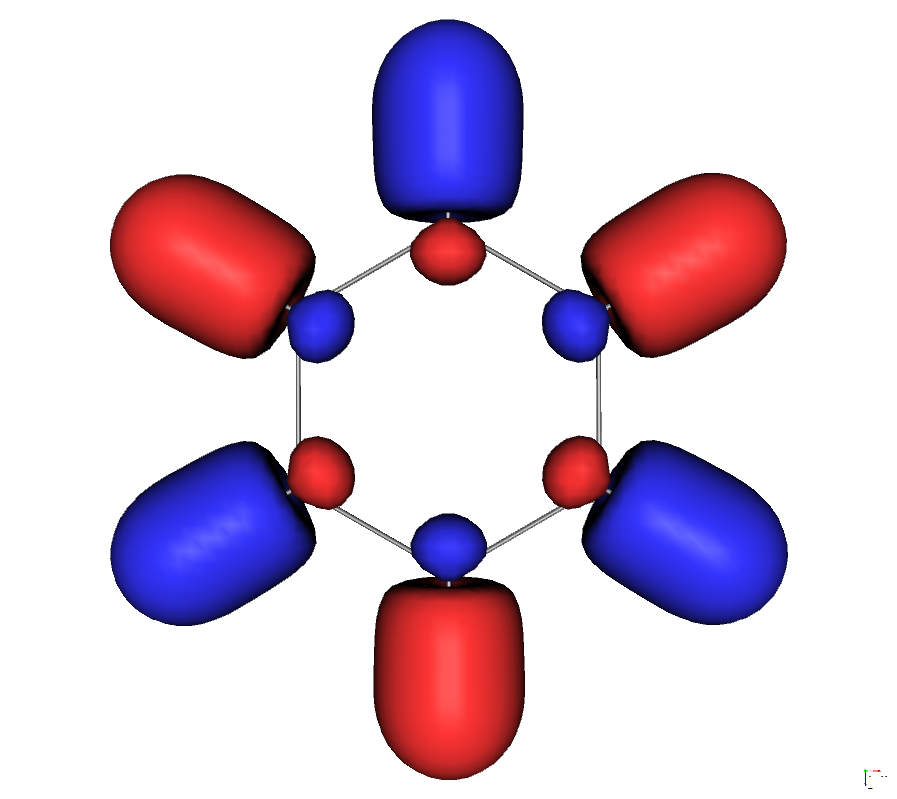
\includegraphics[width=\textwidth]{Benzol-13.png}
		\caption[]{{\small $E_{13}=-14.7920\,\mathrm{eV}$}}    
	\end{subfigure}
	\hfill
	\begin{subfigure}[b]{0.23\textwidth}   
		\centering 
		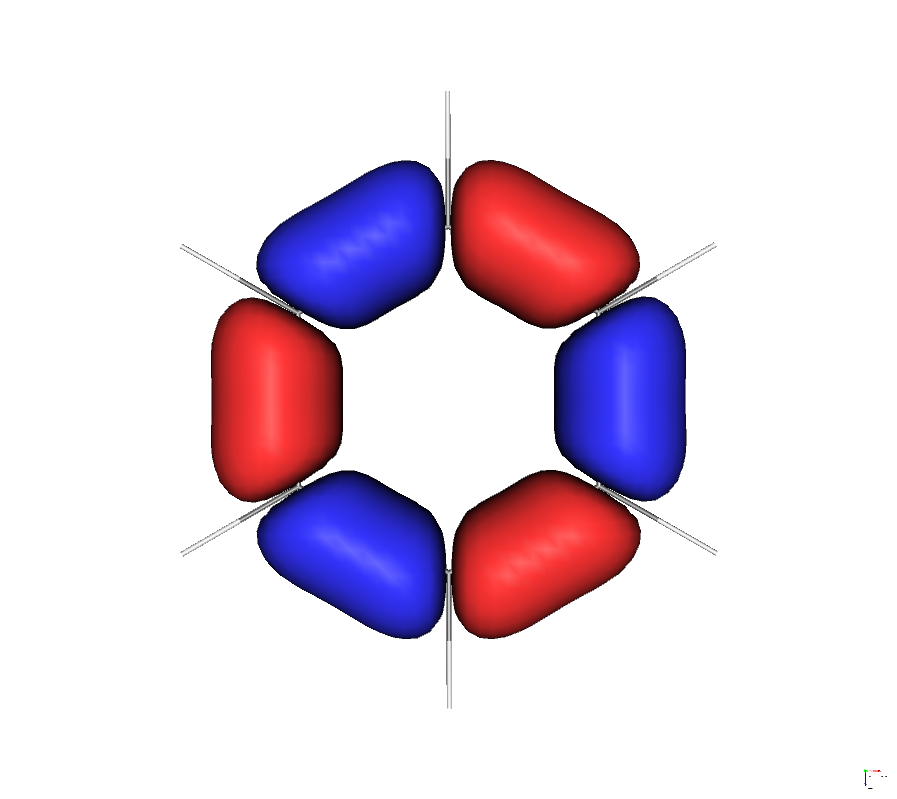
\includegraphics[width=\textwidth]{Benzol-14.png}
		\caption[]{{\small $E_{14}=-14.1467\,\mathrm{eV}$}}    
	\end{subfigure}
	\begin{subfigure}[b]{0.23\textwidth}   
		\centering 
		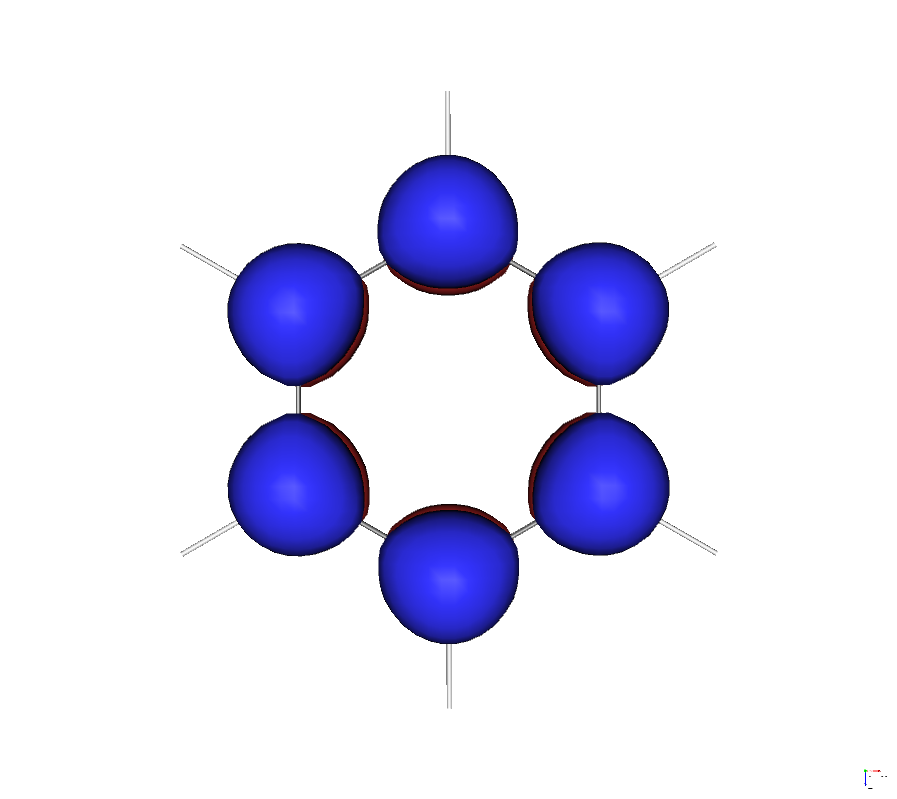
\includegraphics[width=\textwidth]{Benzol-15.png}
		\caption[]{{\small $E_{15}=-13.9999\,\mathrm{eV}$}}    
	\end{subfigure}
	\hfill
	\begin{subfigure}[b]{0.23\textwidth}   
		\centering 
		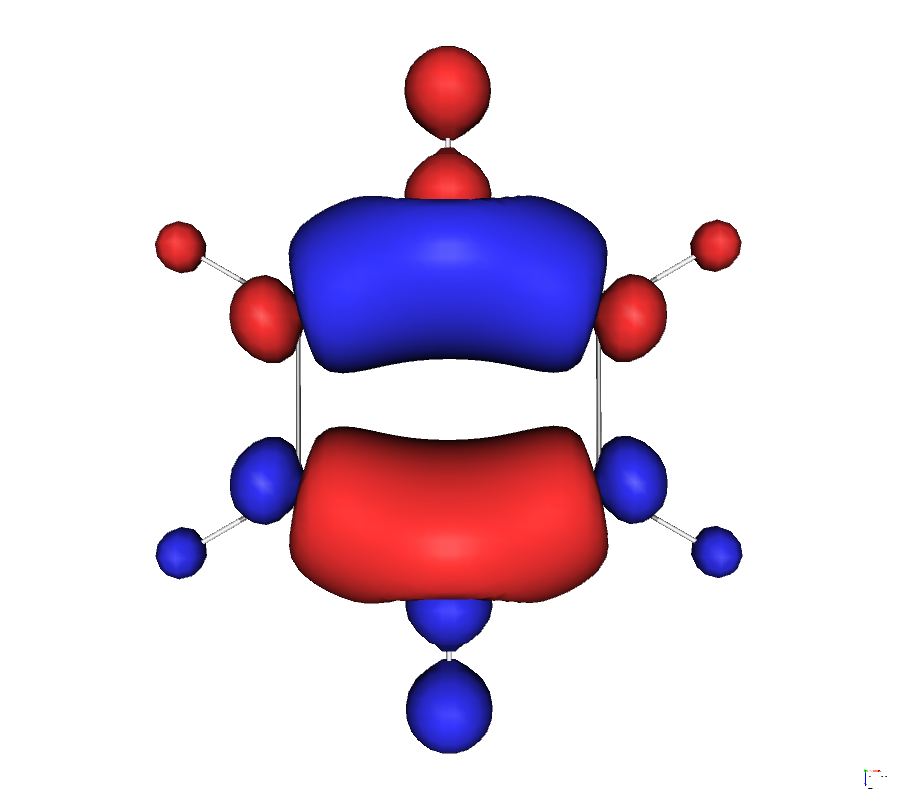
\includegraphics[width=\textwidth]{Benzol-16.png}
		\caption[]{{\small $E_{16}=-13.3536\,\mathrm{eV}$}}    
	\end{subfigure}
	\vskip\baselineskip
	\begin{subfigure}[b]{0.23\textwidth}   
		\centering 
		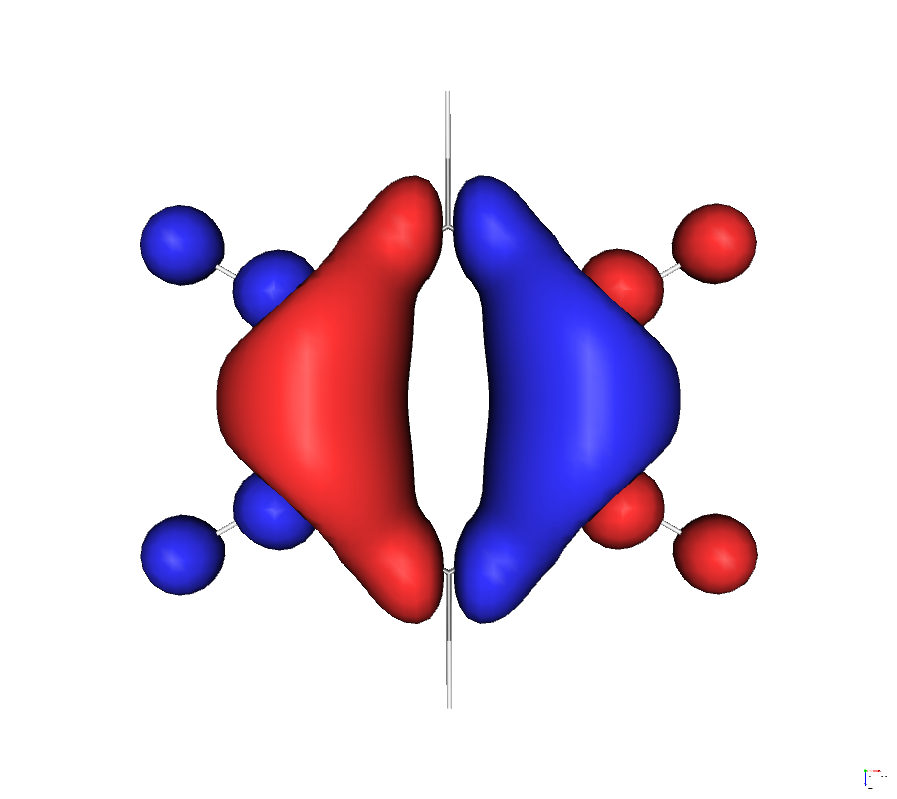
\includegraphics[width=\textwidth]{Benzol-17.png}
		\caption[]{{\small $E_{17}=-13.3536\,\mathrm{eV}$}}    
	\end{subfigure}
	\hfill
	\begin{subfigure}[b]{0.23\textwidth}   
		\centering 
		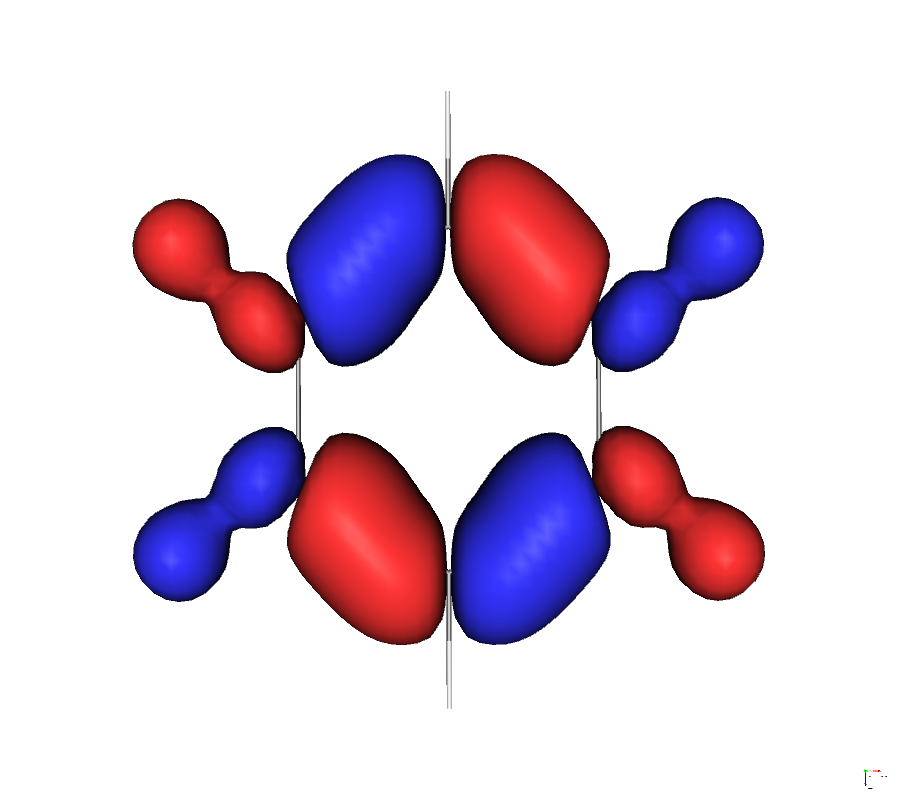
\includegraphics[width=\textwidth]{Benzol-18.png}
		\caption[]{{\small $E_{18}=-12.8376\,\mathrm{eV}$}}    
	\end{subfigure}
	\begin{subfigure}[b]{0.23\textwidth}   
		\centering 
		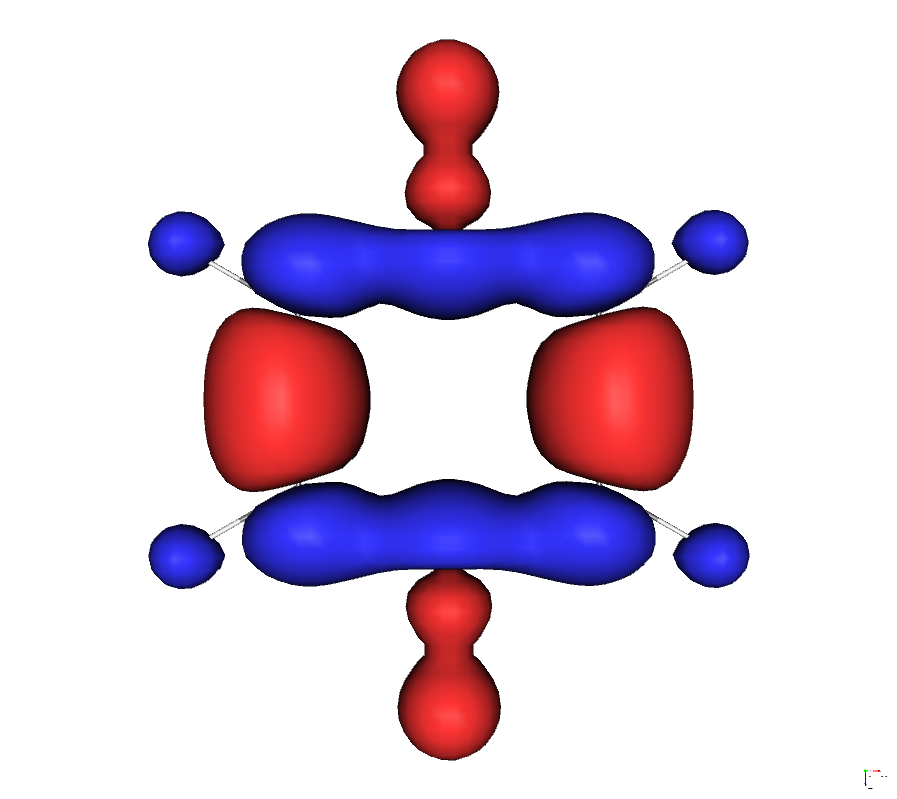
\includegraphics[width=\textwidth]{Benzol-19.png}
		\caption[]{{\small $E_{19}=-12.8376\,\mathrm{eV}$}}    
	\end{subfigure}
	\hfill
	\begin{subfigure}[b]{0.23\textwidth}   
		\centering 
		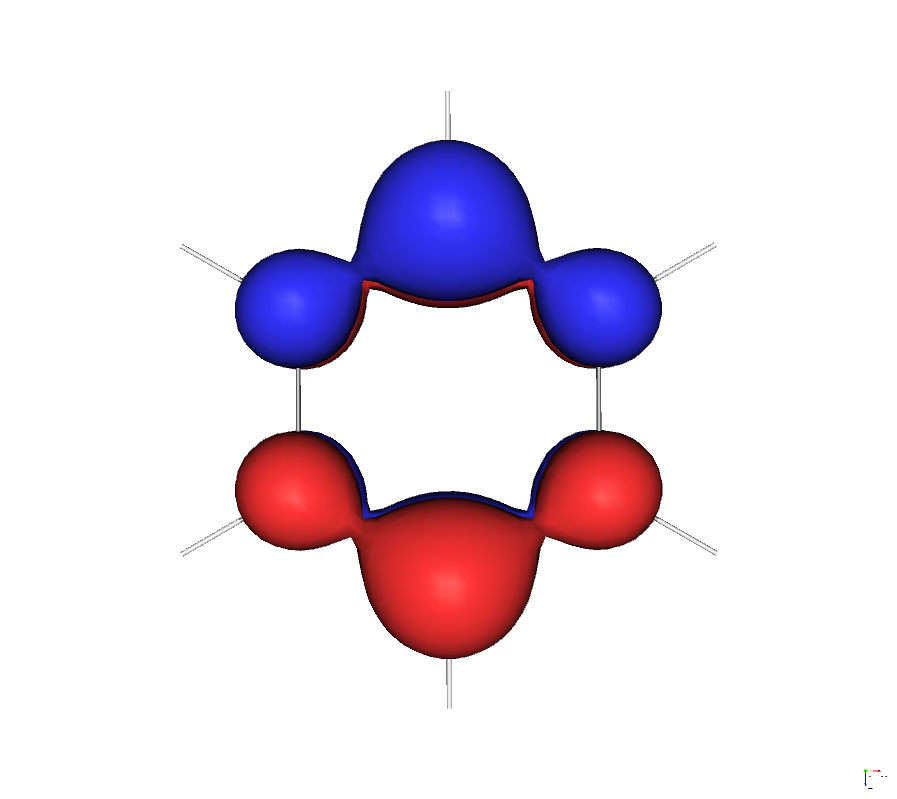
\includegraphics[width=\textwidth]{Benzol-20.png}
		\caption[]{{\small $E_{20}=-12.5459\,\mathrm{eV}$}}    
	\end{subfigure}
\end{figure}





























































\end{document}








